\chapter{\ifproject%
\ifenglish Project Structure and Methodology\else โครงสร้างและขั้นตอนการทำงาน\fi
\else%
\ifenglish Project Structure\else โครงสร้างของโครงงาน\fi
\fi
}

\makeatother

\section{ภาพรวมของระบบ}
ระบบบริหารจัดการห่วงโซ่อุปทานสำหรับการขนส่งสินค้าควบคุมอุณหภูมินี้ ถูกพัฒนาขึ้นโดยมีวัตถุประสงค์เพื่อเพิ่มความโปร่งใสและความน่าเชื่อถือของข้อมูลสภาพแวดล้อมระหว่างการขนส่ง โดยบูรณาการเทคโนโลยีบล็อกเชน (Blockchain) ร่วมกับเทคโนโลยีอินเทอร์เน็ตของสรรพสิ่ง (Internet of Things: IoT) เพื่อให้สามารถตรวจสอบและติดตามข้อมูลอุณหภูมิแบบเรียลไทม์ได้อย่างแม่นยำ โดยระบบมีองค์ประกอบหลักดังนี้:
\begin{itemize}
    \item \textbf{ระบบการนำเข้าและตรวจจับข้อมูล:} ใช้เซนเซอร์ IoT บันทึกอุณหภูมิและแอปพลิเคชันสำหรับเจ้าหน้าที่ป้อนข้อมูล
    \item \textbf{ระบบประมวลผลและส่งผ่านข้อมูล:} ใช้โปรโตคอล MQTT ในการส่งข้อมูลจาก IoT สู่เซิร์ฟเวอร์
    \item \textbf{ระบบจัดเก็บข้อมูลและบล็อกเชน:} ใช้เครือข่าย Hyperledger Fabric เพื่อบันทึกข้อมูลแบบแก้ไขไม่ได้
    \item \textbf{ระบบเว็บแอปพลิเคชัน:} สำหรับติดตามสถานะ แจ้งเตือนความผิดปกติ และแสดงผลการวิเคราะห์
\end{itemize}

\section{การออกแบบสถาปัตยกรรมของระบบ}
โครงสร้างพื้นฐานของระบบถูกออกแบบโดยแบ่งการทำงานออกเป็นส่วนต่างๆ เพื่อให้มั่นใจว่าการทำงานมีความเสถียร รองรับการขยายขนาด และสามารถนำไปติดตั้งใช้งานจริงได้อย่างสะดวกรวดเร็ว โดยมีการใช้เทคโนโลยีคอนเทนเนอร์ (Docker) ในการบริหารจัดการเซอร์วิสต่าง ๆ บน Amazon EC2 Server ดังแสดงในรูปที่ \ref{fig:system_arch}

\begin{figure}[H]
    \begin{center}
    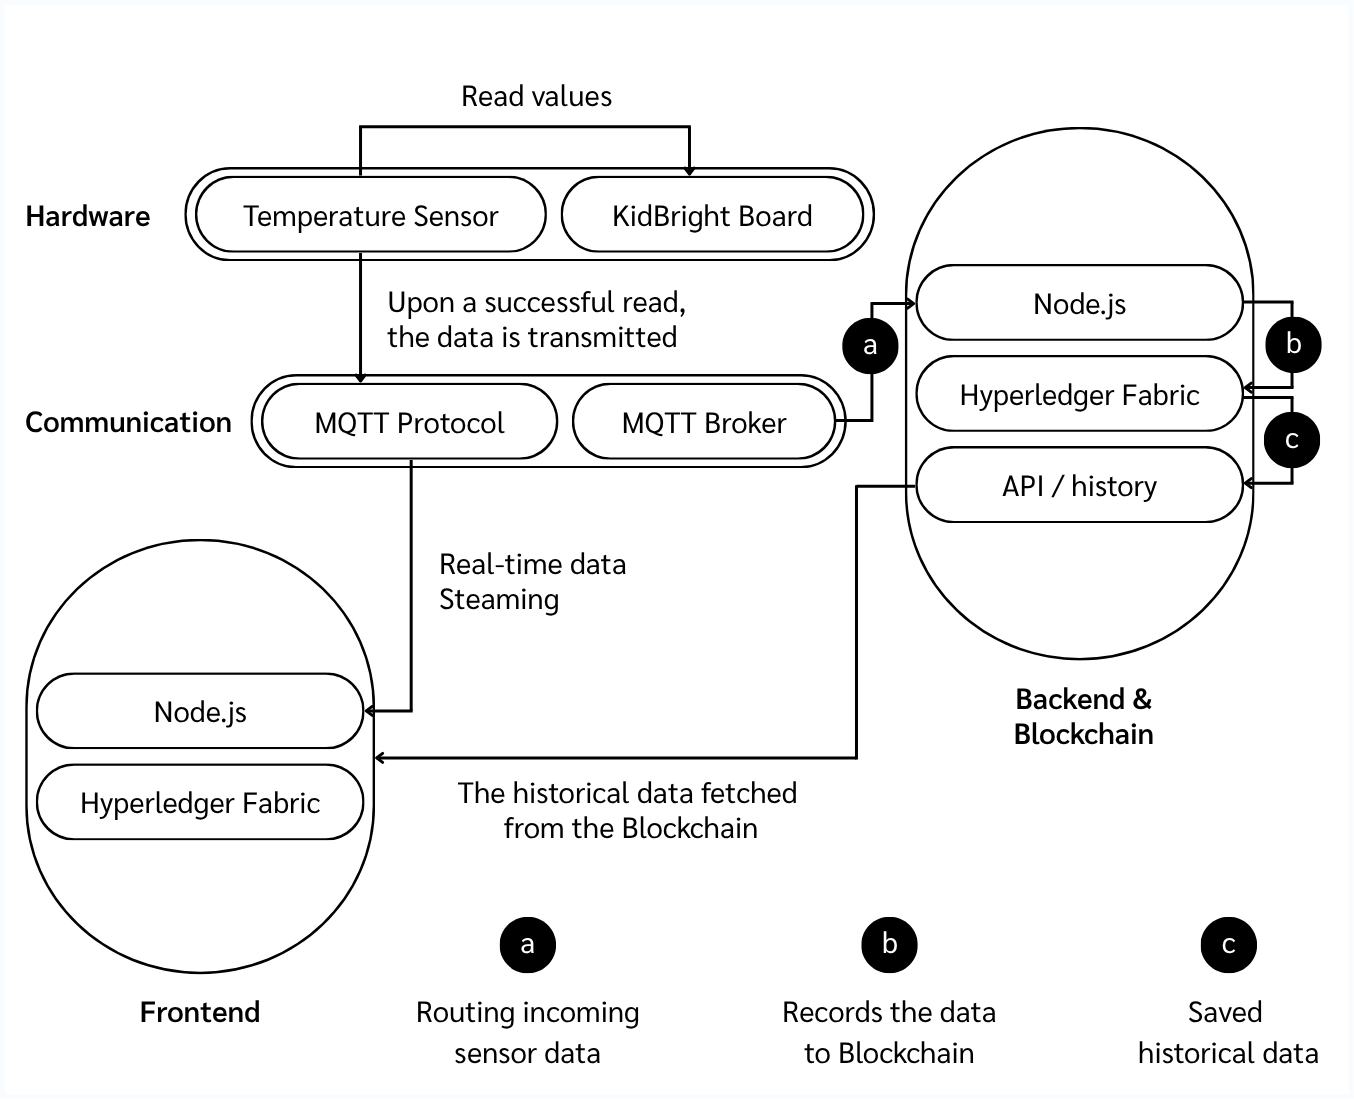
\includegraphics[width=0.9\textwidth]{system arch.png}
    \end{center}
    \caption{การออกแบบสถาปัตยกรรมและการทำงานของระบบ}
    \label{fig:system_arch}
\end{figure}

\section{การออกแบบฮาร์ดแวร์และอุปกรณ์ IoT}
ในส่วนของการตรวจจับข้อมูล อาศัยเซนเซอร์วัดอุณหภูมิที่ติดตั้งไว้ภายในกล่องบรรจุสินค้า เพื่อทำหน้าที่ตรวจวัดและบันทึกค่าอุณหภูมิที่เกิดขึ้นจริงอย่างต่อเนื่องตลอดกระบวนการขนส่ง โดยมีการออกแบบวงจรและลักษณะของอุปกรณ์ดังนี้

\begin{figure}[H]
    \begin{center}
    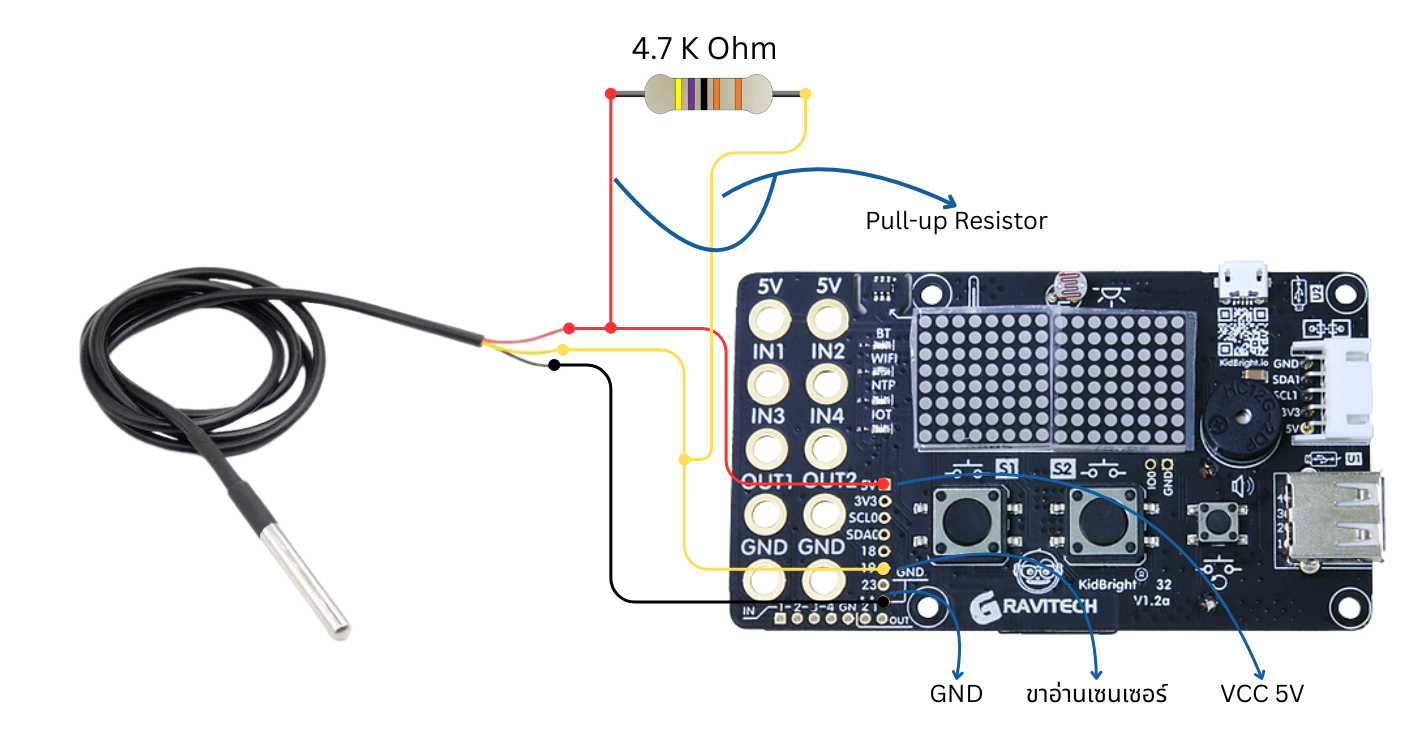
\includegraphics[width=0.8\textwidth]{492 Diagram.png}
    \end{center}
    \caption{แผนผังการต่อวงจรไมโครคอนโทรลเลอร์และเซนเซอร์วัดอุณหภูมิ}
    \label{fig:wiring_diagram}
\end{figure}

\begin{figure}[H]
    \begin{center}
    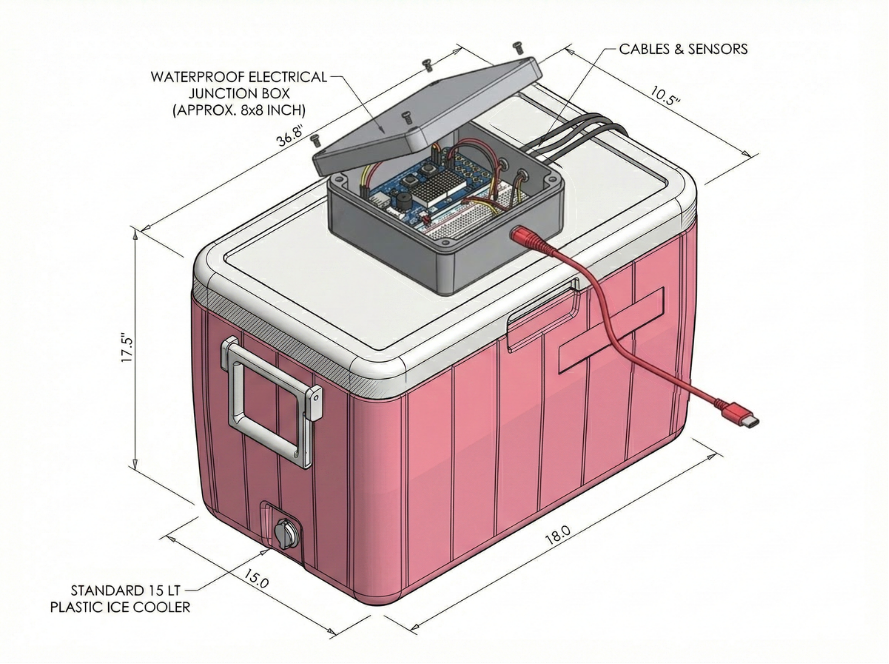
\includegraphics[width=0.8\textwidth]{IoT Box Design.png}
    \end{center}
    \caption{การออกแบบกล่องบรรจุสินค้าและตำแหน่งติดตั้งอุปกรณ์ IoT}
    \label{fig:iot_box}
\end{figure}

\section{ขั้นตอนการดำเนินงานของระบบ}
การทำงานของระบบถูกออกแบบให้ครอบคลุมตั้งแต่ต้นทางจนถึงปลายทางการขนส่ง โดยมีขั้นตอนดังต่อไปนี้:

\subsection{การบันทึกข้อมูลสินค้า}
\begin{itemize}
    \item เจ้าหน้าที่ดำเนินการป้อนข้อมูลที่เกี่ยวข้องกับการขนส่ง เช่น ข้อมูลผู้ส่ง ข้อมูลผู้รับ รายละเอียดของสินค้า และช่วงอุณหภูมิควบคุมที่กำหนด
    \item ระบบจะทำการสร้างรายการขนส่งและออกหมายเลขติดตามพัสดุ เพื่อใช้สำหรับตรวจสอบสถานะของสินค้าตลอดกระบวนการ
\end{itemize}

\subsection{การตรวจสอบและบันทึกอุณหภูมิแบบเรียลไทม์}
\begin{itemize}
    \item อุปกรณ์เซนเซอร์ IoT ที่ติดตั้งบริเวณกล่องบรรจุสินค้า จะทำการวัดค่าอุณหภูมิอย่างต่อเนื่อง และส่งข้อมูลผ่านเครือข่ายอินเทอร์เน็ตไปยัง Amazon EC2 Server
    \item ข้อมูลอุณหภูมิจะถูกส่งผ่านโปรโตคอล MQTT เพื่อนำไปแสดงผล และถูกส่งไปบันทึกลงในระบบบล็อกเชน (Hyperledger Fabric) ผ่าน Smart Contract เพื่อรับประกันความปลอดภัยและป้องกันการแก้ไขข้อมูลย้อนหลัง
    \item ผู้มีส่วนได้ส่วนเสียสามารถติดตามสถานะอุณหภูมิของสินค้าได้แบบเรียลไทม์ผ่านเว็บแอปพลิเคชัน
\end{itemize}

\subsection{การแจ้งเตือนเมื่อพบค่าผิดปกติ}
\begin{itemize}
    \item หากอุณหภูมิของสินค้าสูงหรือต่ำกว่าช่วงที่กำหนด ระบบจะแสดงการแจ้งเตือนบนแพลตฟอร์มเว็บไซต์ทันที
    \item เจ้าหน้าที่หรือผู้ควบคุมระบบสามารถรับทราบปัญหา และดำเนินการแก้ไขสถานการณ์ หรือแจ้งให้ผู้ที่เกี่ยวข้องทราบได้อย่างทันท่วงที เพื่อลดความเสียหายของสินค้า
\end{itemize}

\subsection{การติดตามสถานะและการแสดงผล}
\begin{itemize}
    \item ในระหว่างกระบวนการขนส่ง ระบบจะแสดงผลเฉพาะค่าอุณหภูมิและสถานะปัจจุบันแบบเรียลไทม์บนเว็บแอปพลิเคชัน เพื่อมุ่งเน้นให้ผู้ใช้งานสามารถเฝ้าระวังอุณหภูมิและรับมือกับความผิดปกติได้อย่างทันท่วงที
    \item เมื่อกระบวนการขนส่งเสร็จสมบูรณ์ ระบบจะทำการดึงข้อมูลอุณหภูมิที่ถูกบันทึกไว้ตลอดการเดินทางมาประมวลผล เพื่อแสดงผลในรูปแบบกราฟเชิงเวลา (Time-series Graph) โดยกราฟจะแสดงให้เห็นถึงการเปลี่ยนแปลงของอุณหภูมิตั้งแต่จุดเริ่มต้นการจัดส่งจนถึงจุดหมายปลายทาง พร้อมทั้งสรุปค่าทางสถิติเพื่อให้ผู้ใช้งานสามารถวิเคราะห์ภาพรวมของการขนส่งในรอบนั้น ๆ ได้
\end{itemize}

\subsection{การปิดกระบวนการขนส่งและการตรวจสอบย้อนหลัง}
\begin{itemize}
    \item เมื่อสินค้าถูกจัดส่งถึงปลายทางและผู้รับได้ทำการเซ็นยืนยันการรับสินค้าผ่านระบบเรียบร้อยแล้ว กระบวนการขนส่งจะถือว่าสิ้นสุดอย่างสมบูรณ์ และระบบจะบันทึกสถานะการส่งมอบเป็นขั้นตอนสุดท้าย
    \item หลังจากที่สถานะการขนส่งสิ้นสุดลง ระบบจึงจะเปิดสิทธิ์ให้ผู้ใช้งานสามารถเข้าถึงและตรวจสอบประวัติข้อมูลอุณหภูมิย้อนหลัง ได้ตลอดช่วงระยะเวลาการเดินทางของสินค้า
    \item ในขั้นตอนการตรวจสอบ ระบบจะทำการดึงข้อมูลอุณหภูมิทั้งหมดตั้งแต่เริ่มต้นจนถึงจุดหมายปลายทาง มาเปรียบเทียบกับข้อมูลที่ถูกบันทึกไว้ในระบบบล็อกเชน โดยอ้างอิงจากรอยเวลา (Timestamp) ของแต่ละชุดข้อมูล
    \item กระบวนการนี้เป็นหลักฐานพิสูจน์เชิงประจักษ์ว่า ข้อมูลอุณหภูมิระหว่างการขนส่งไม่เคยถูกดัดแปลงหรือแก้ไข ทำให้สามารถใช้อ้างอิงได้ในกรณีที่เกิดปัญหาหรือข้อพิพาทเกี่ยวกับคุณภาพสินค้า
\end{itemize}

\section{การออกแบบส่วนติดต่อผู้ใช้งาน}
การออกแบบหน้าจอของเว็บแอปพลิเคชันถูกพัฒนาขึ้นเพื่อให้ผู้ใช้งานสามารถโต้ตอบกับระบบได้อย่างสะดวกและมีประสิทธิภาพ โดยแบ่งหมวดหมู่การเข้าถึงออกเป็น 4 ส่วนหลัก ได้แก่ หน้าหลัก (Main) ส่วนการยืนยันตัวตน (Auth) ส่วนของผู้ใช้งานทั่วไป (User) และส่วนของผู้ดูแลระบบ (Admin) โดยมีรายละเอียดหน้าจอดังต่อไปนี้

\subsection{หน้าหลัก}
ในส่วนนี้เป็นหน้าต่างแรกสำหรับผู้ใช้งานทุกคนที่เข้ามาสู่แพลตฟอร์ม ประกอบด้วย:

\vspace{1em}
\begin{minipage}{\linewidth}
\noindent \textbf{1. หน้าแรก} \\
หน้าหลักของเว็บไซต์ที่แสดงข้อมูลเบื้องต้นและภาพรวมของบริการ
\begin{figure}[H]
    \centering
    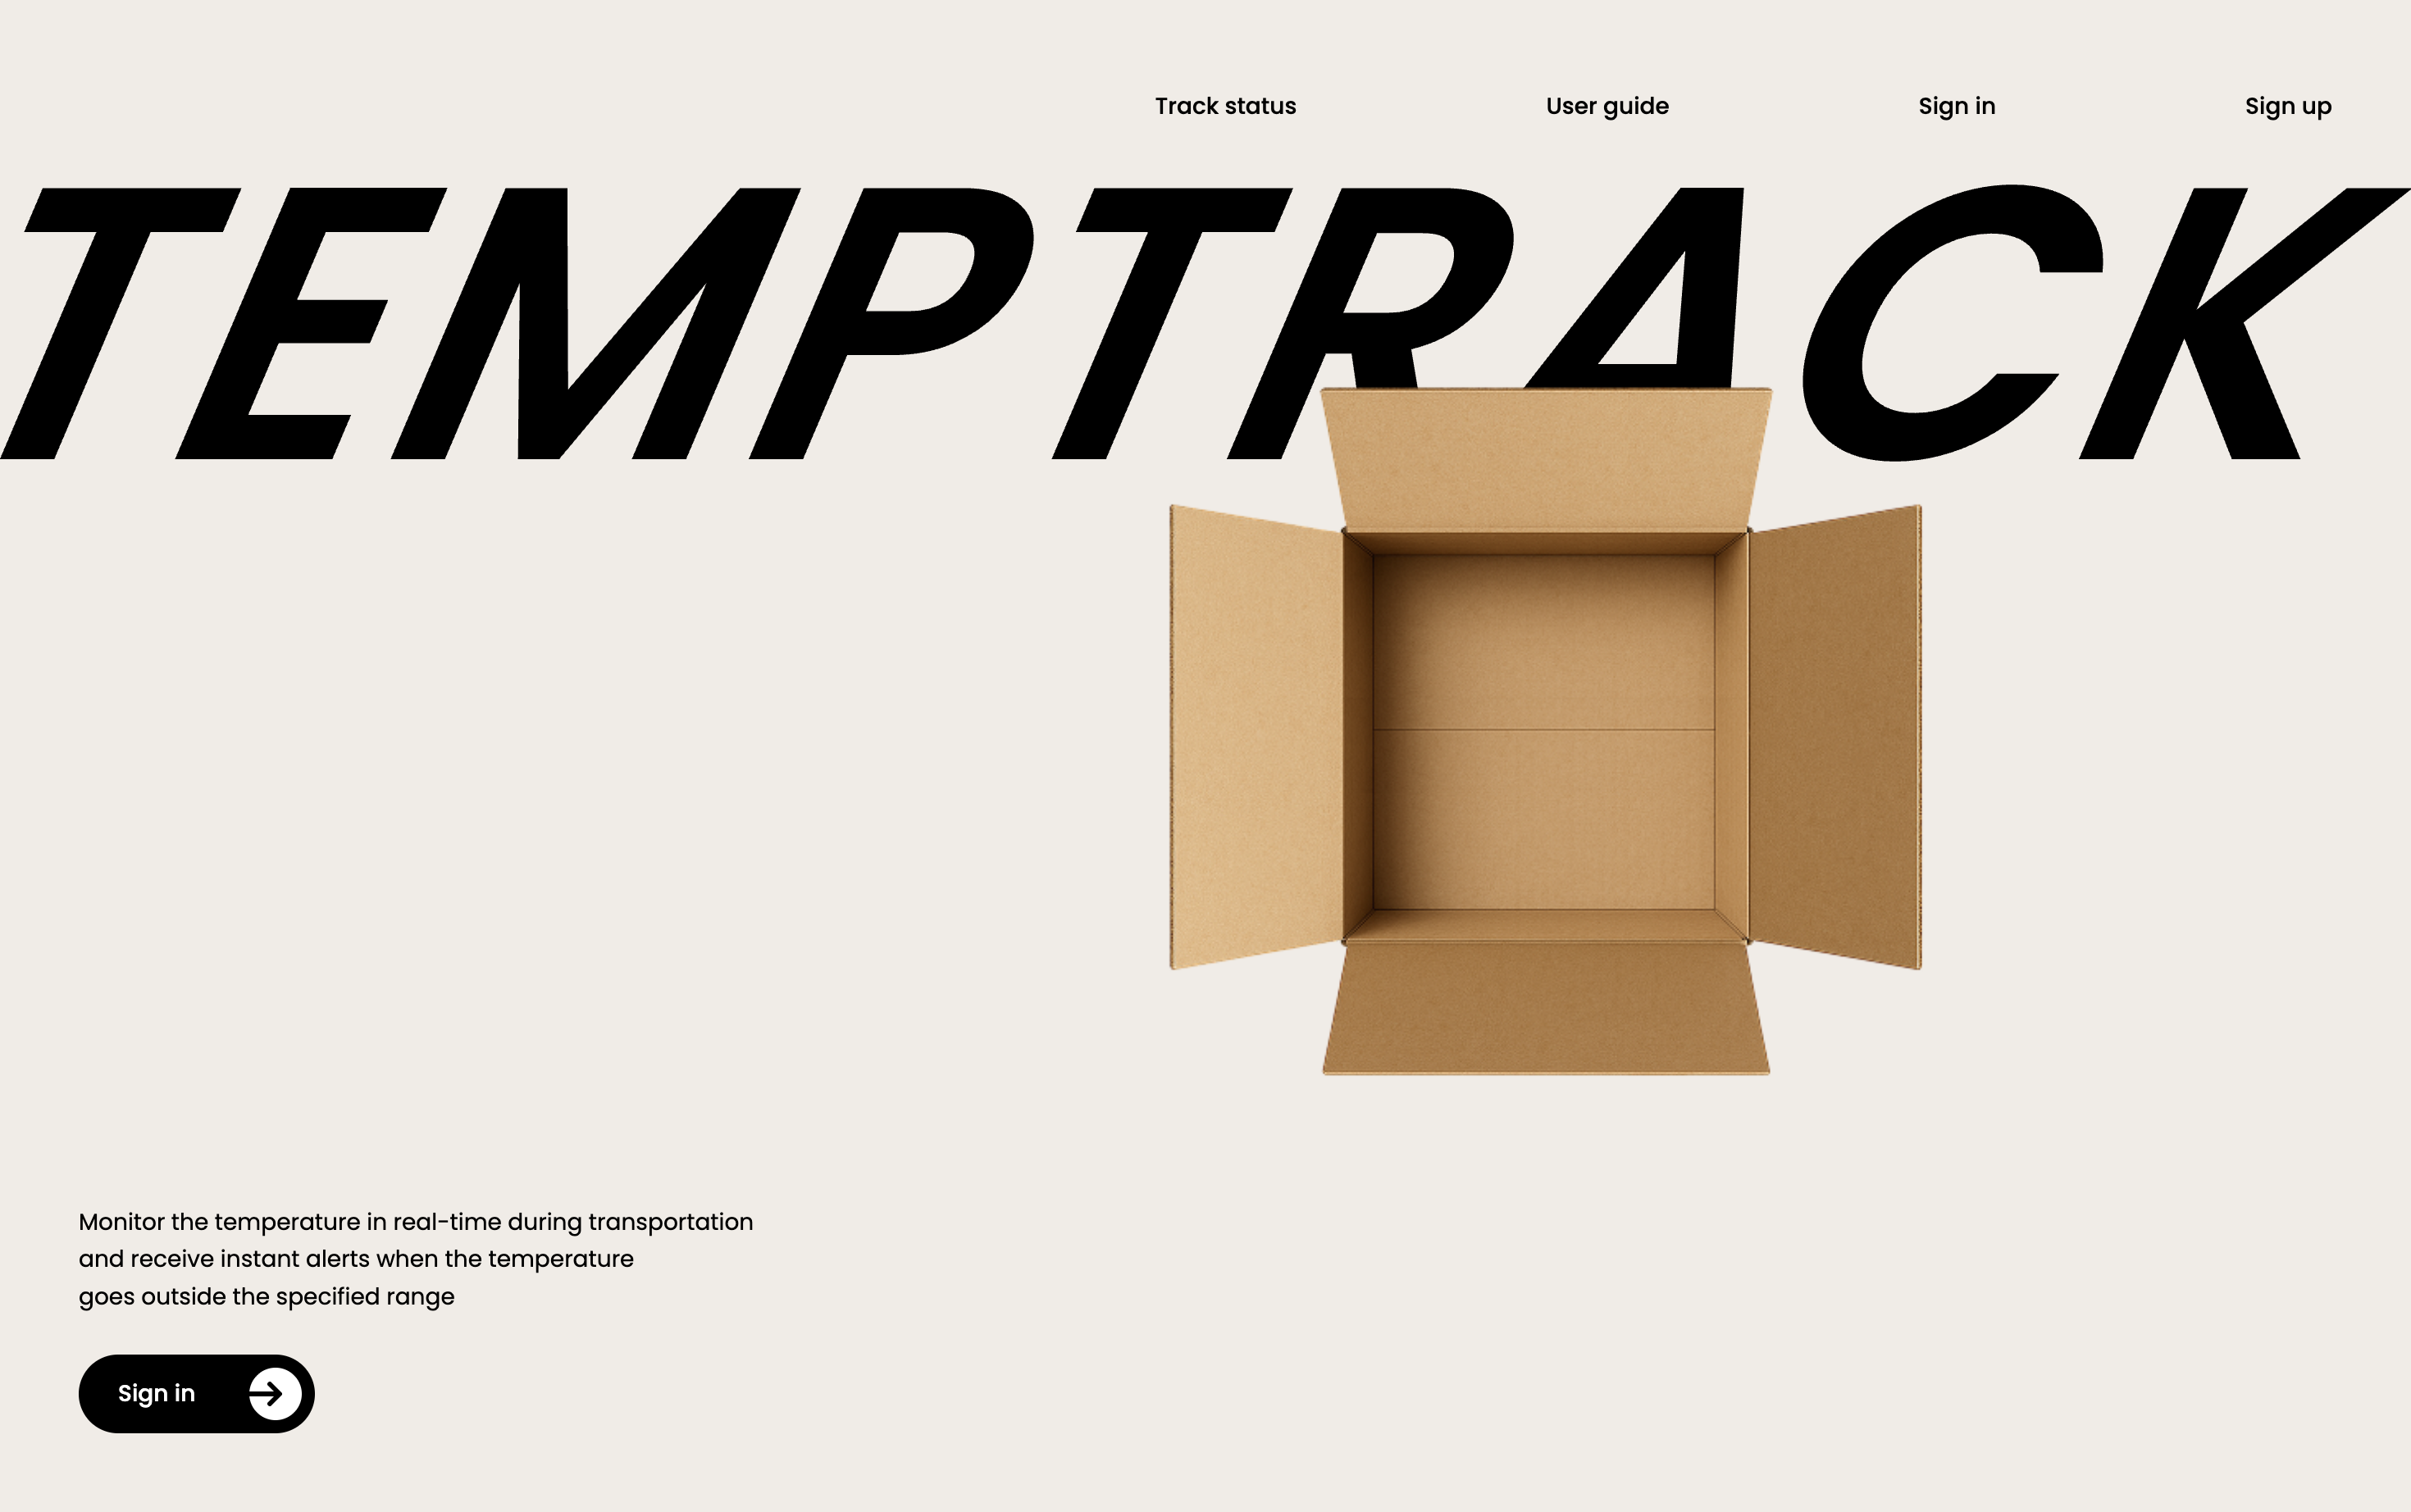
\includegraphics[width=0.8\textwidth]{home.png}
    \caption{หน้าแรก}
    \label{fig:ui_home}
\end{figure}
\end{minipage}

\vspace{1em}
\begin{minipage}{\linewidth}
\noindent \textbf{2. หน้าคู่มือการใช้งาน} \\
อธิบายวิธีการใช้งานแพลตฟอร์มและฟีเจอร์ต่าง ๆ เพื่ออำนวยความสะดวกแก่ผู้ใช้ใหม่
\begin{figure}[H]
    \centering
    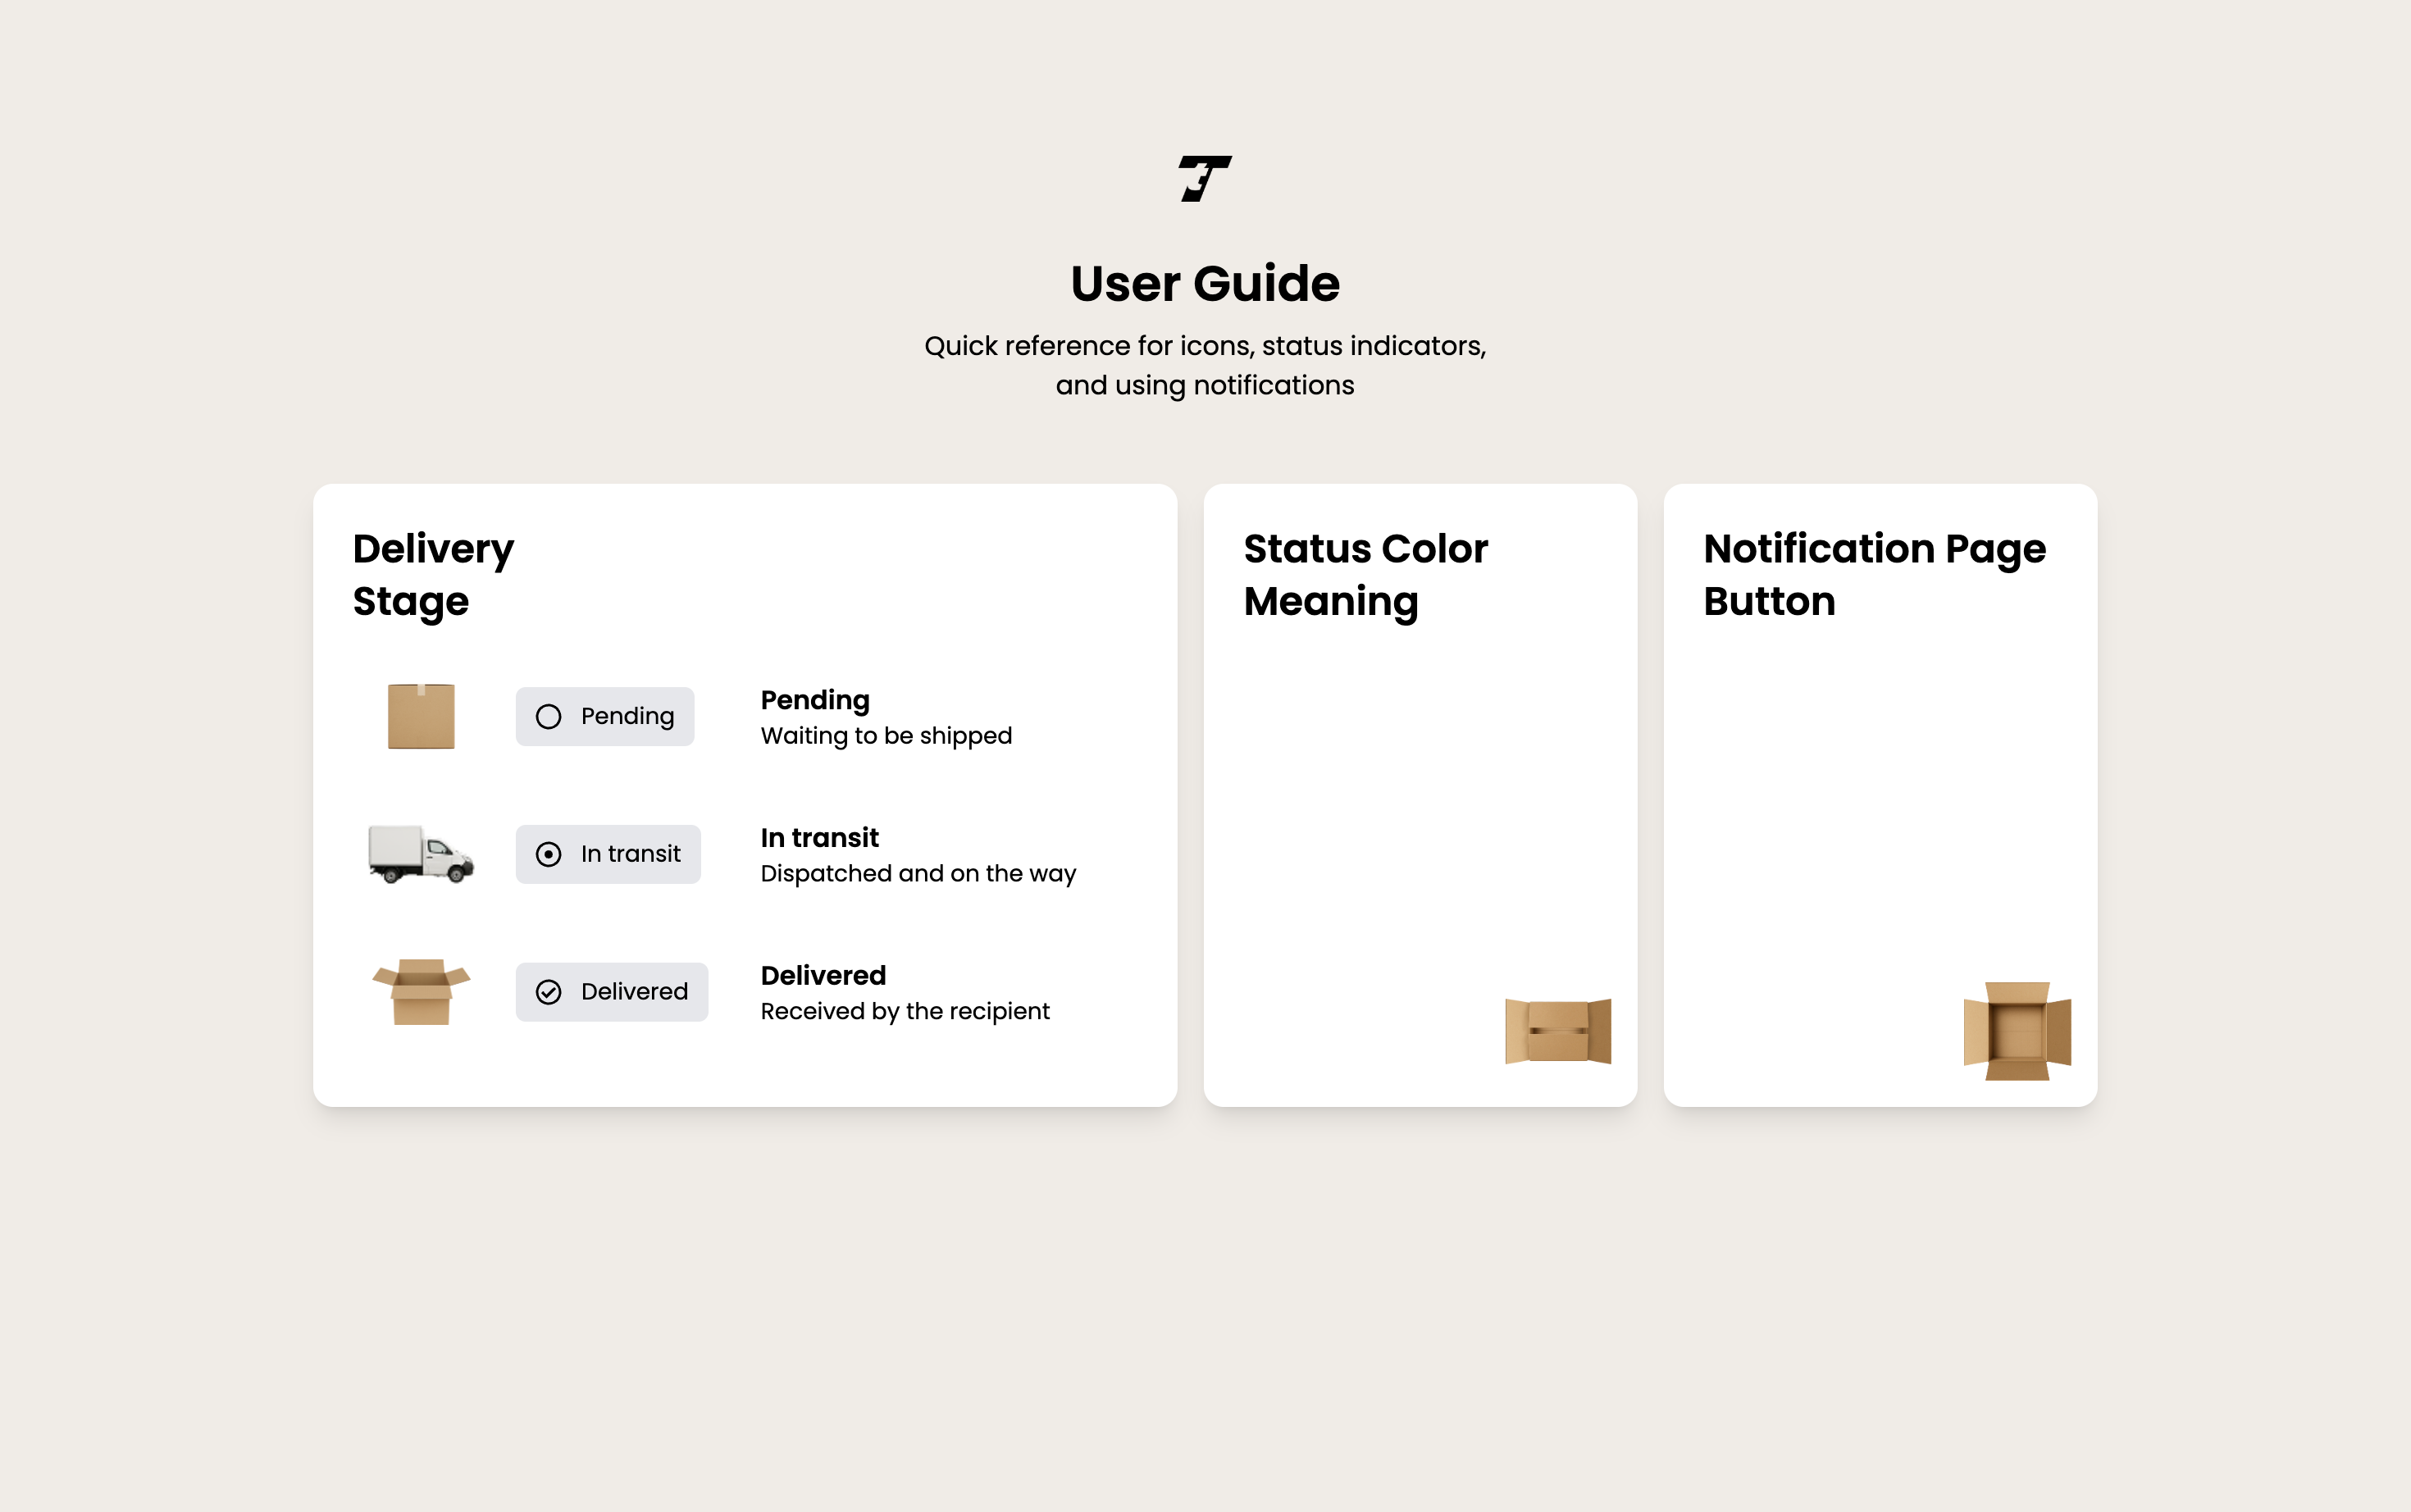
\includegraphics[width=0.8\textwidth]{userguide.png}
    \caption{หน้าคู่มือการใช้งาน}
    \label{fig:ui_guide}
\end{figure}
\end{minipage}


\subsection{ส่วนการยืนยันตัวตน}
ระบบรักษาความปลอดภัยและการเข้าถึงบัญชีผู้ใช้ ประกอบด้วย:

\vspace{1em}
\begin{minipage}{\linewidth}
\noindent \textbf{1. หน้าเข้าสู่ระบบ} \\
สำหรับให้ผู้ใช้งานทั่วไปและผู้ดูแลระบบทำการยืนยันตัวตนเพื่อเข้าสู่ระบบ
\begin{figure}[H]
    \centering
    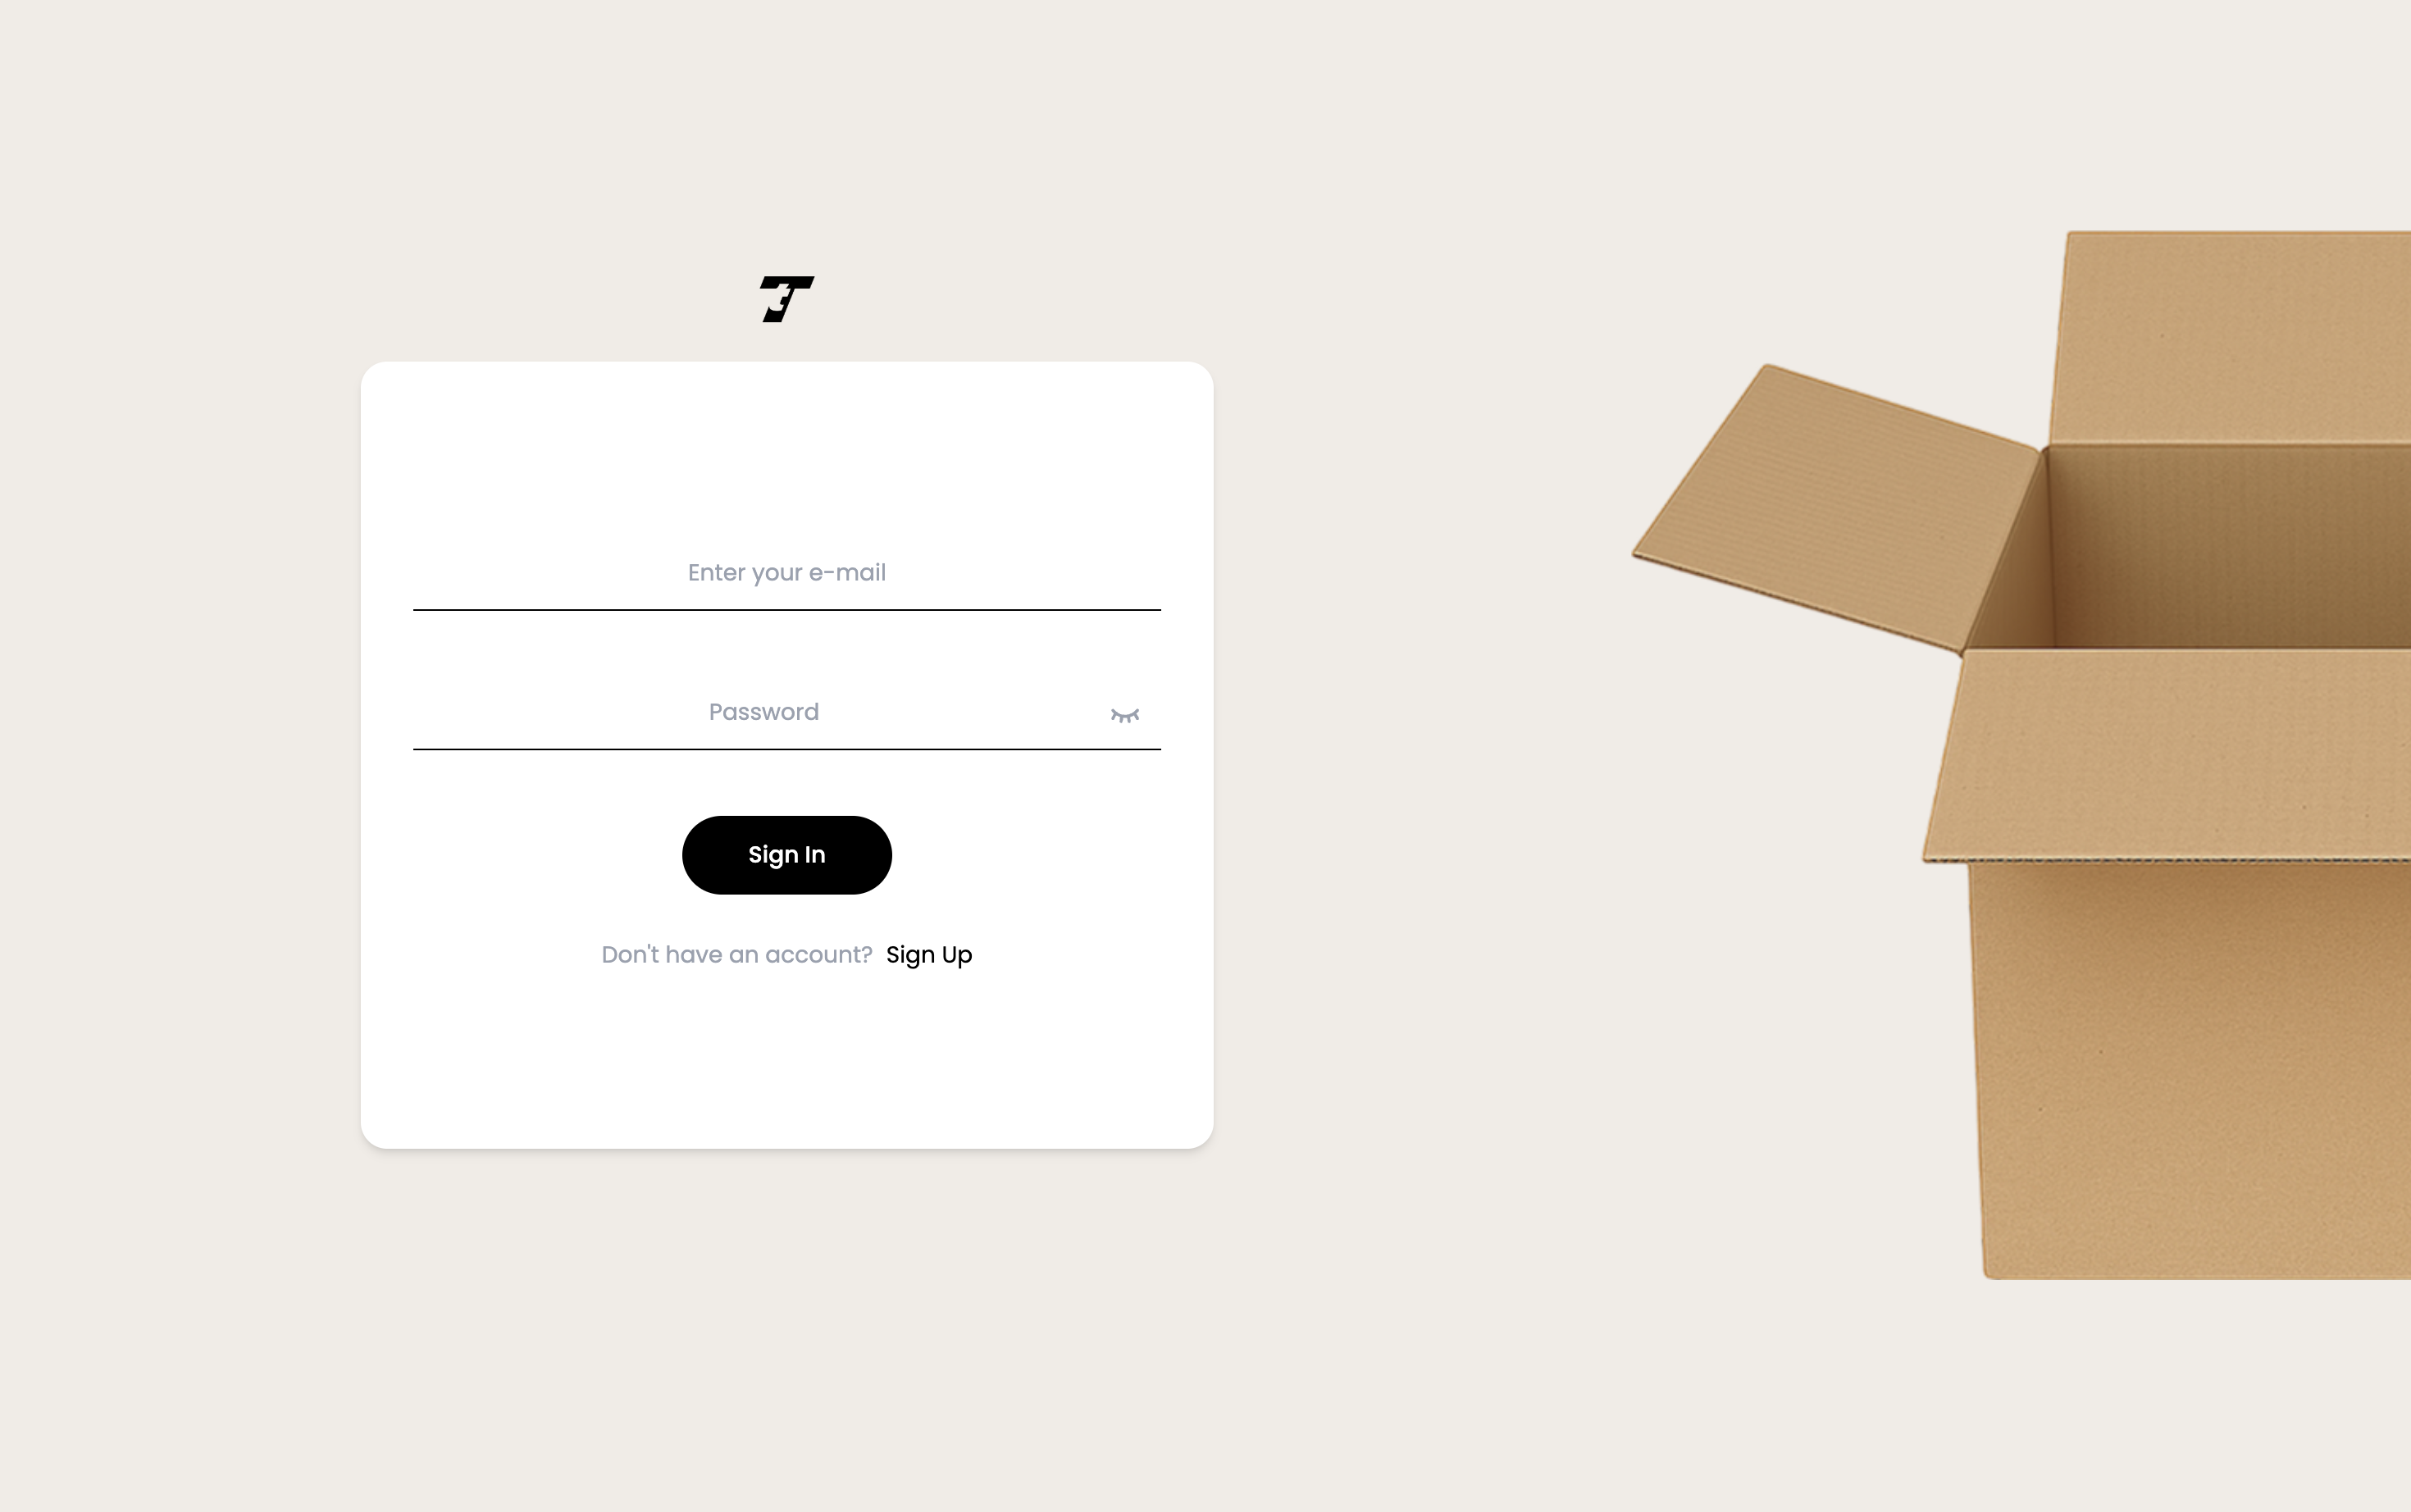
\includegraphics[width=0.8\textwidth]{signin.png}
    \caption{หน้าเข้าสู่ระบบ}
    \label{fig:ui_signin}
\end{figure}
\end{minipage}

\vspace{1em}
\begin{minipage}{\linewidth}
\noindent \textbf{2. หน้าสมัครสมาชิก} \\
สำหรับให้ผู้ใช้งานใหม่ทำการลงทะเบียนและสร้างบัญชีผู้ใช้
\begin{figure}[H]
    \centering
    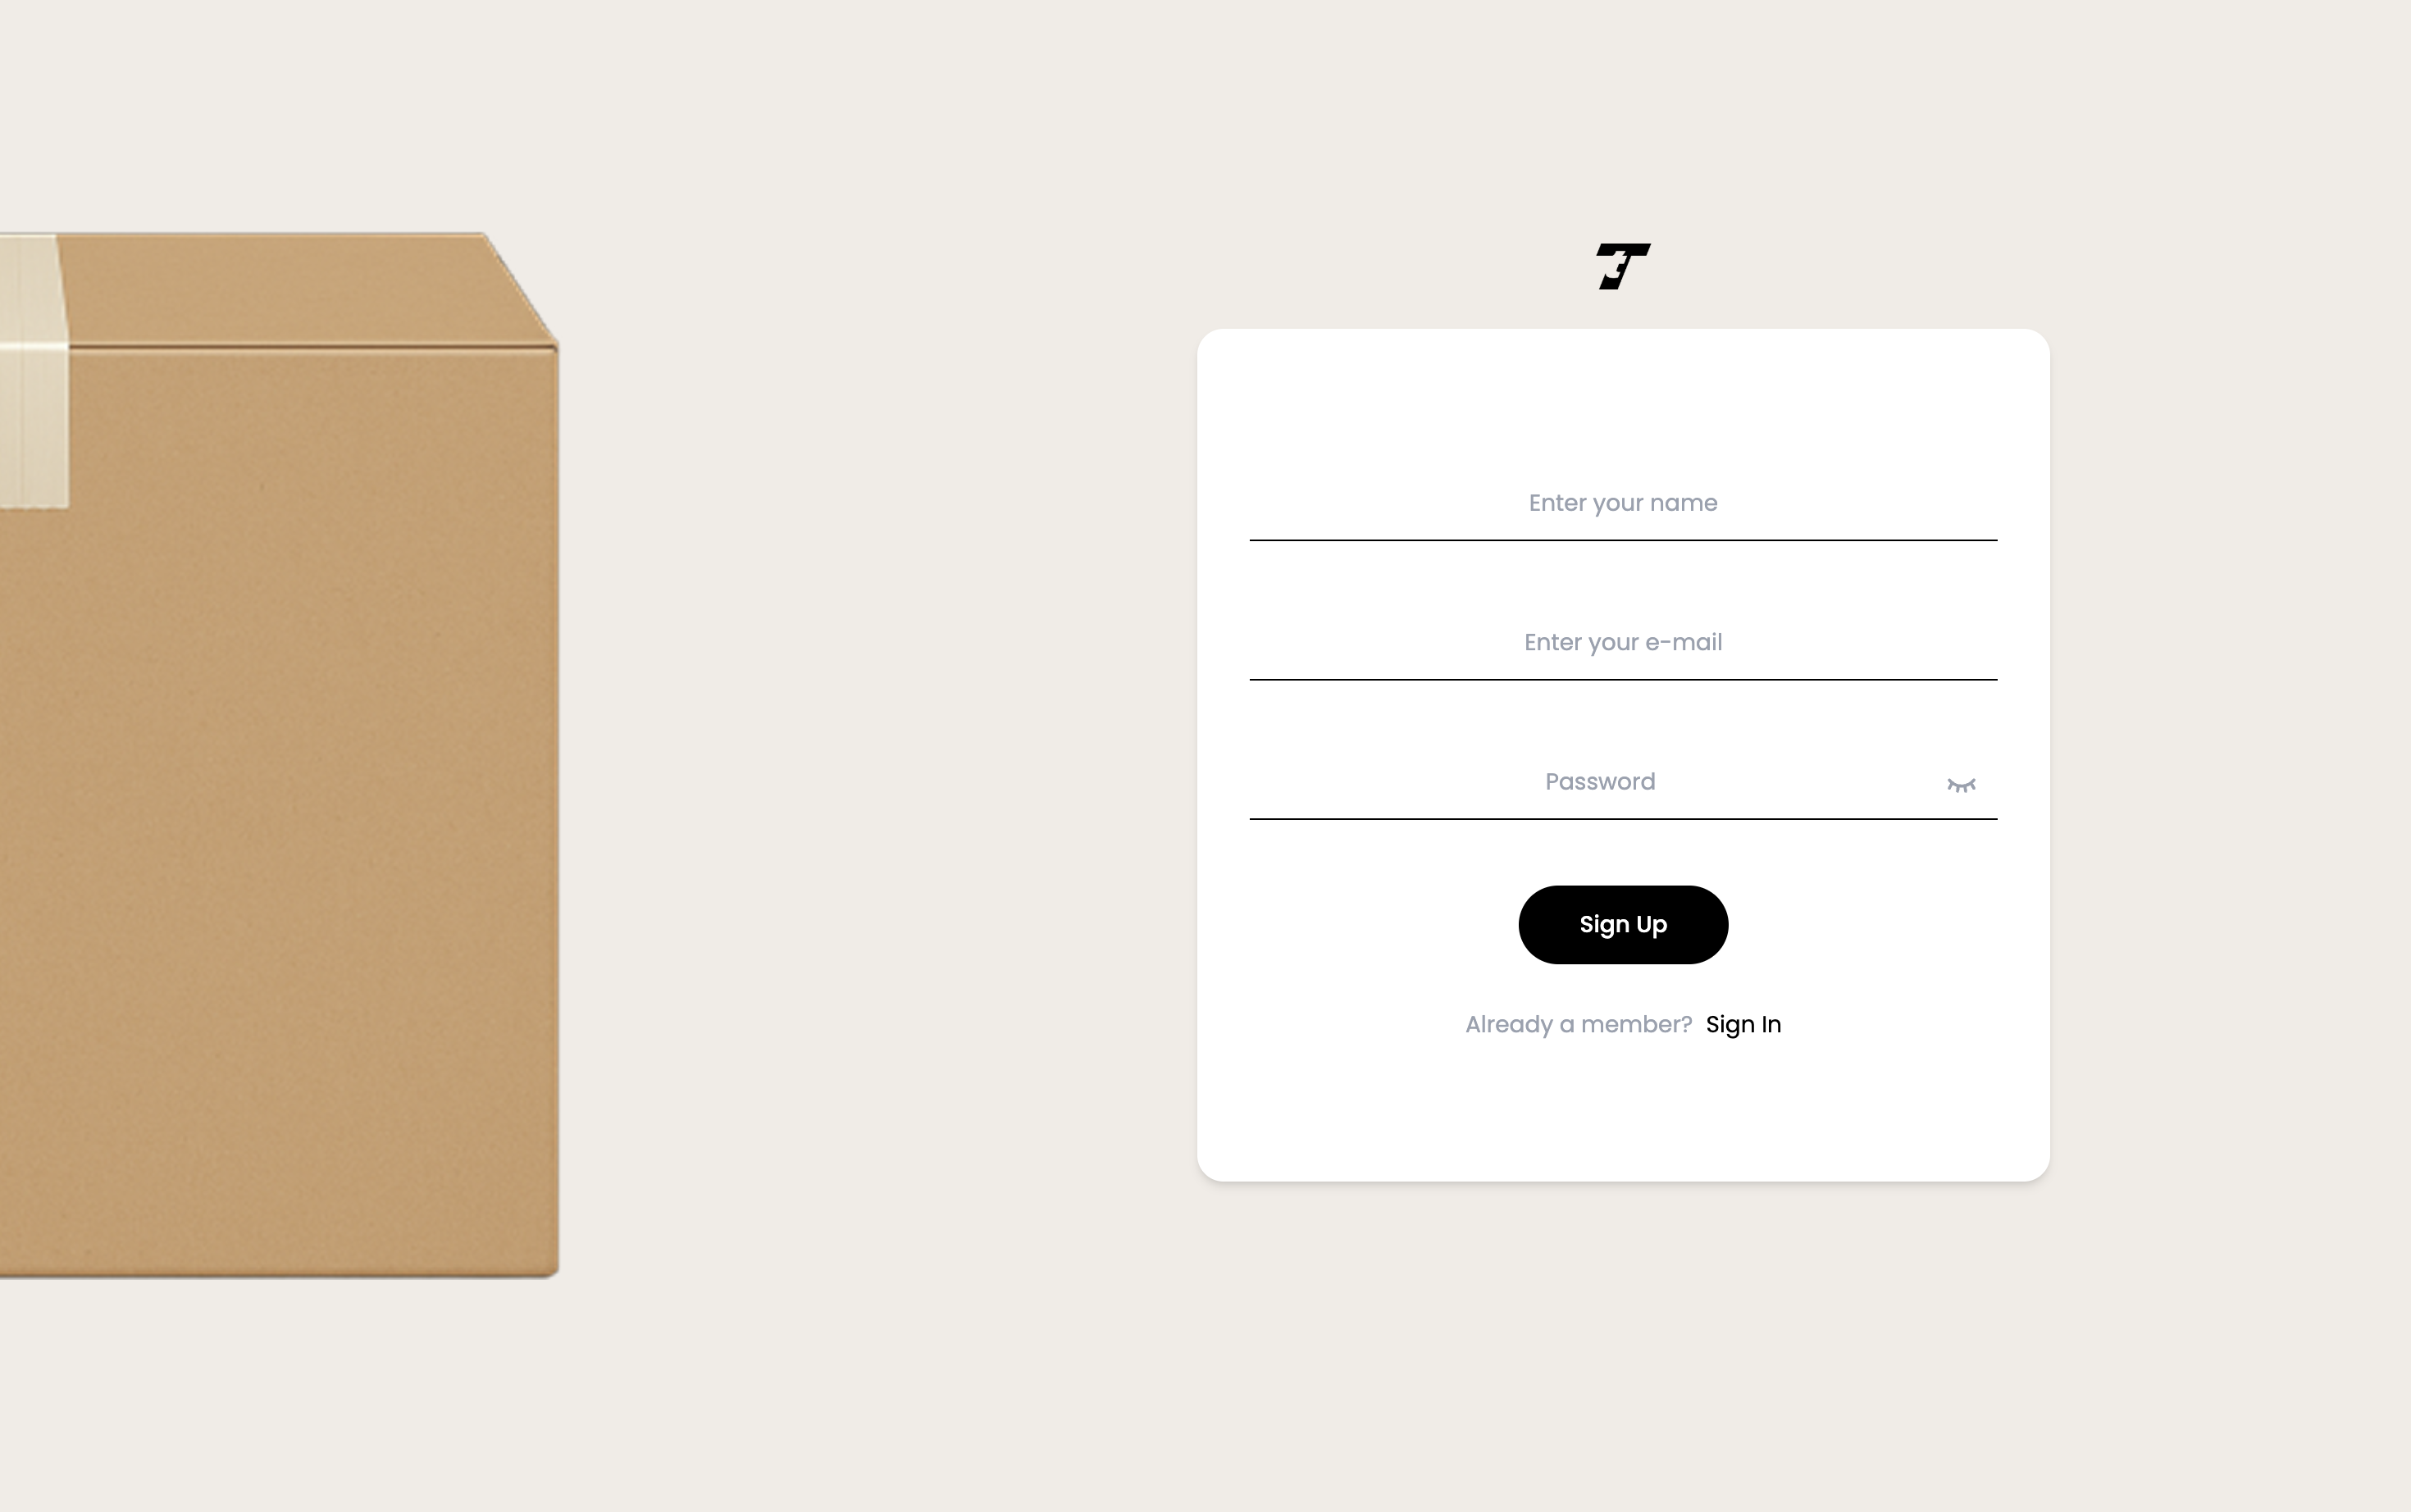
\includegraphics[width=0.8\textwidth]{signup.png}
    \caption{หน้าสมัครสมาชิก}
    \label{fig:ui_signup}
\end{figure}
\end{minipage}


\subsection{ส่วนของผู้ใช้งานทั่วไป}
หมวดหมู่นี้ถูกออกแบบมาเพื่อรองรับผู้ใช้งานใน 2 บทบาทหลัก ได้แก่ \textbf{ผู้ส่งพัสดุ (Sender)} ซึ่งเป็นผู้เดียวที่มีสิทธิ์ในการกรอกและจัดการข้อมูลการจัดส่ง และ \textbf{ผู้ใช้งานทั่วไปหรือผู้รับพัสดุ (Recipient)} ที่เน้นการติดตามสถานะและตรวจสอบความถูกต้อง โดยมีหน้าต่างการทำงานดังนี้:

\vspace{1em}
\begin{minipage}{\linewidth}
\noindent \textbf{1. หน้ากรอกข้อมูลผู้ส่ง} \\
สำหรับให้ \textbf{ผู้ส่งพัสดุ} บันทึกข้อมูลส่วนตัวและที่อยู่ของตนเอง \textit{(ผู้ใช้งานทั่วไปในบทบาทอื่นจะไม่สามารถกรอกข้อมูลในส่วนนี้ได้)}
\begin{figure}[H]
    \centering
    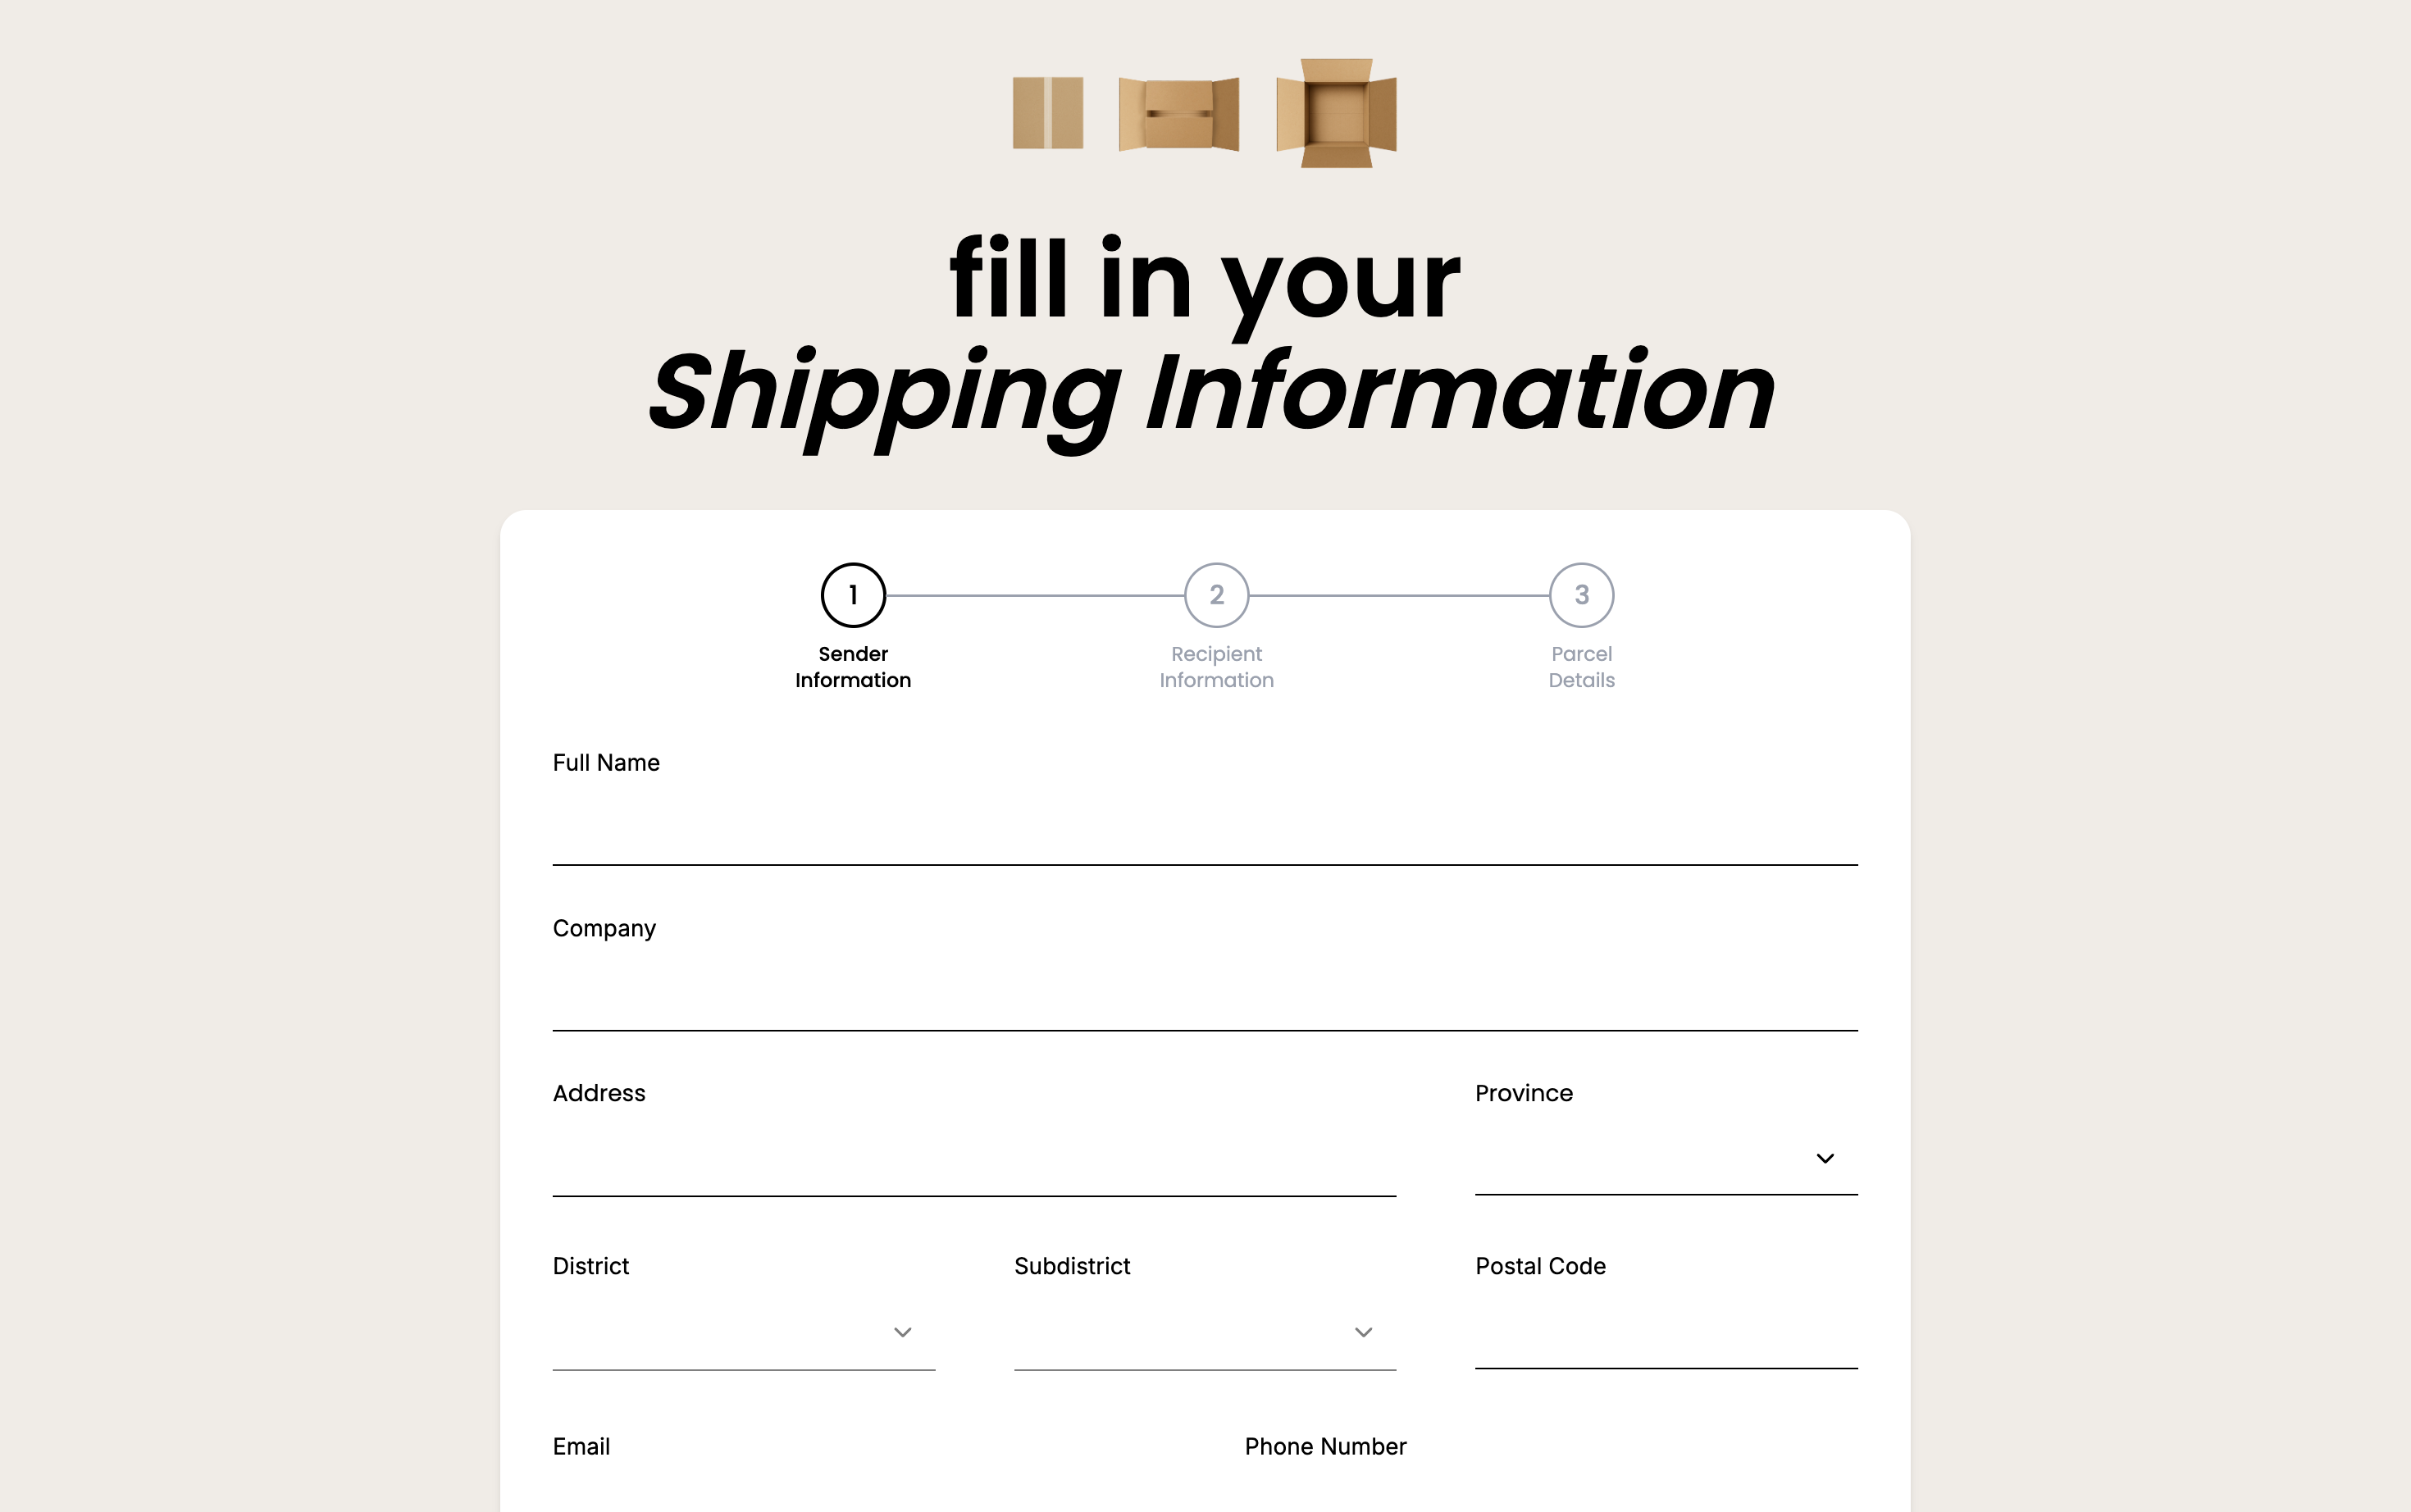
\includegraphics[width=0.8\textwidth]{fillsenderaddress.png}
    \caption{หน้ากรอกข้อมูลผู้ส่ง}
    \label{fig:ui_user_sender}
\end{figure}
\end{minipage}

\vspace{1em}
\begin{minipage}{\linewidth}
\noindent \textbf{2. หน้ากรอกรายละเอียดพัสดุ} \\
สำหรับให้ \textbf{ผู้ส่งพัสดุ} ระบุข้อมูลสำคัญของสินค้า เช่น น้ำหนัก ขนาด และช่วงอุณหภูมิควบคุมที่ต้องการ
\begin{figure}[H]
    \centering
    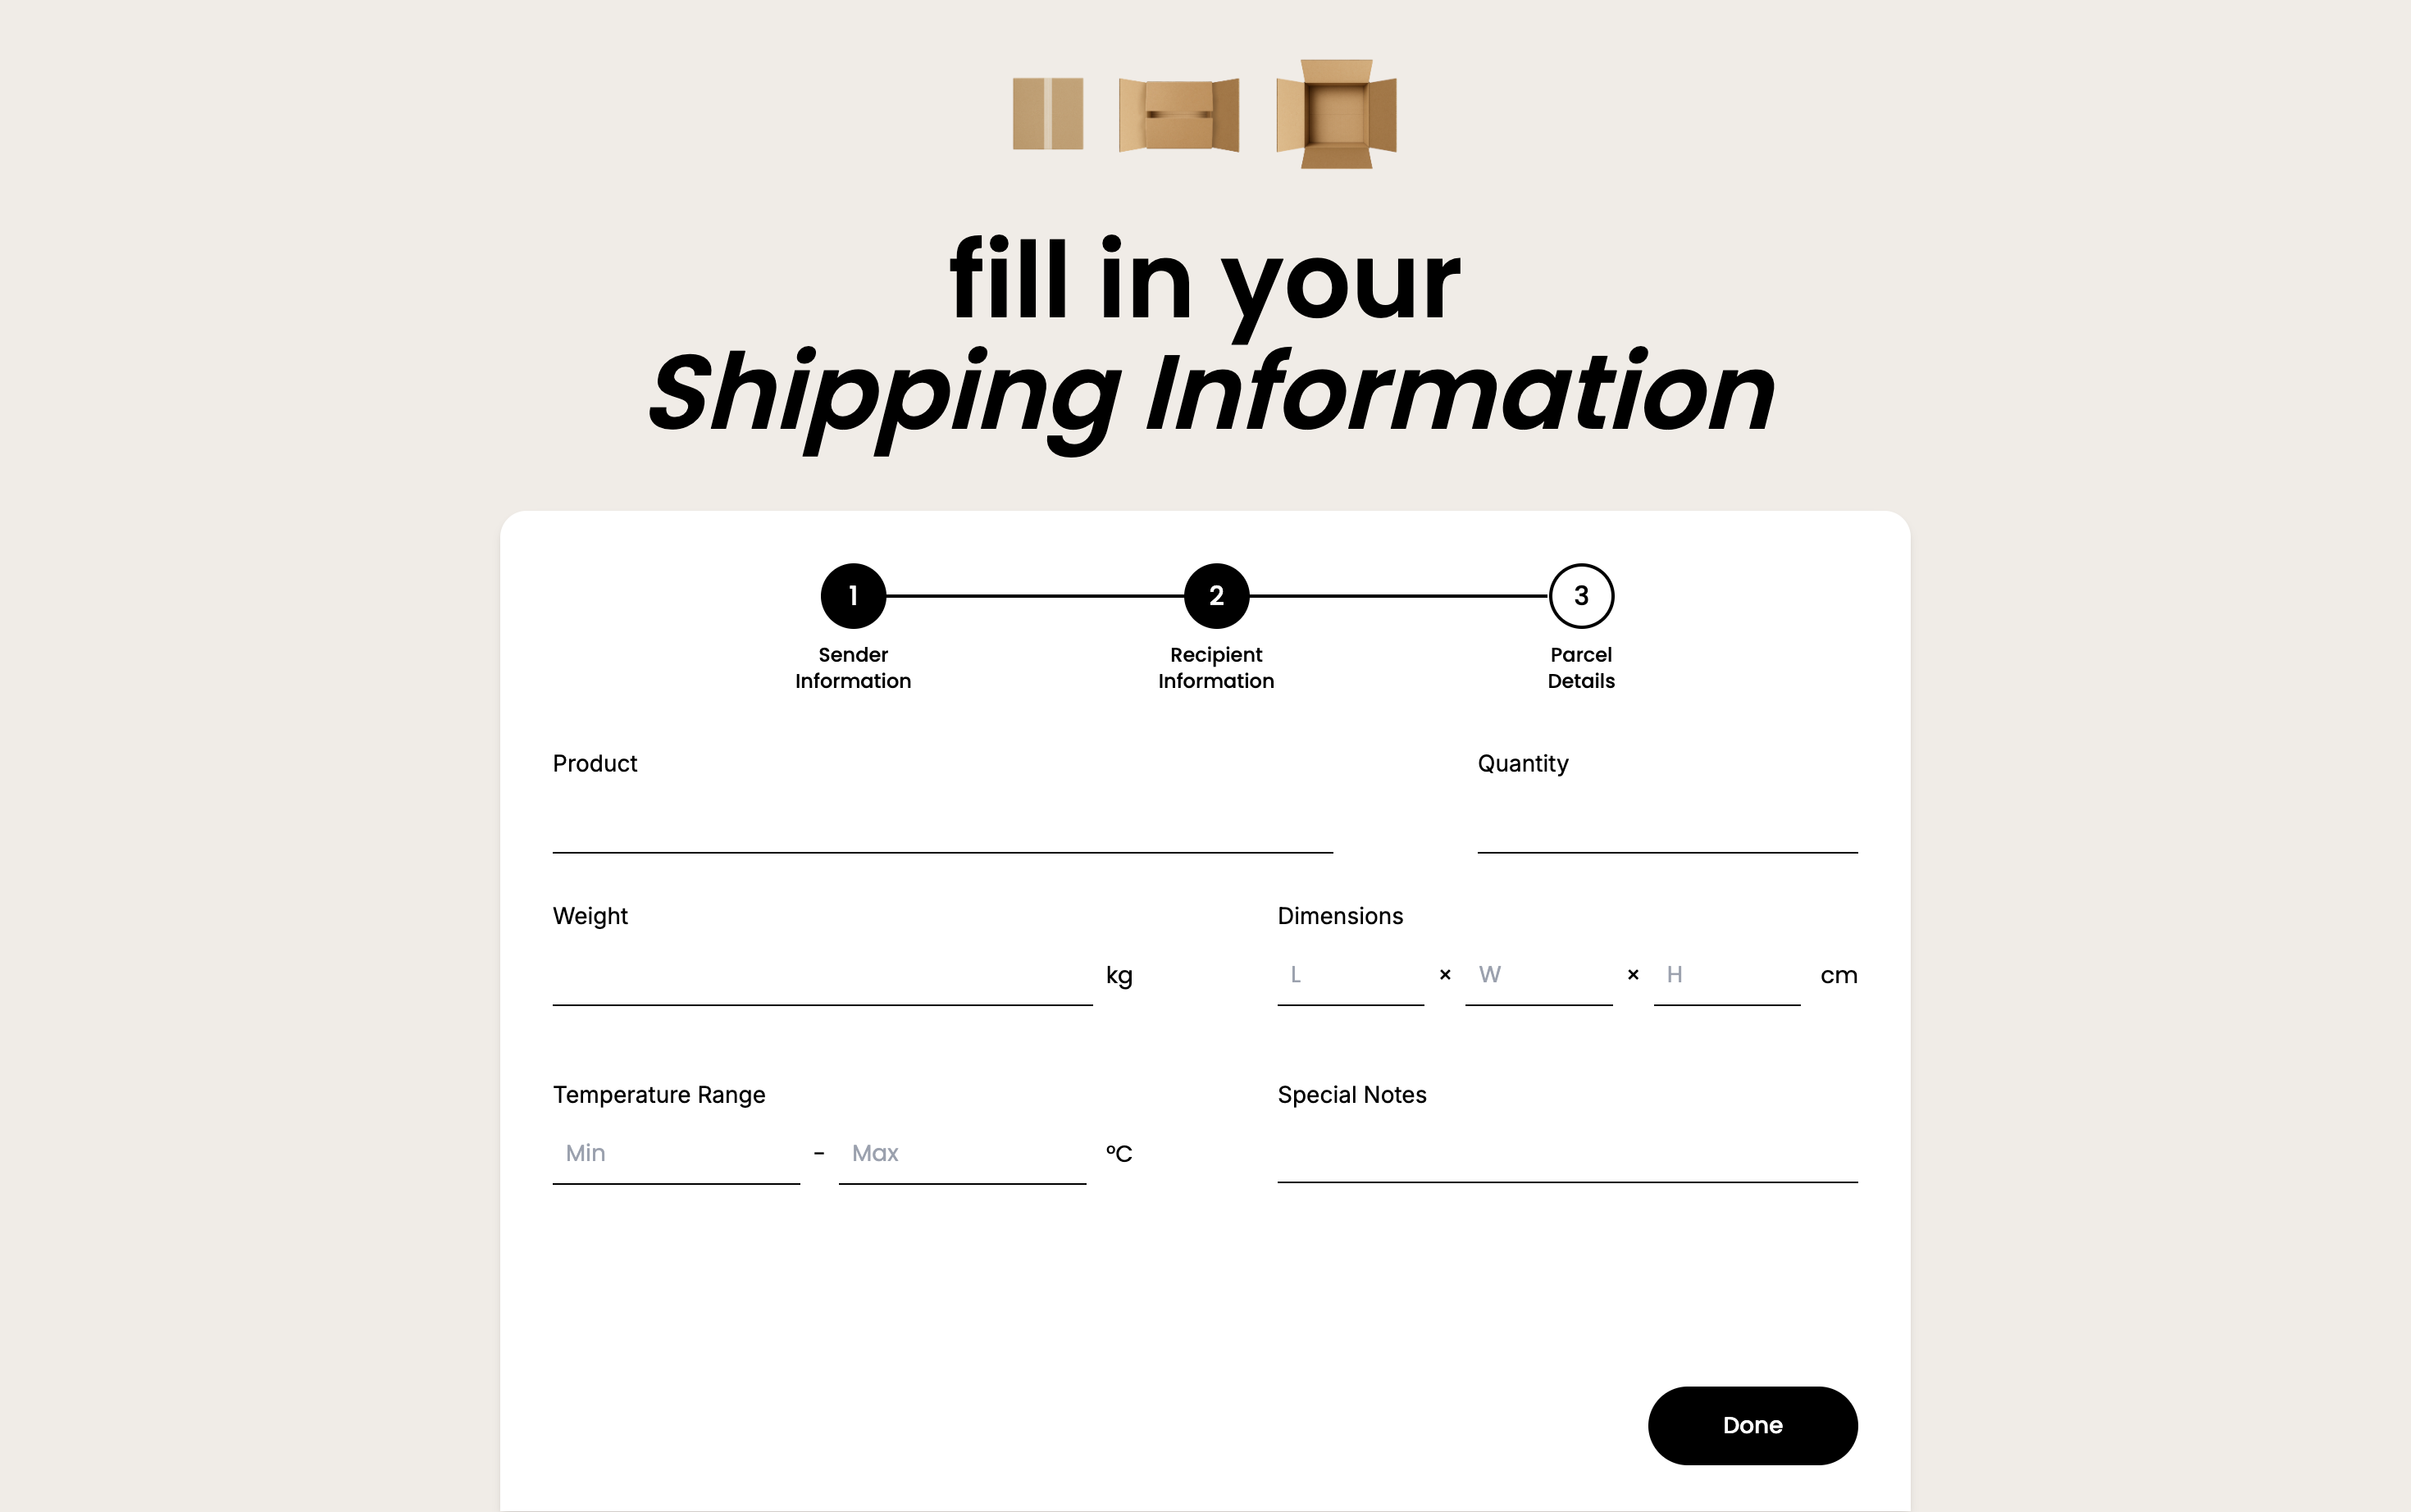
\includegraphics[width=0.8\textwidth]{fillparceldetail.png}
    \caption{หน้ากรอกรายละเอียดพัสดุ}
    \label{fig:ui_user_parcel}
\end{figure}
\end{minipage}

\vspace{1em}
\begin{minipage}{\linewidth}
\noindent \textbf{3. หน้ากรอกข้อมูลผู้รับ} \\
สำหรับให้ \textbf{ผู้ส่งพัสดุ} บันทึกที่อยู่และช่องทางการติดต่อของปลายทาง
\begin{figure}[H]
    \centering
    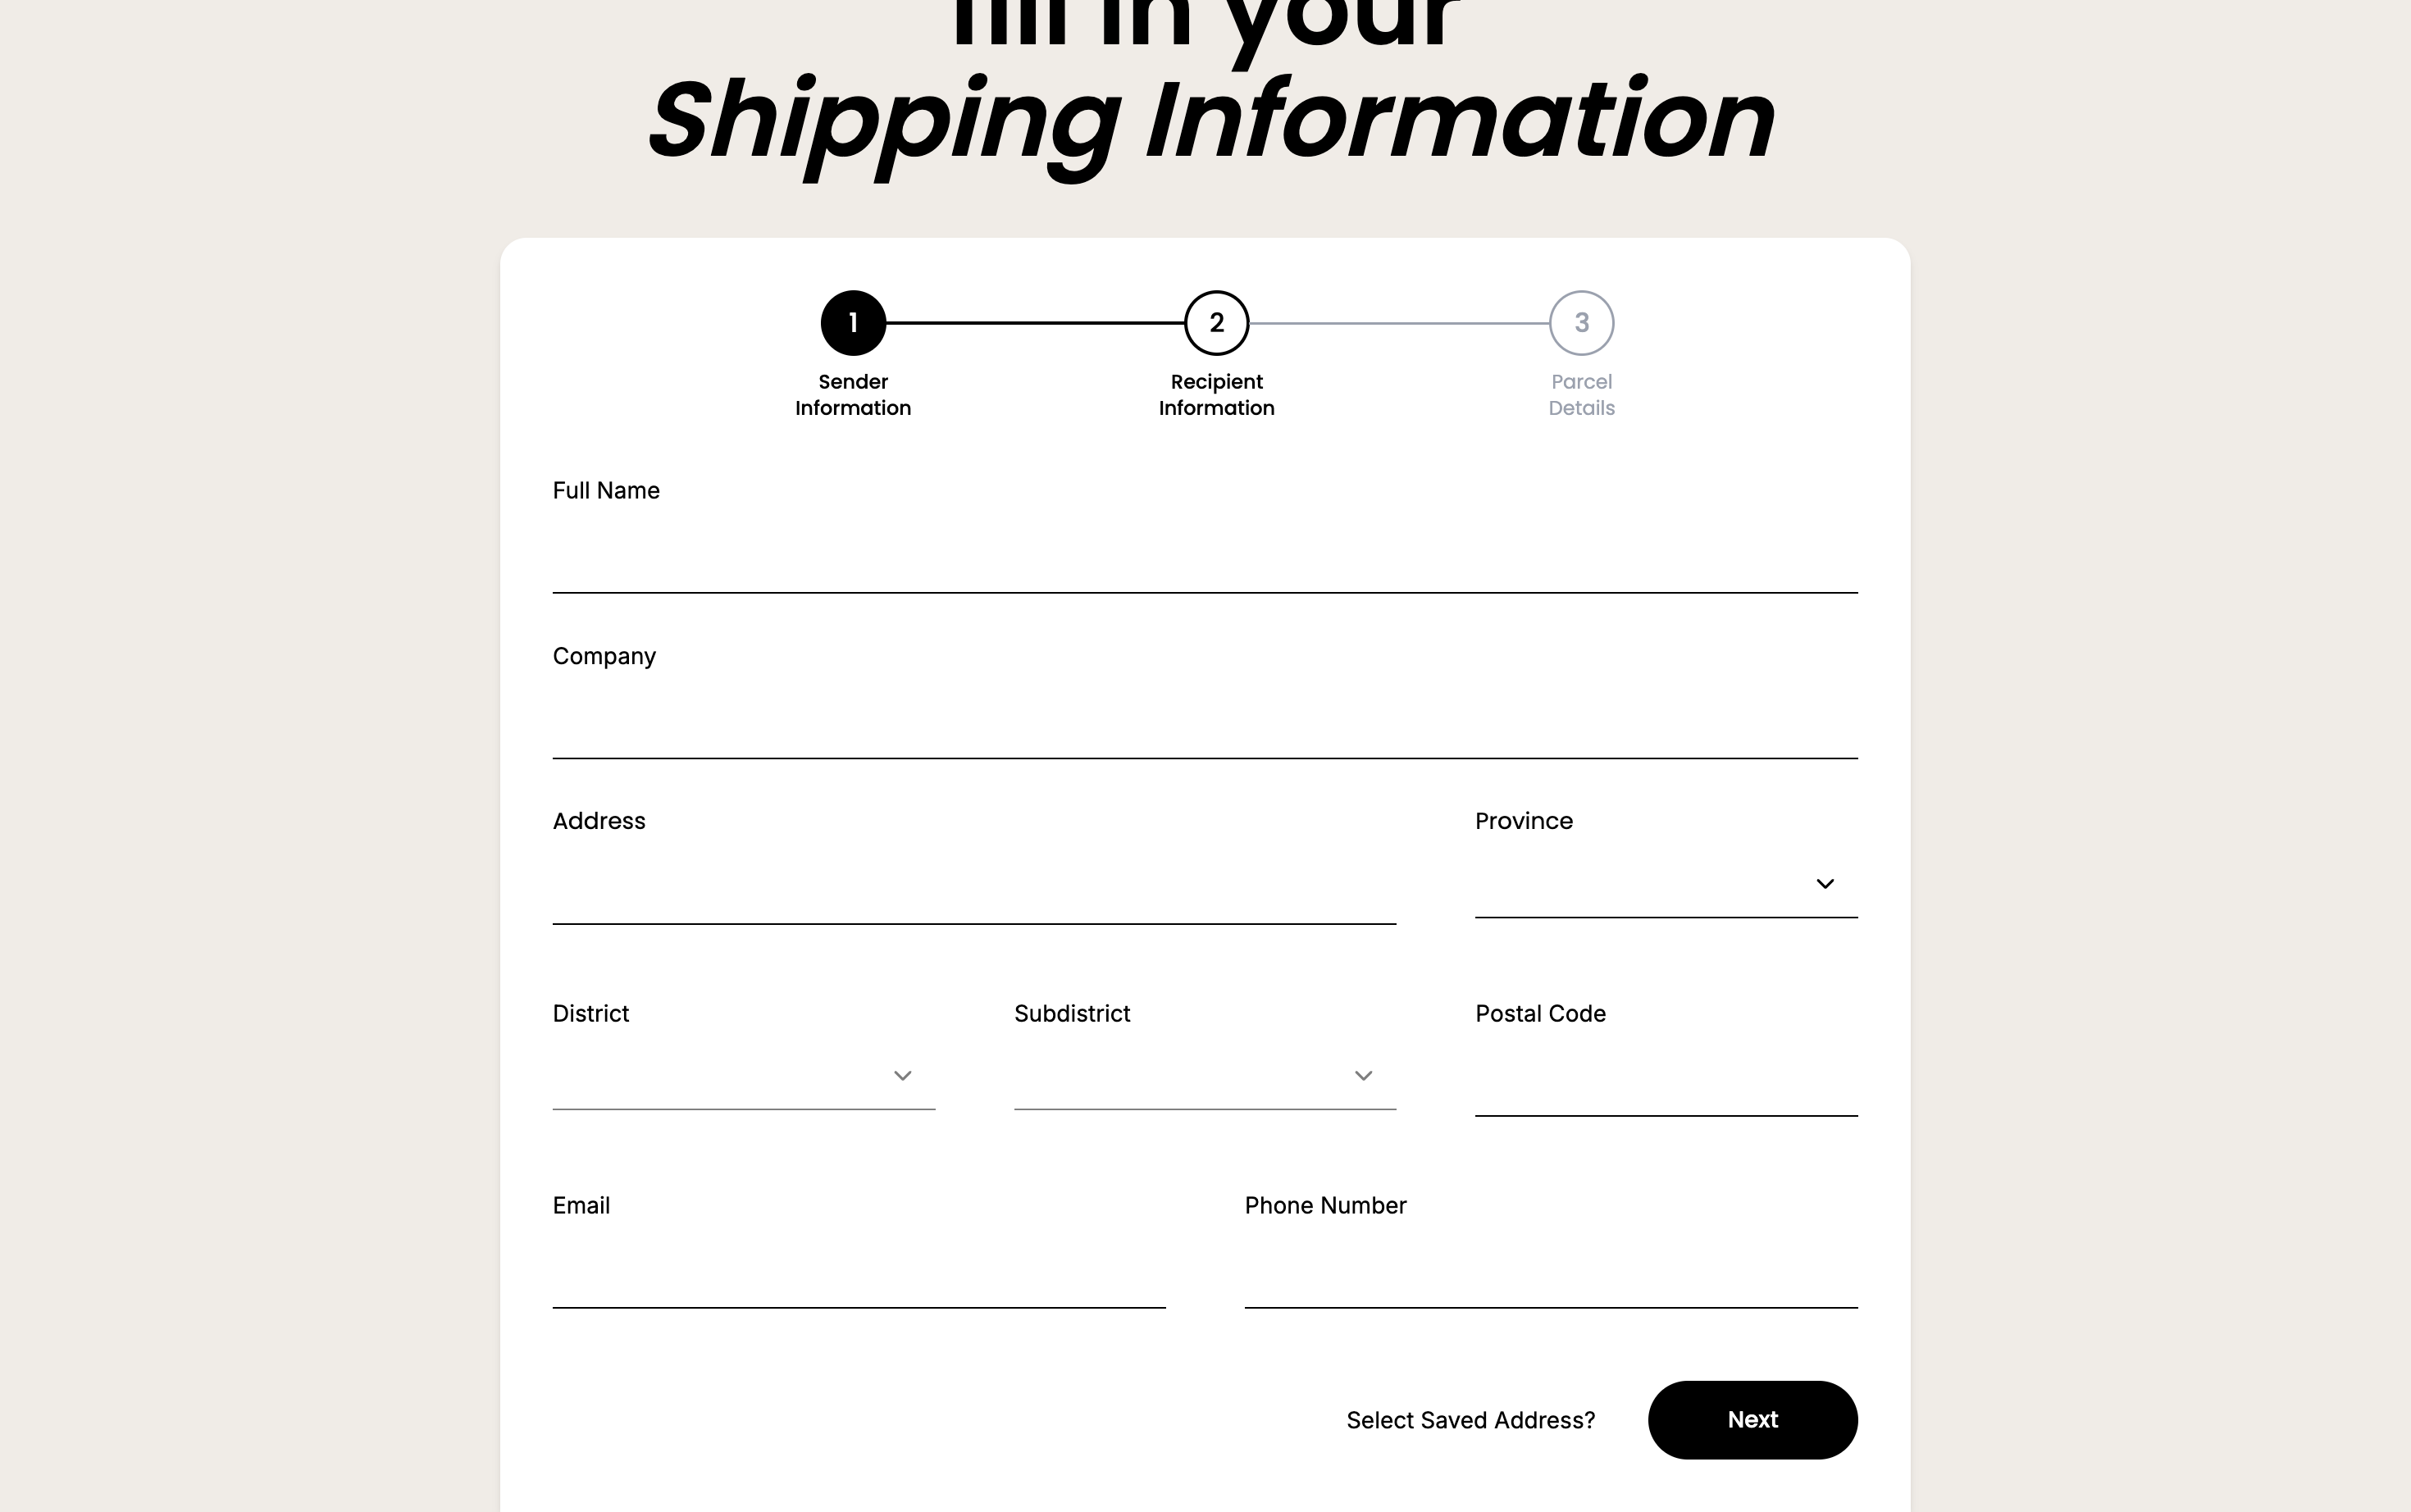
\includegraphics[width=0.8\textwidth]{fillrecipientaddress.png}
    \caption{หน้ากรอกข้อมูลผู้รับ}
    \label{fig:ui_user_recipient}
\end{figure}
\end{minipage}

\vspace{1em}
\begin{minipage}{\linewidth}
\noindent \textbf{4. หน้าเพิ่มที่อยู่จัดส่ง} \\
สำหรับให้ \textbf{ผู้ส่งพัสดุ} บันทึกข้อมูลที่อยู่ผู้ส่งหรือผู้รับรายการใหม่เข้าสู่ระบบ เพื่อความสะดวกรวดเร็วในการจัดส่งครั้งต่อไป
\begin{figure}[H]
    \centering
    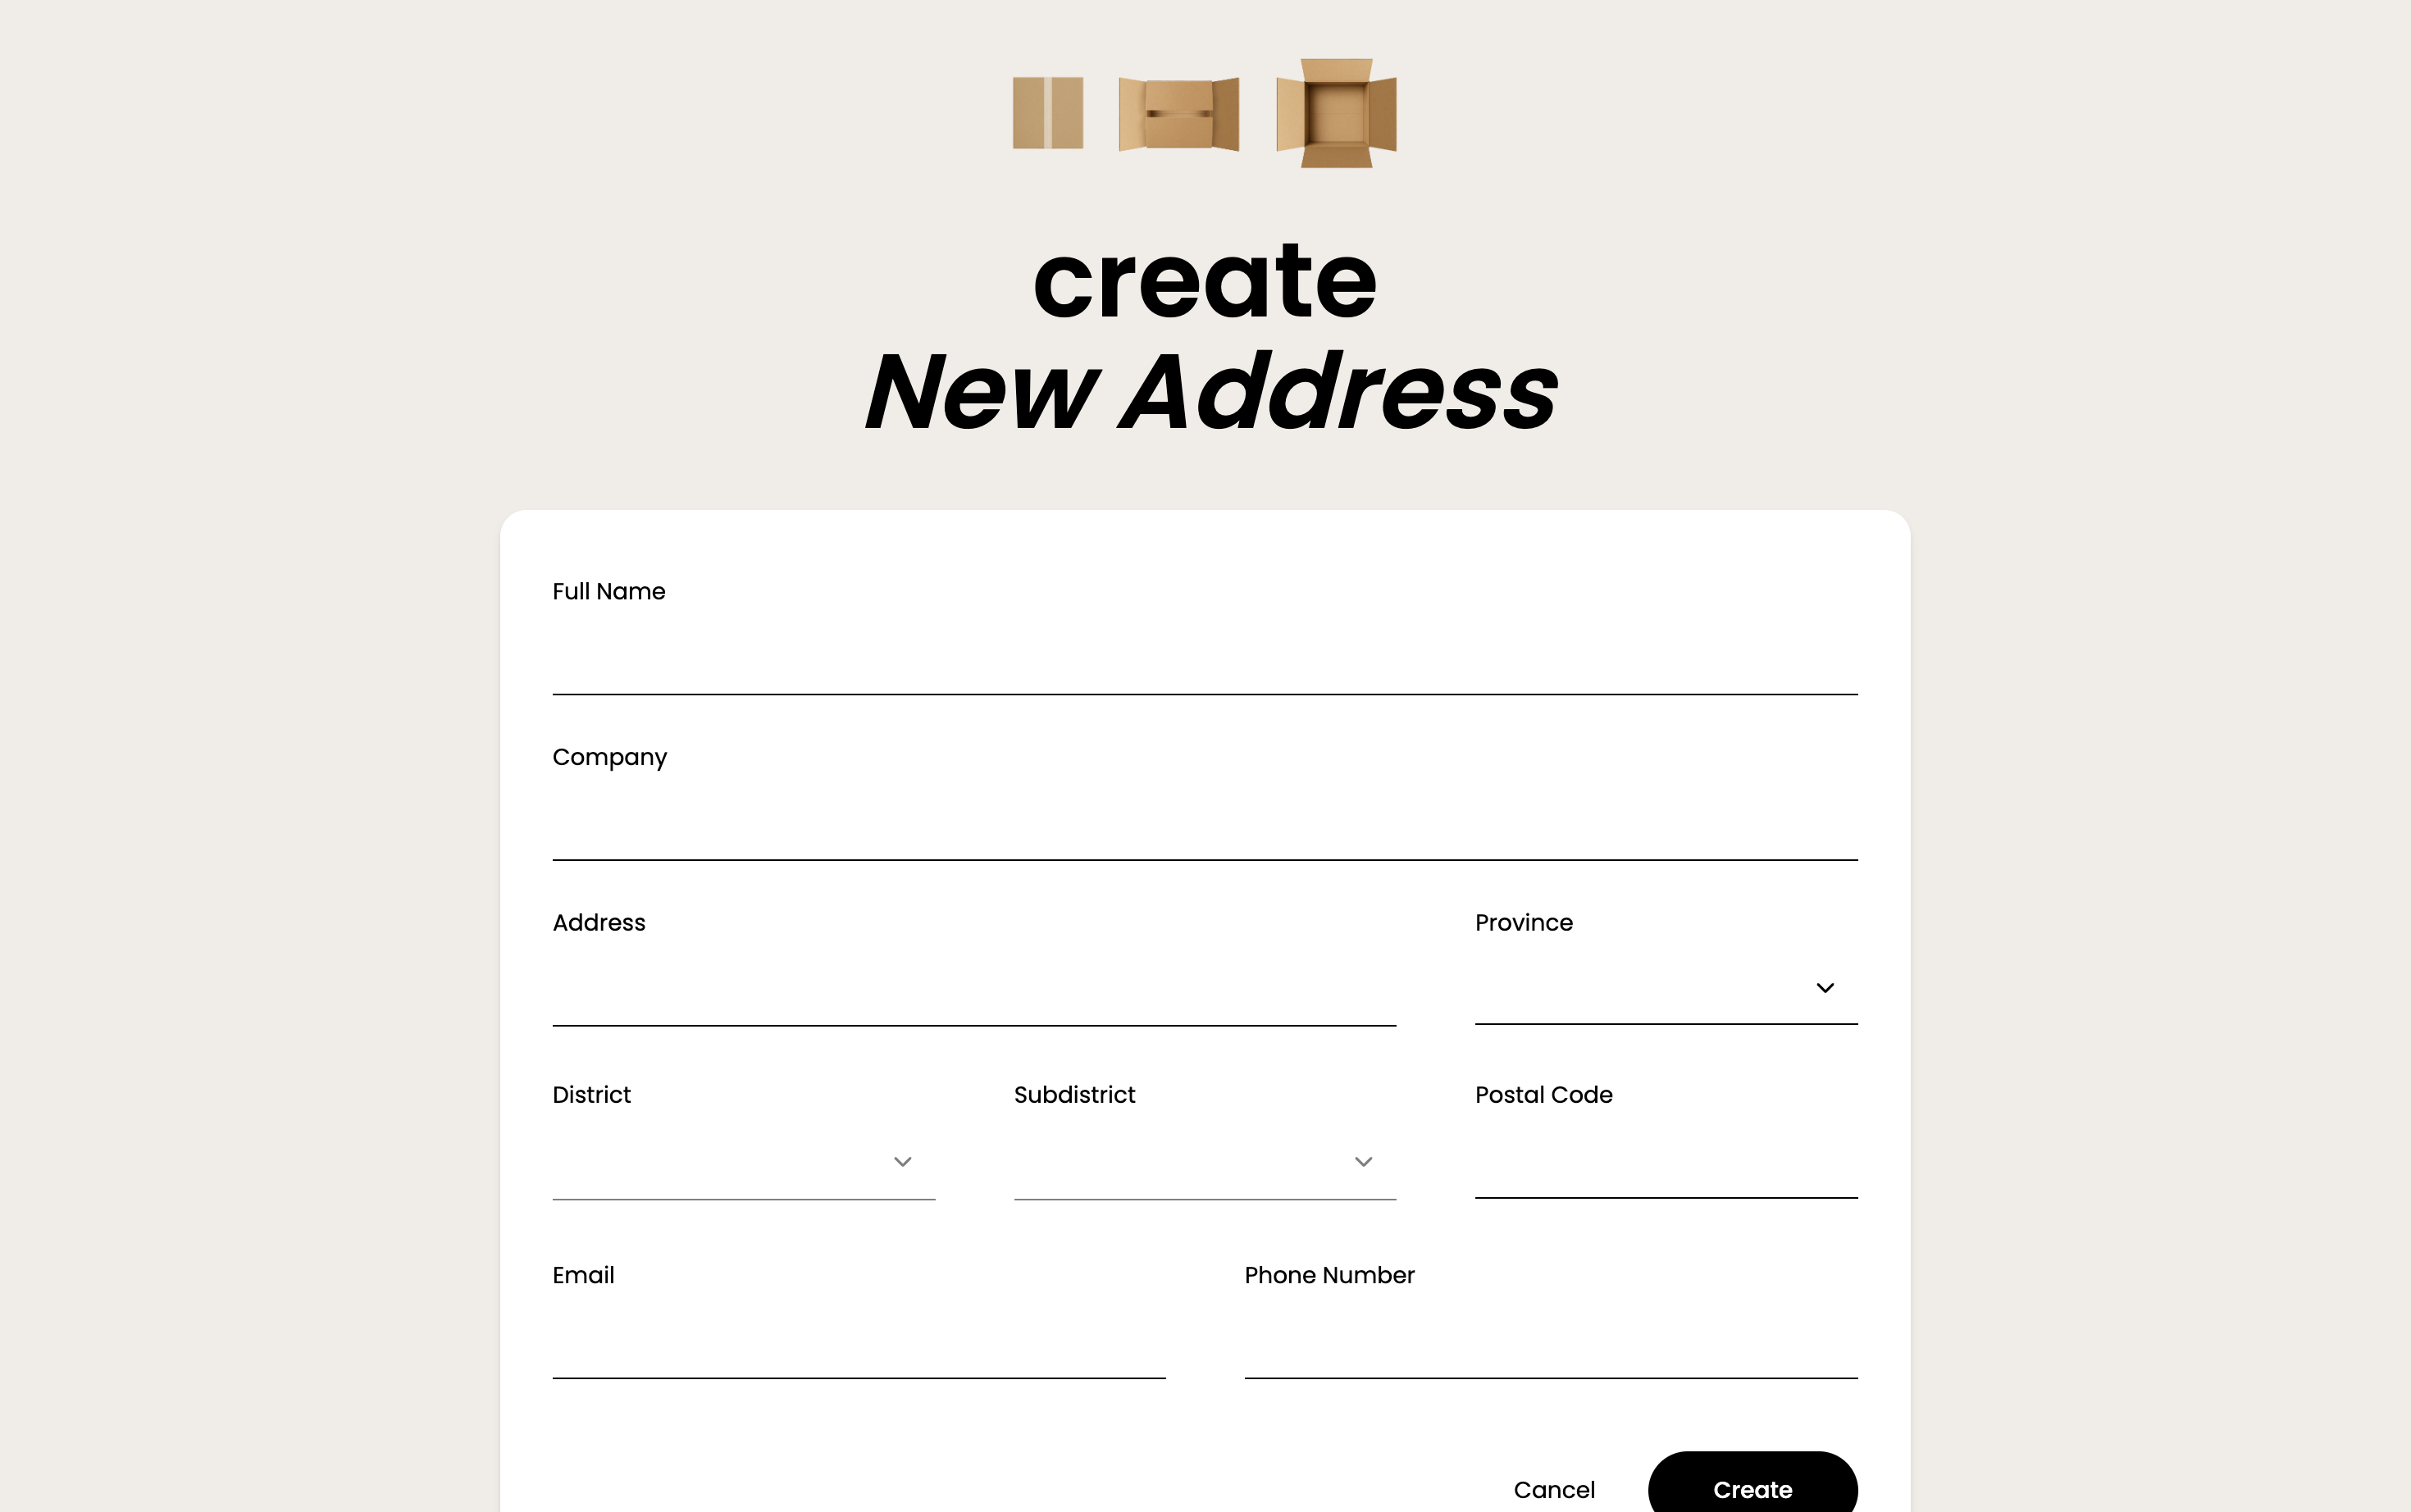
\includegraphics[width=0.8\textwidth]{addsavedaddress.png}
    \caption{หน้าเพิ่มที่อยู่จัดส่ง}
    \label{fig:ui_user_add_address}
\end{figure}
\end{minipage}

\vspace{1em}
\begin{minipage}{\linewidth}
\noindent \textbf{5. หน้าจัดการที่อยู่จัดส่ง} \\
สำหรับให้ \textbf{ผู้ส่งพัสดุ} เรียกดู เลือกใช้งาน หรือแก้ไขข้อมูลที่อยู่ที่เคยถูกบันทึกไว้ในระบบ
\begin{figure}[H]
    \centering
    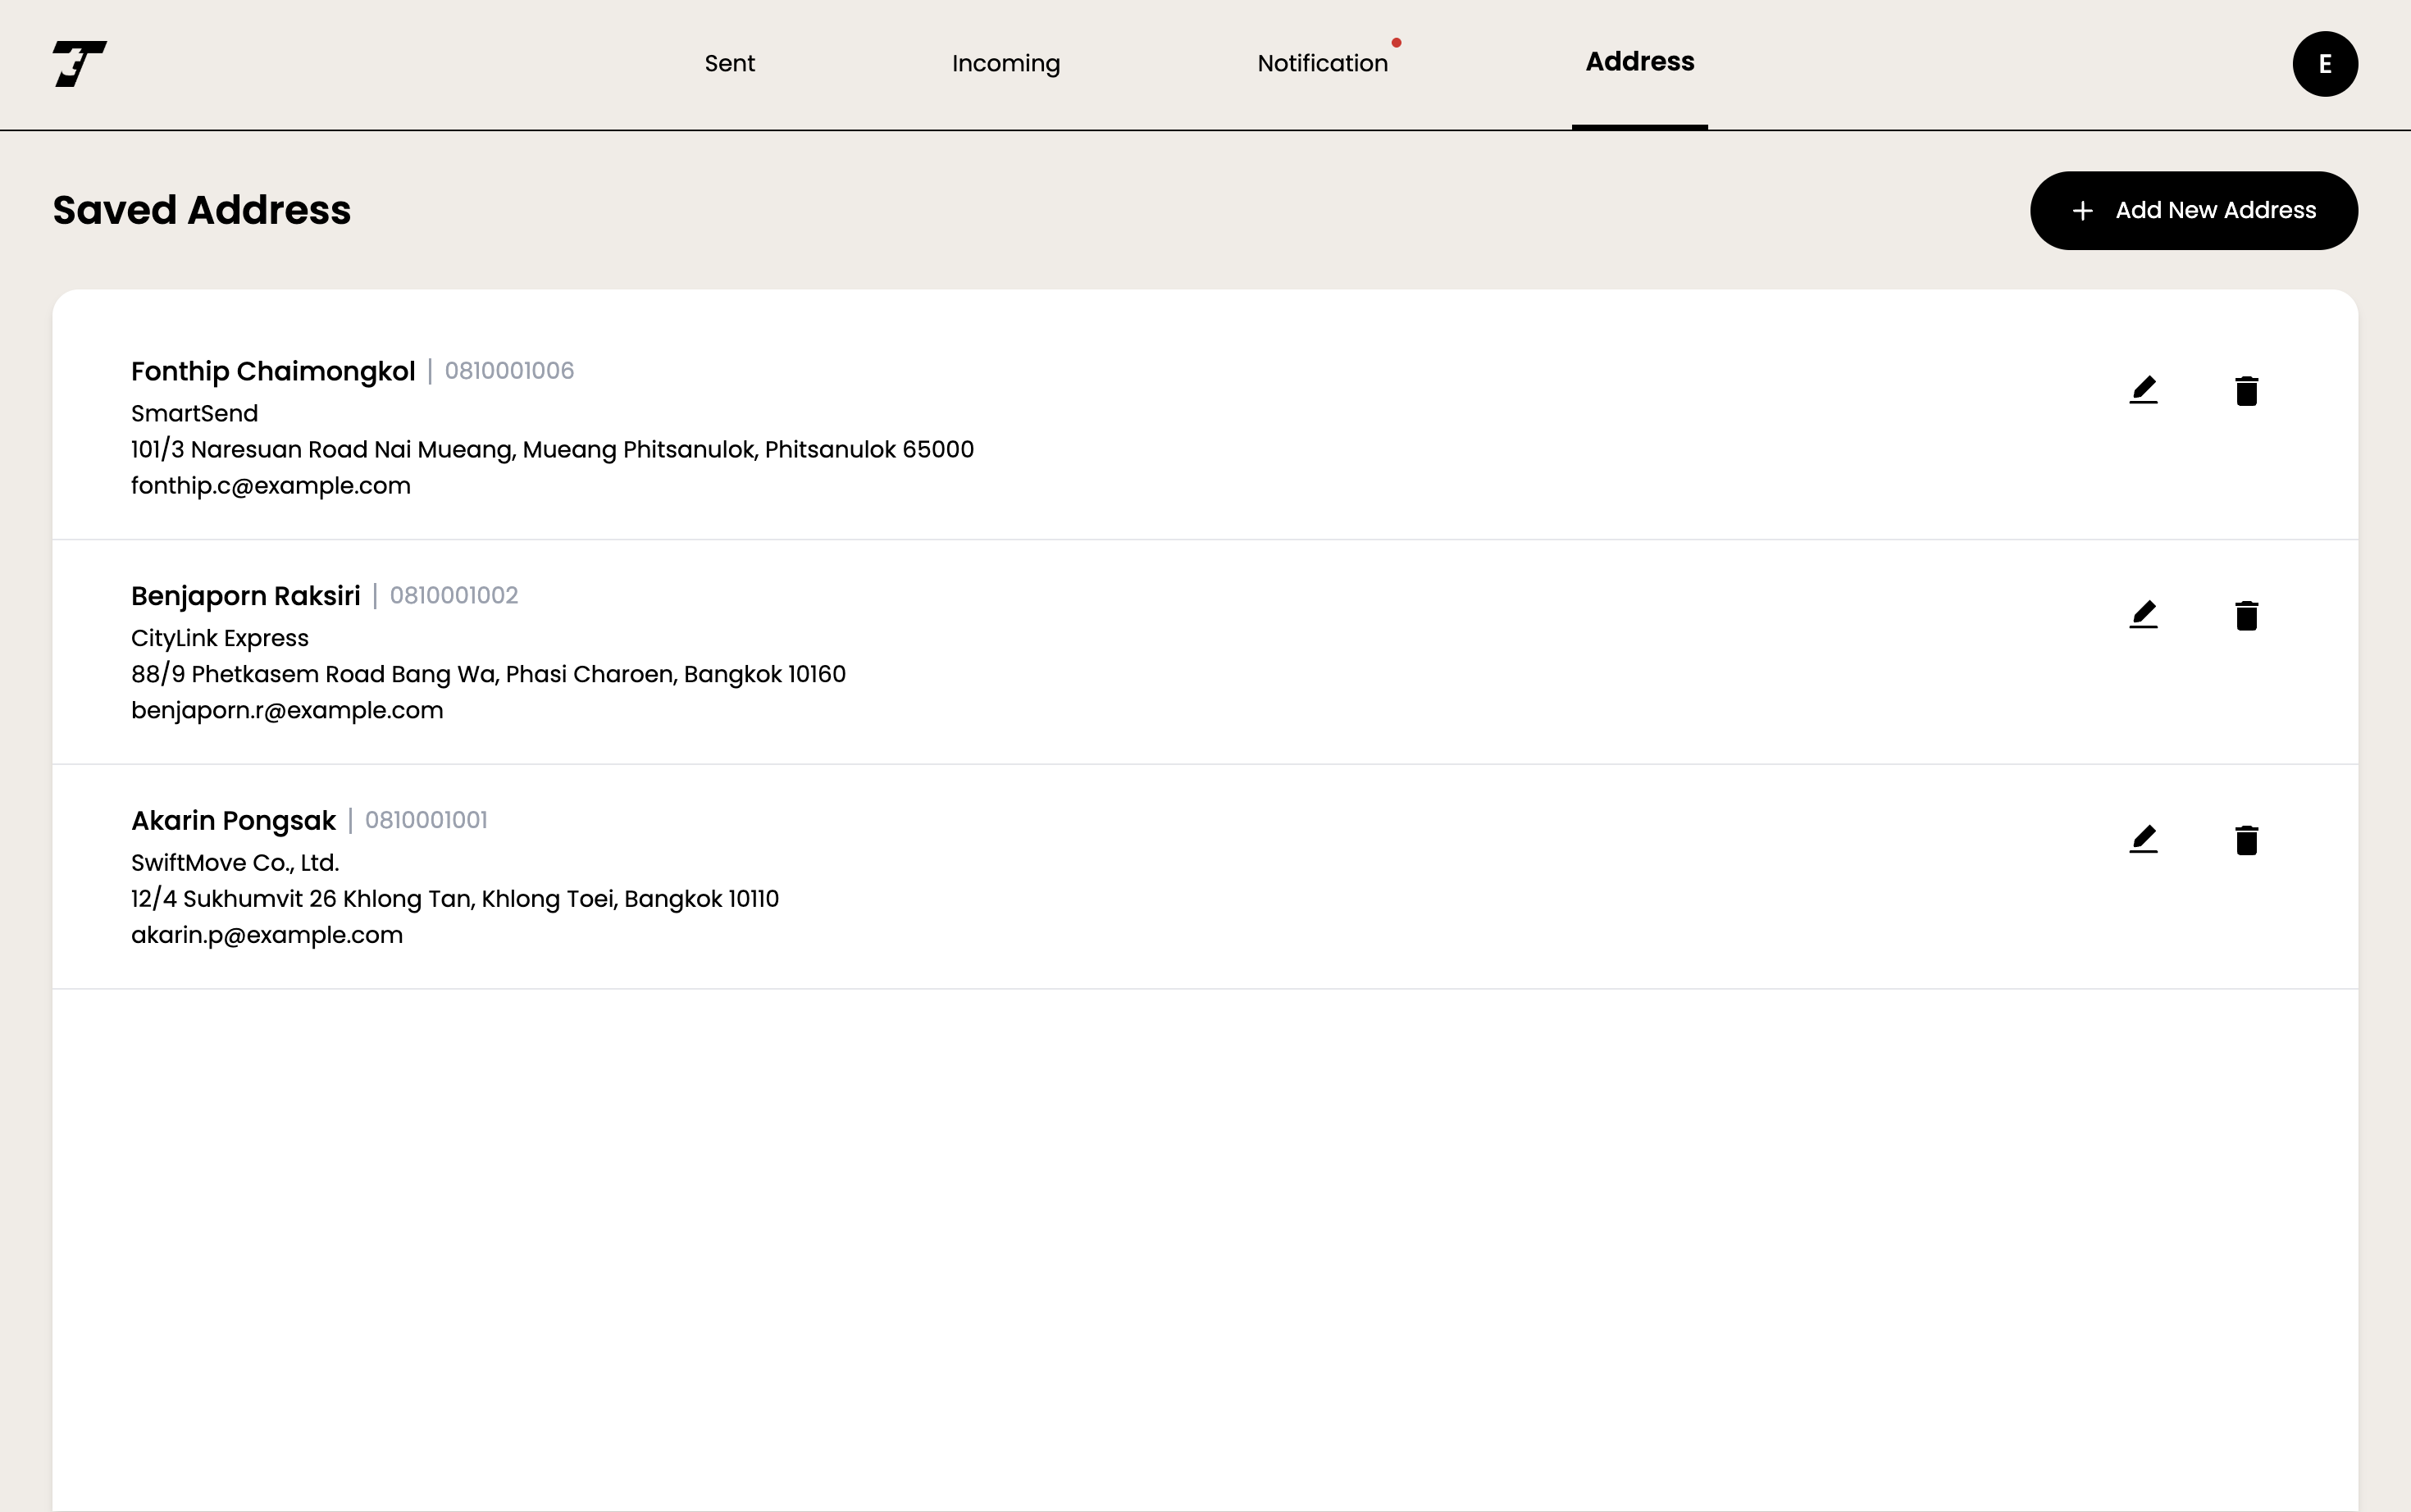
\includegraphics[width=0.8\textwidth]{savedaddress.png}
    \caption{หน้าจัดการที่อยู่จัดส่ง}
    \label{fig:ui_user_saved_address}
\end{figure}
\end{minipage}

\vspace{1em}
\begin{minipage}{\linewidth}
\noindent \textbf{6. หน้าตรวจสอบสถานะ} \\
สำหรับให้ \textbf{ผู้ใช้งานทั่วไปและผู้รับพัสดุ} สามารถกรอกหมายเลขติดตามพัสดุ เพื่อค้นหาสถานะการจัดส่ง
\begin{figure}[H]
    \centering
    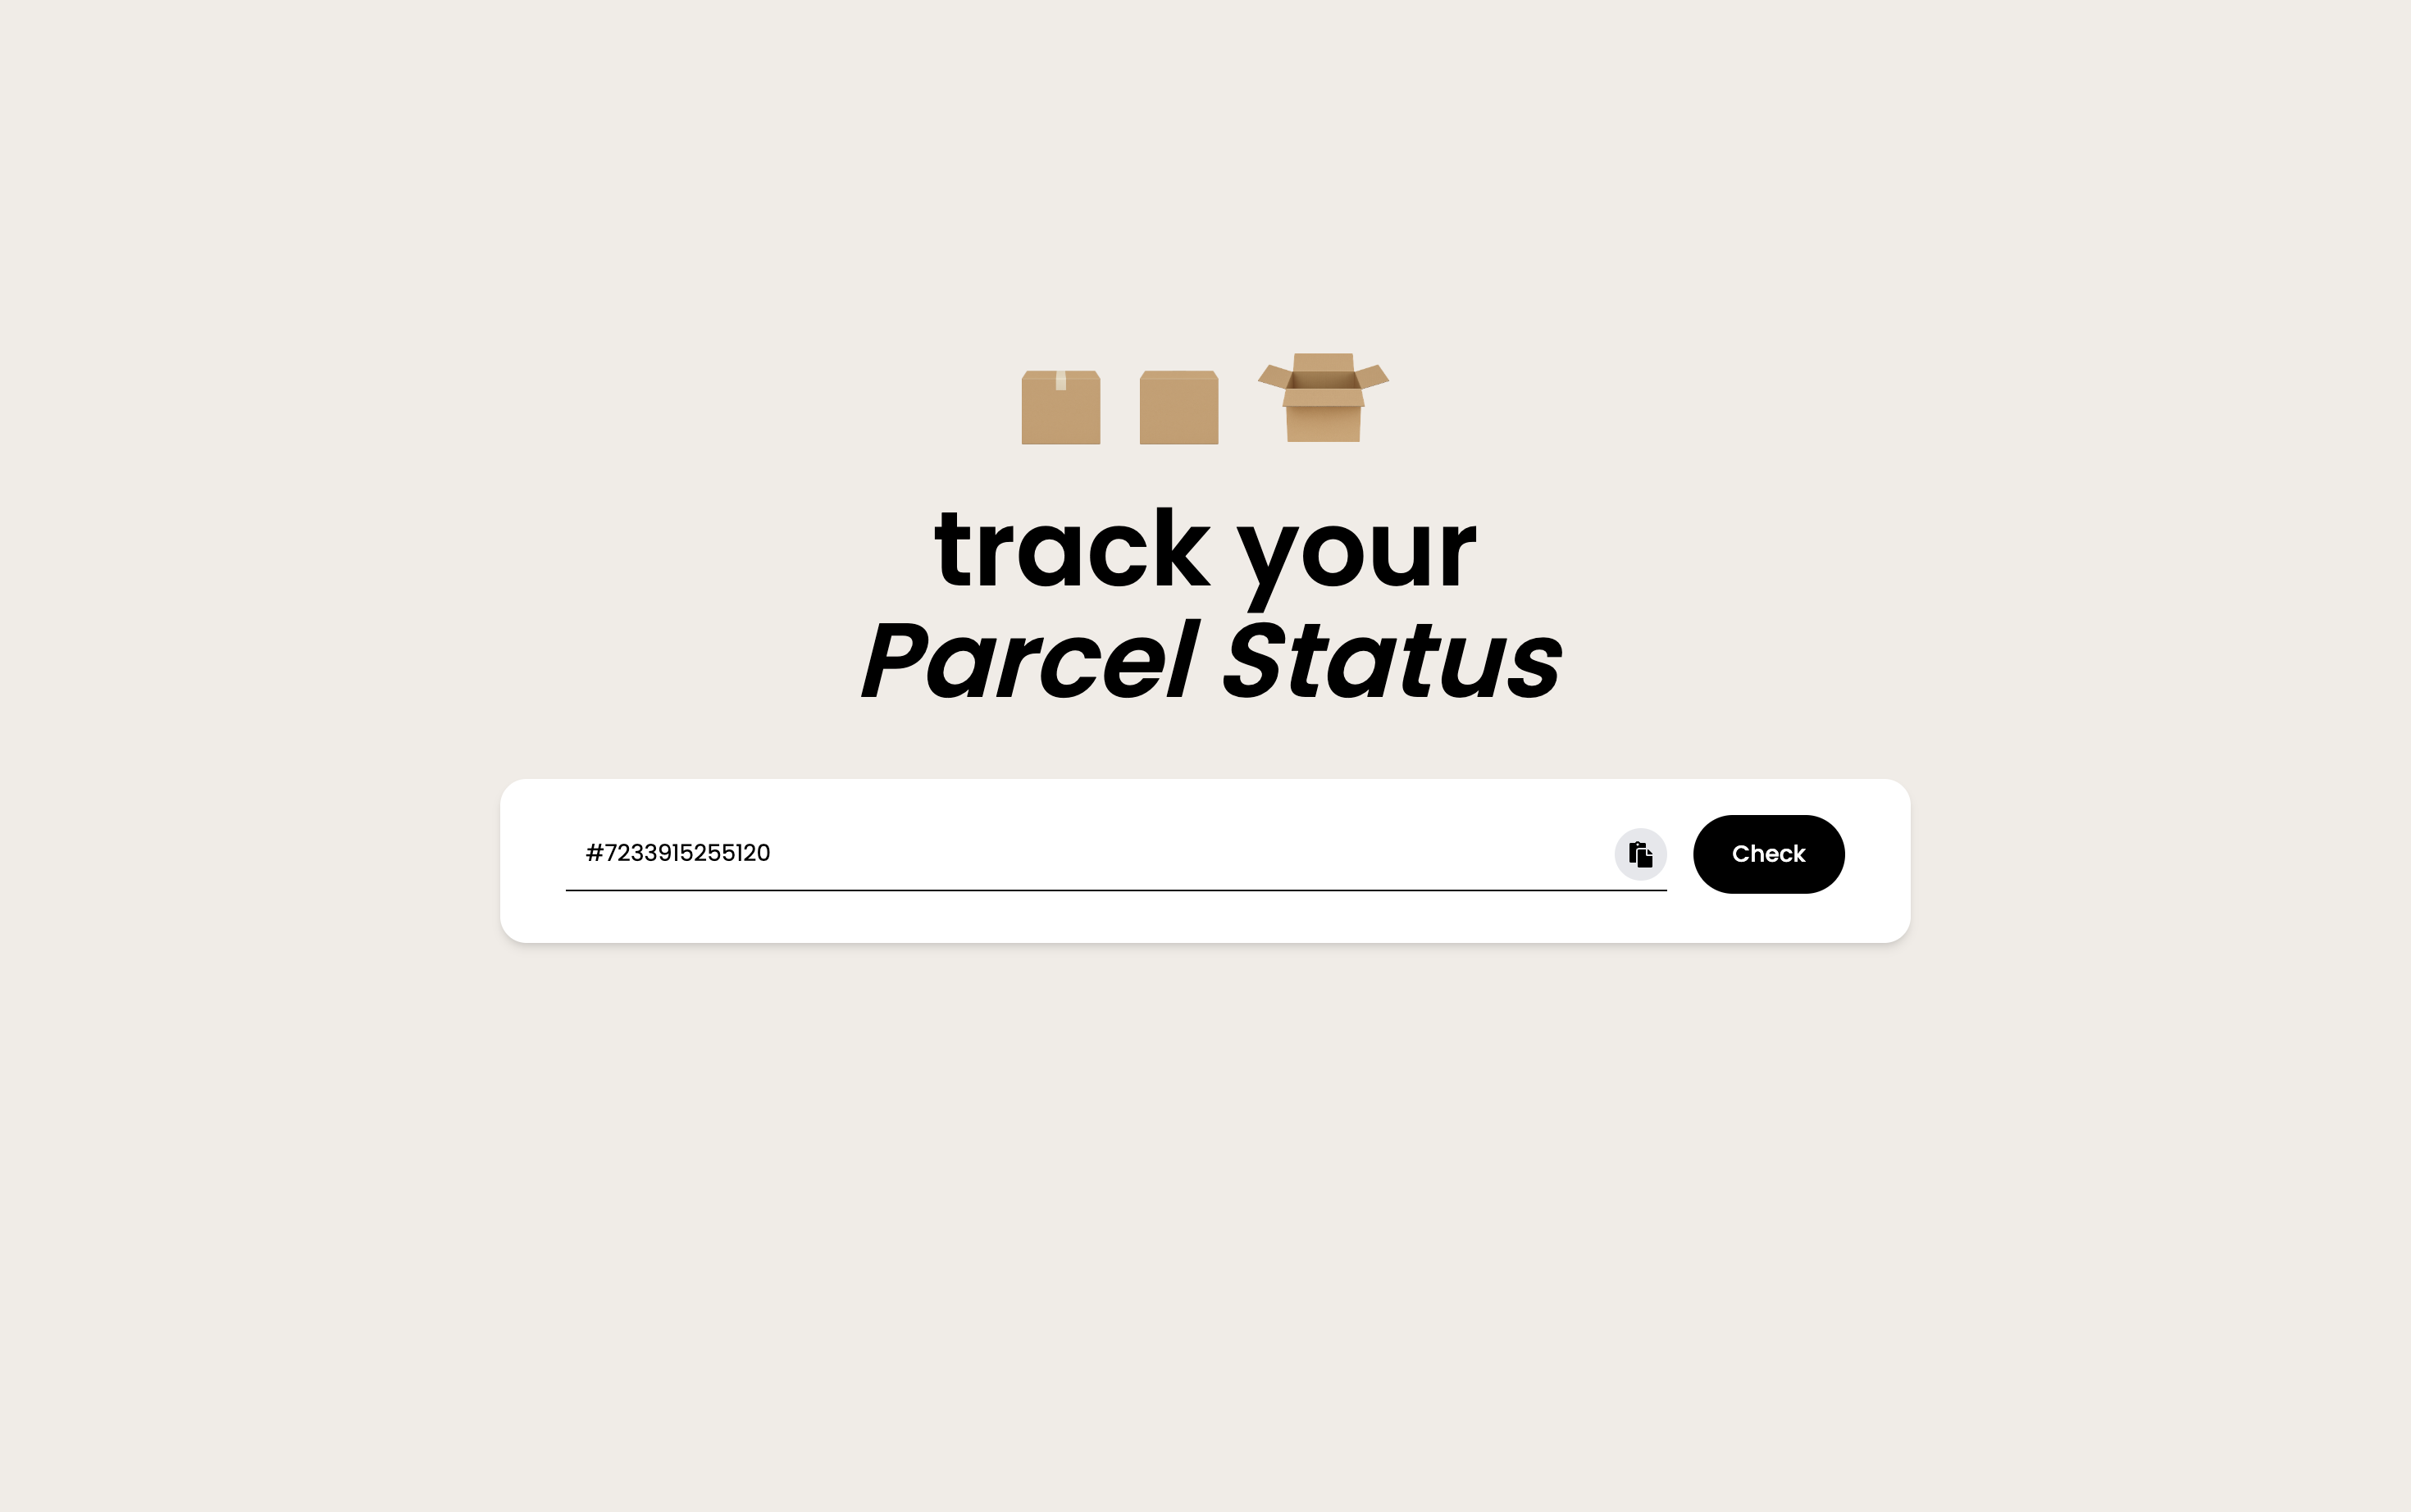
\includegraphics[width=0.8\textwidth]{checktracknum.png}
    \caption{หน้าตรวจสอบสถานะพัสดุ}
    \label{fig:ui_user_track}
\end{figure}
\end{minipage}

\vspace{1em}
\begin{minipage}{\linewidth}
\noindent \textbf{7. หน้ากระดานสรุปผลรายการที่กำลังจัดส่ง} \\
สำหรับให้ \textbf{ผู้รับพัสดุ} ดูสถานะและติดตามพัสดุที่กำลังอยู่ในระหว่างการจัดส่งไปยังจุดหมายปลายทาง
\begin{figure}[H]
    \centering
    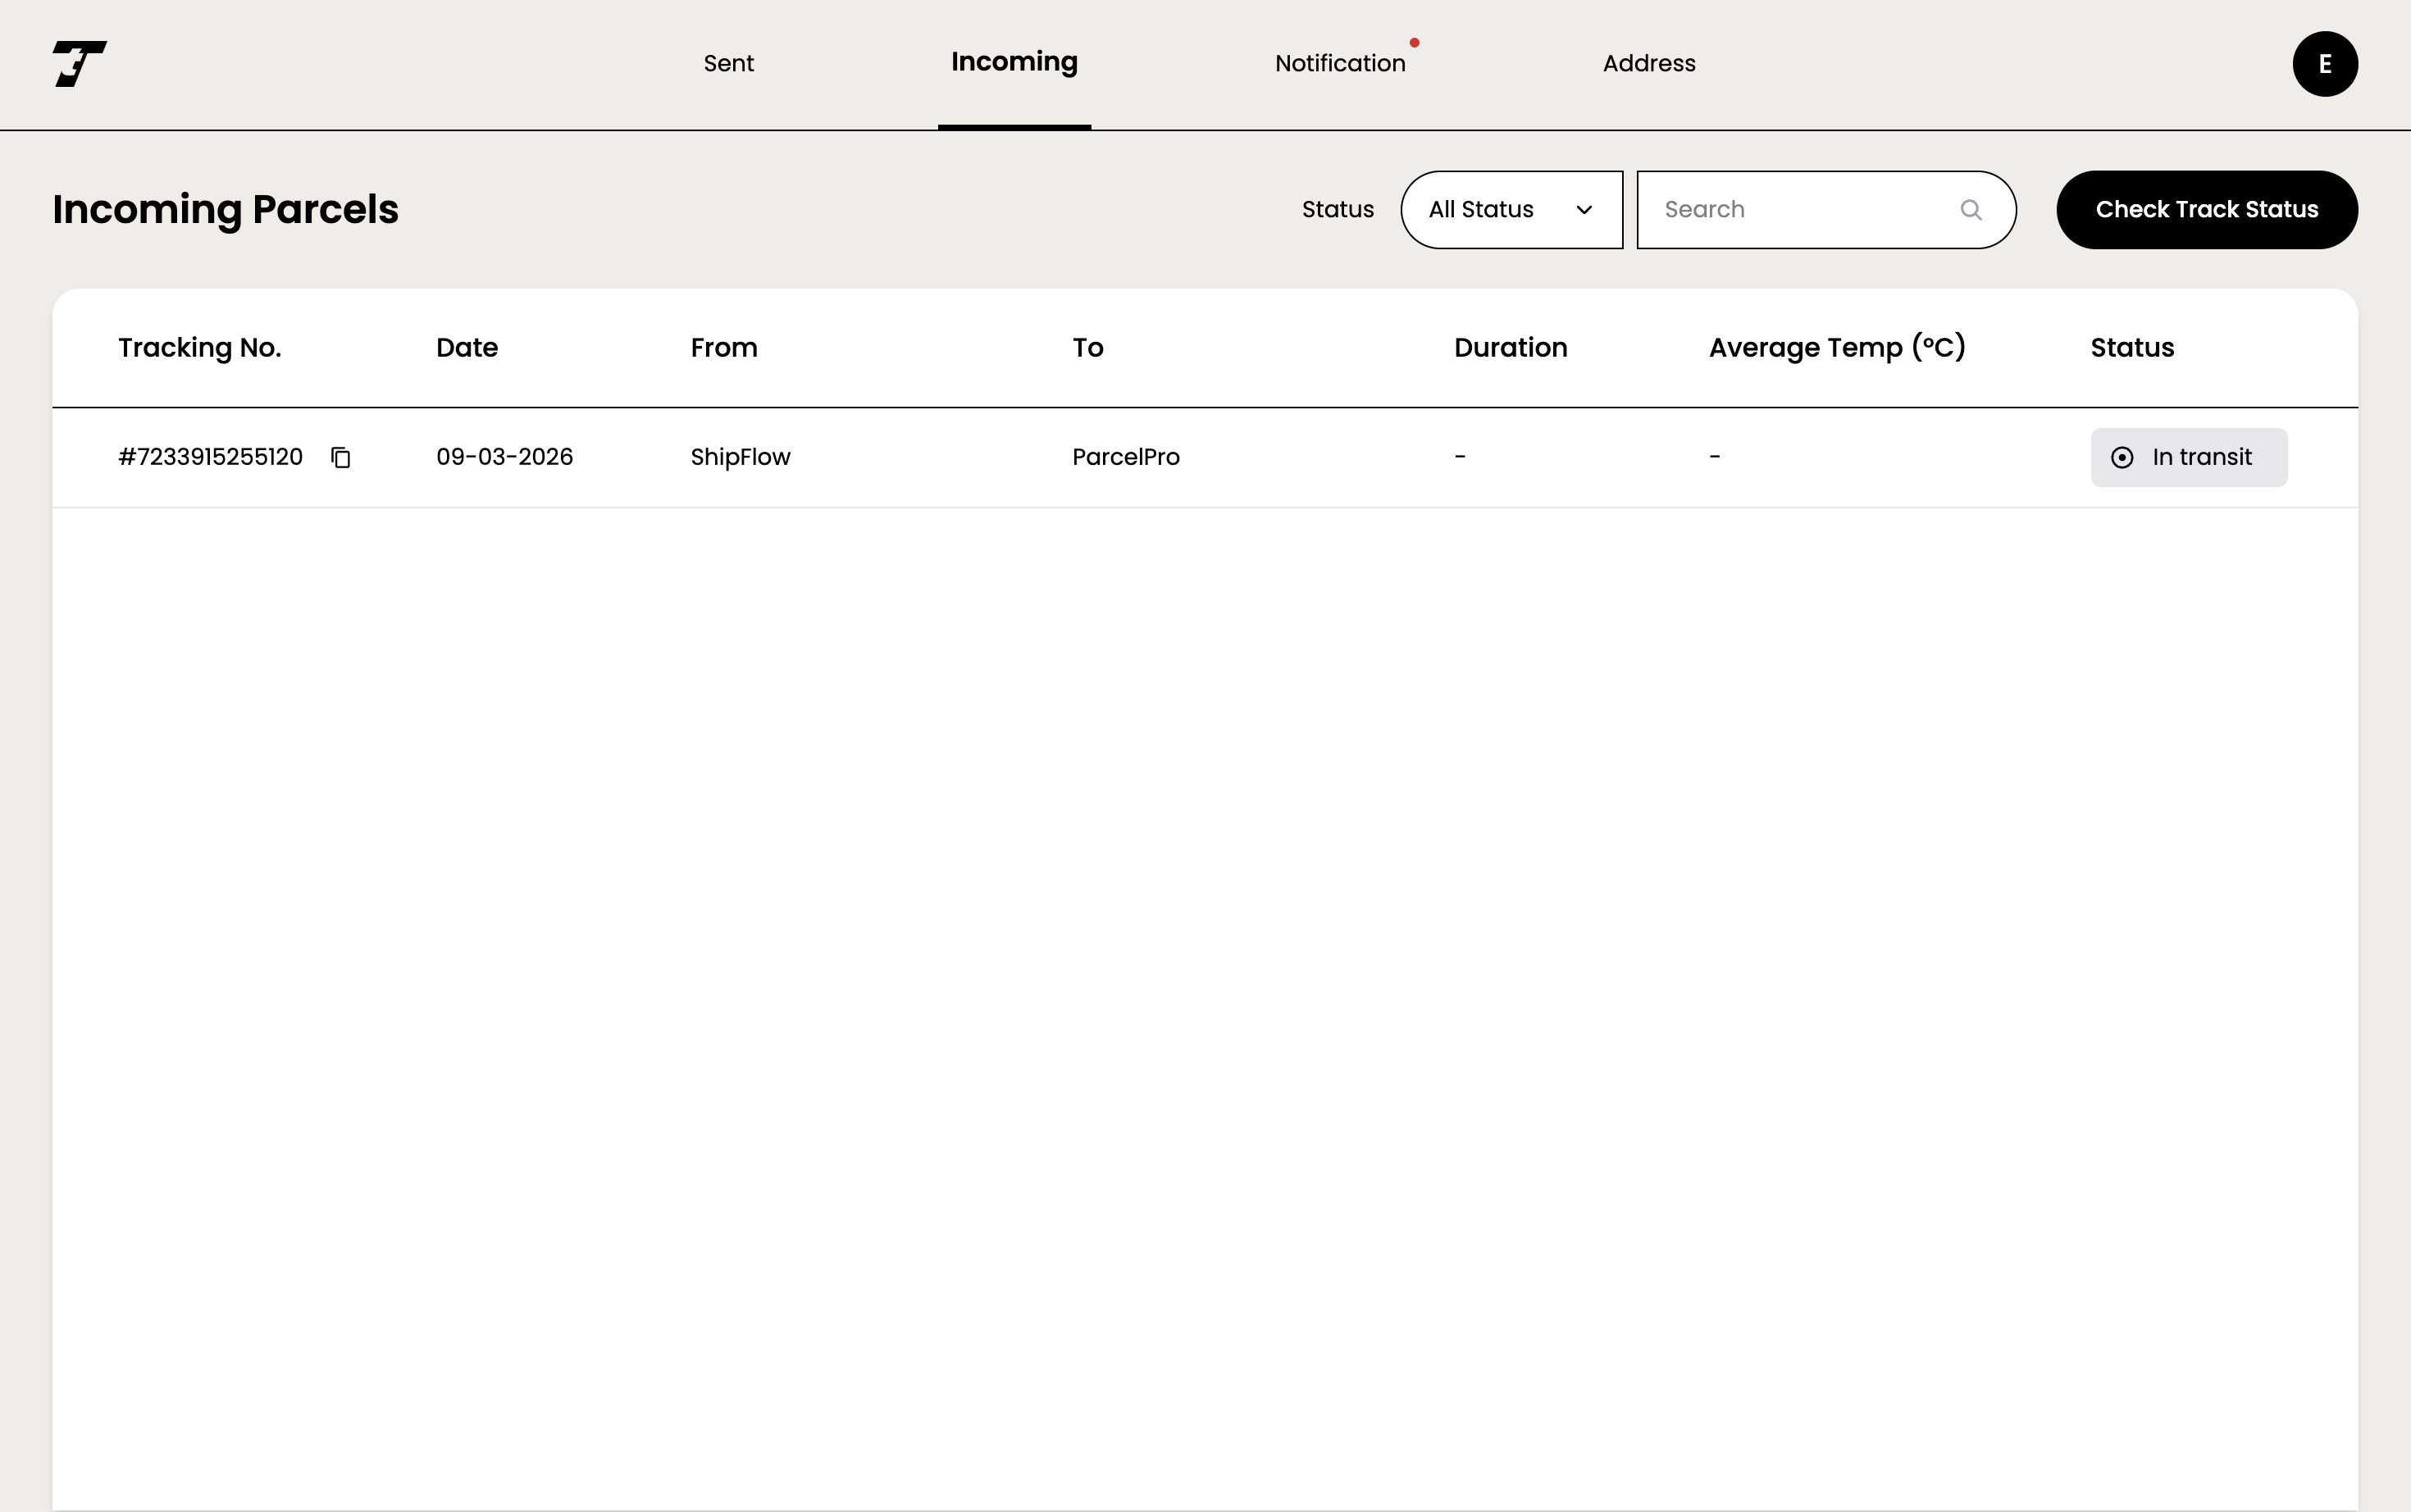
\includegraphics[width=0.8\textwidth]{incoming.png}
    \caption{หน้ากระดานสรุปผลรายการที่กำลังจัดส่ง}
    \label{fig:ui_user_dashboard_incoming}
\end{figure}
\end{minipage}

\vspace{1em}
\begin{minipage}{\linewidth}
\noindent \textbf{8. หน้ากระดานสรุปผลรายการที่ส่งแล้ว} \\
สำหรับดูประวัติและภาพรวมของพัสดุที่ \textbf{ผู้ส่งพัสดุ} ได้ทำการจัดส่งเสร็จสิ้นแล้ว
\begin{figure}[H]
    \centering
    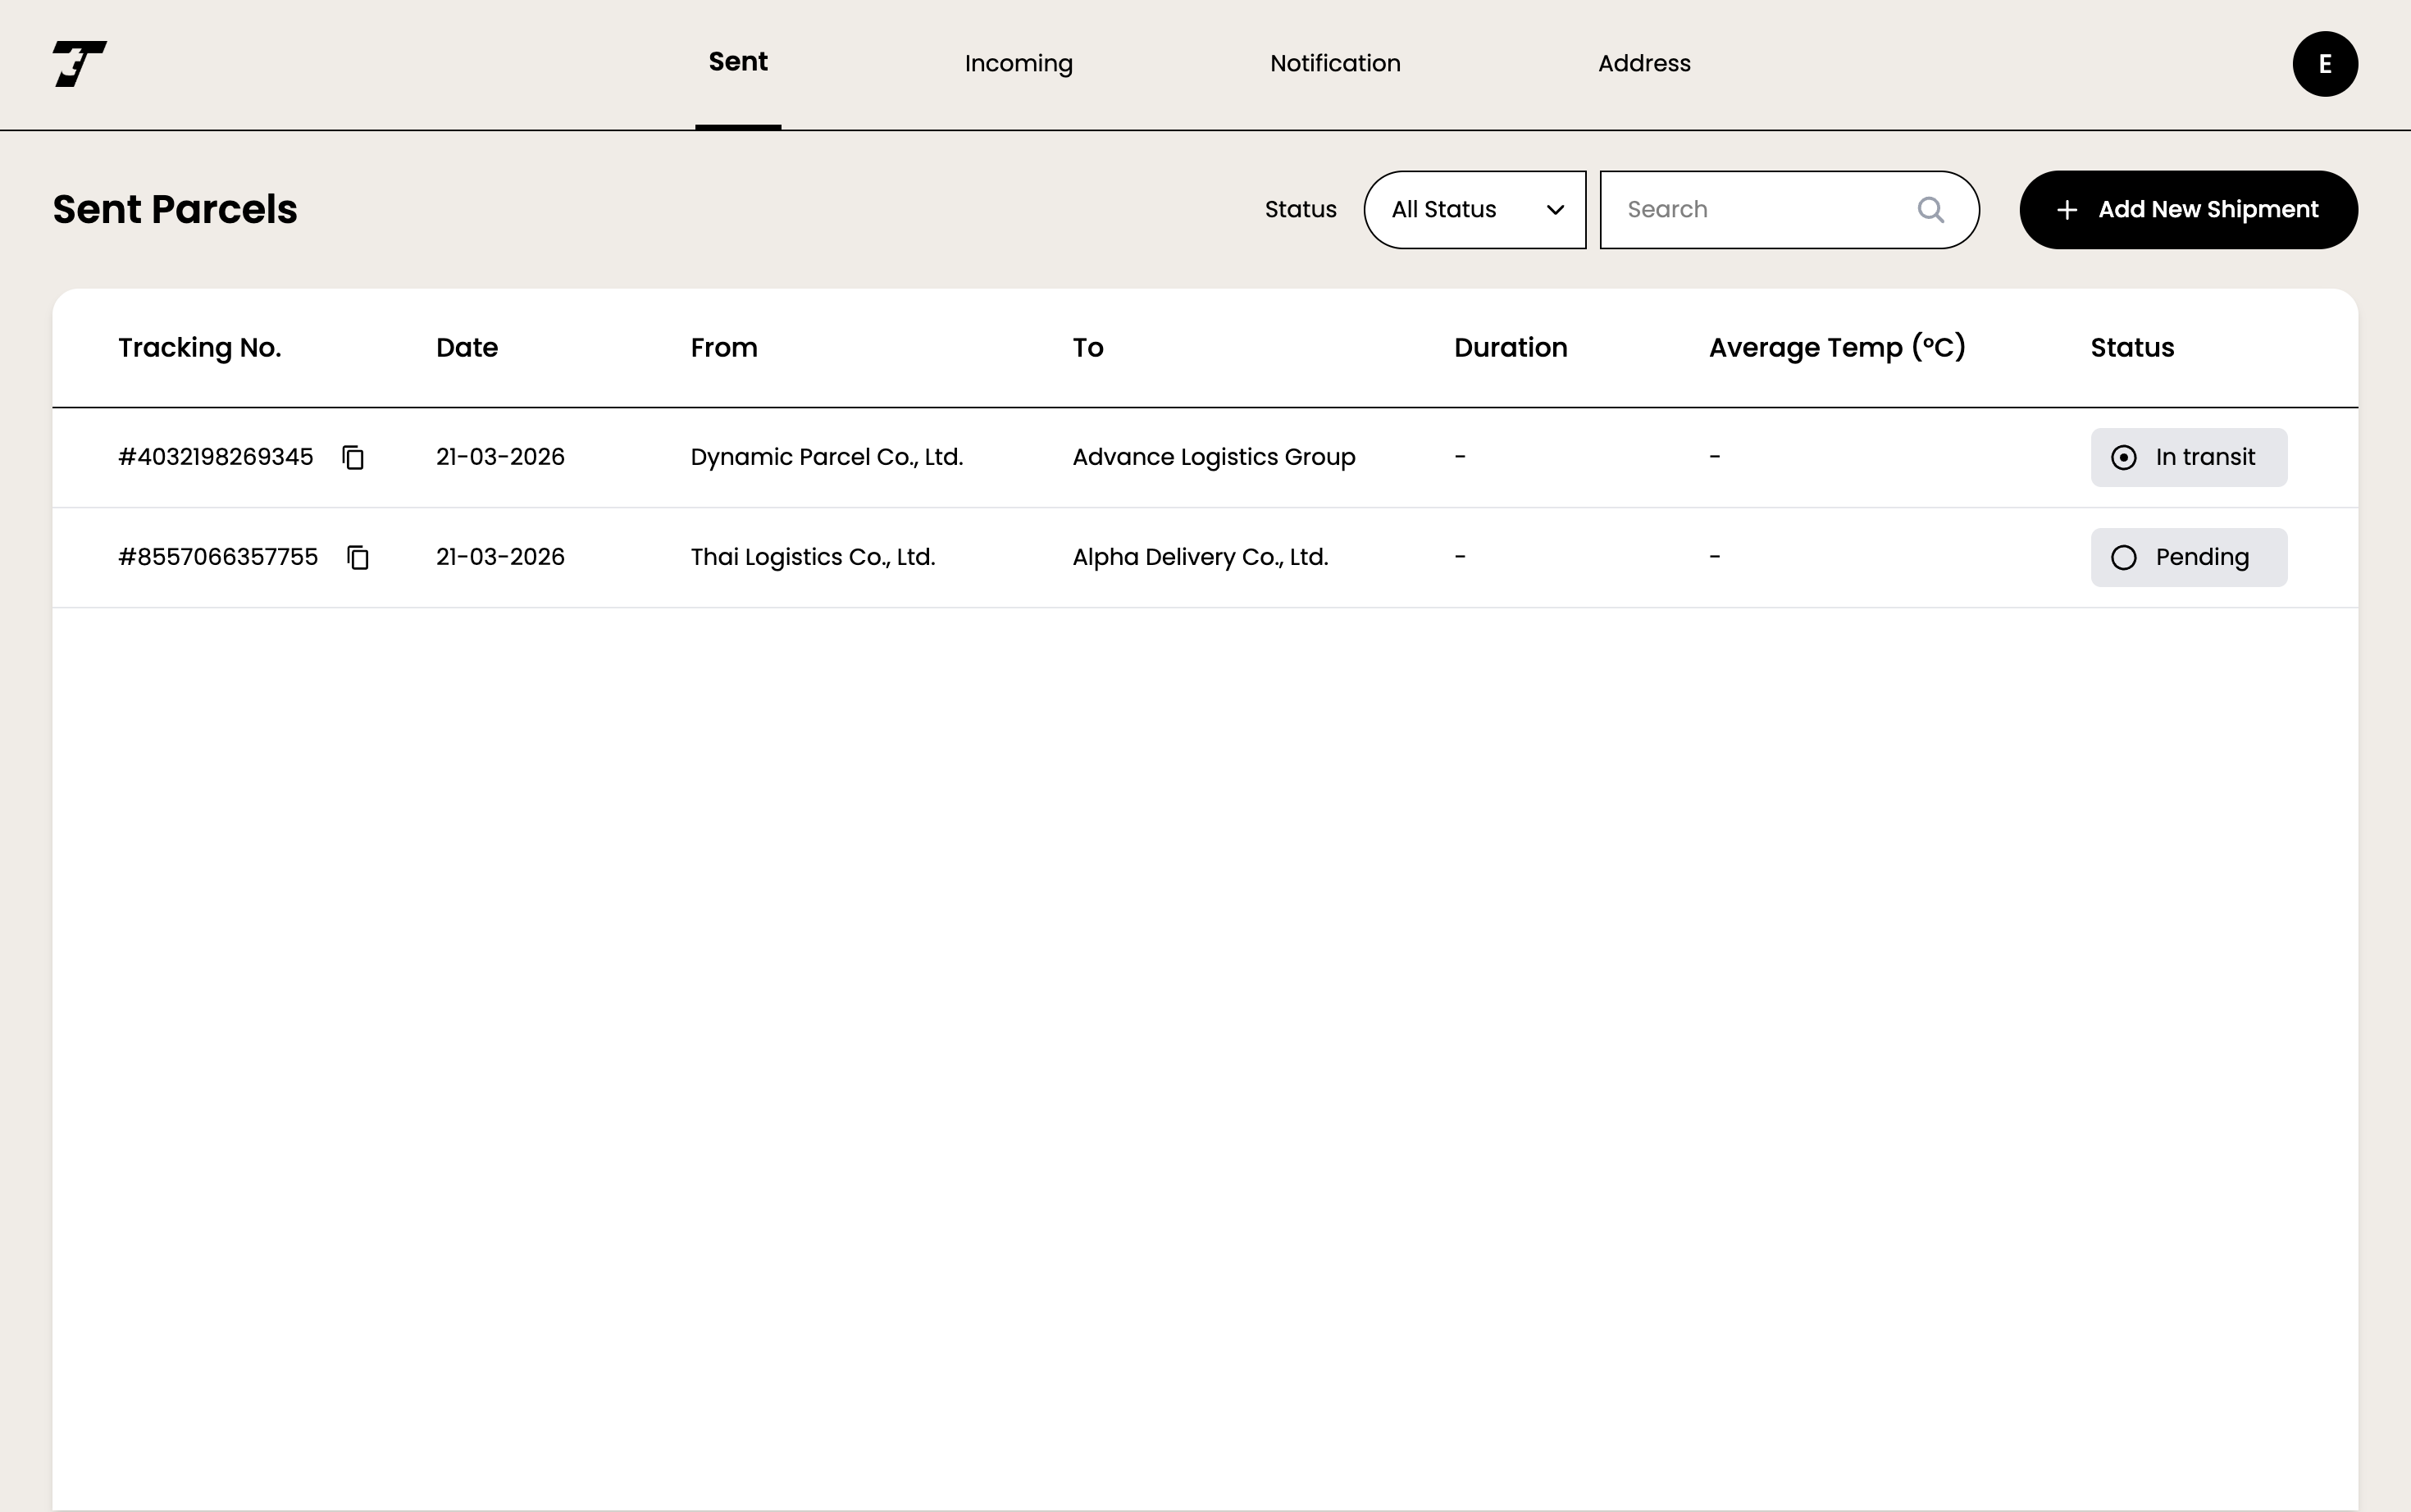
\includegraphics[width=0.8\textwidth]{sent.png}
    \caption{หน้ากระดานสรุปผลรายการที่ส่งแล้ว}
    \label{fig:ui_user_dashboard_sent}
\end{figure}
\end{minipage}

\vspace{1em}
\begin{minipage}{\linewidth}
\noindent \textbf{9. หน้าตรวจสอบอุณหภูมิแบบเรียลไทม์} \\
สำหรับให้ \textbf{ผู้ใช้งานทุกคนที่เกี่ยวข้อง} เฝ้าระวังและดูข้อมูลการเปลี่ยนแปลงของอุณหภูมิพัสดุ ณ เวลาปัจจุบัน (Real-time Monitoring)
\begin{figure}[H]
    \centering
    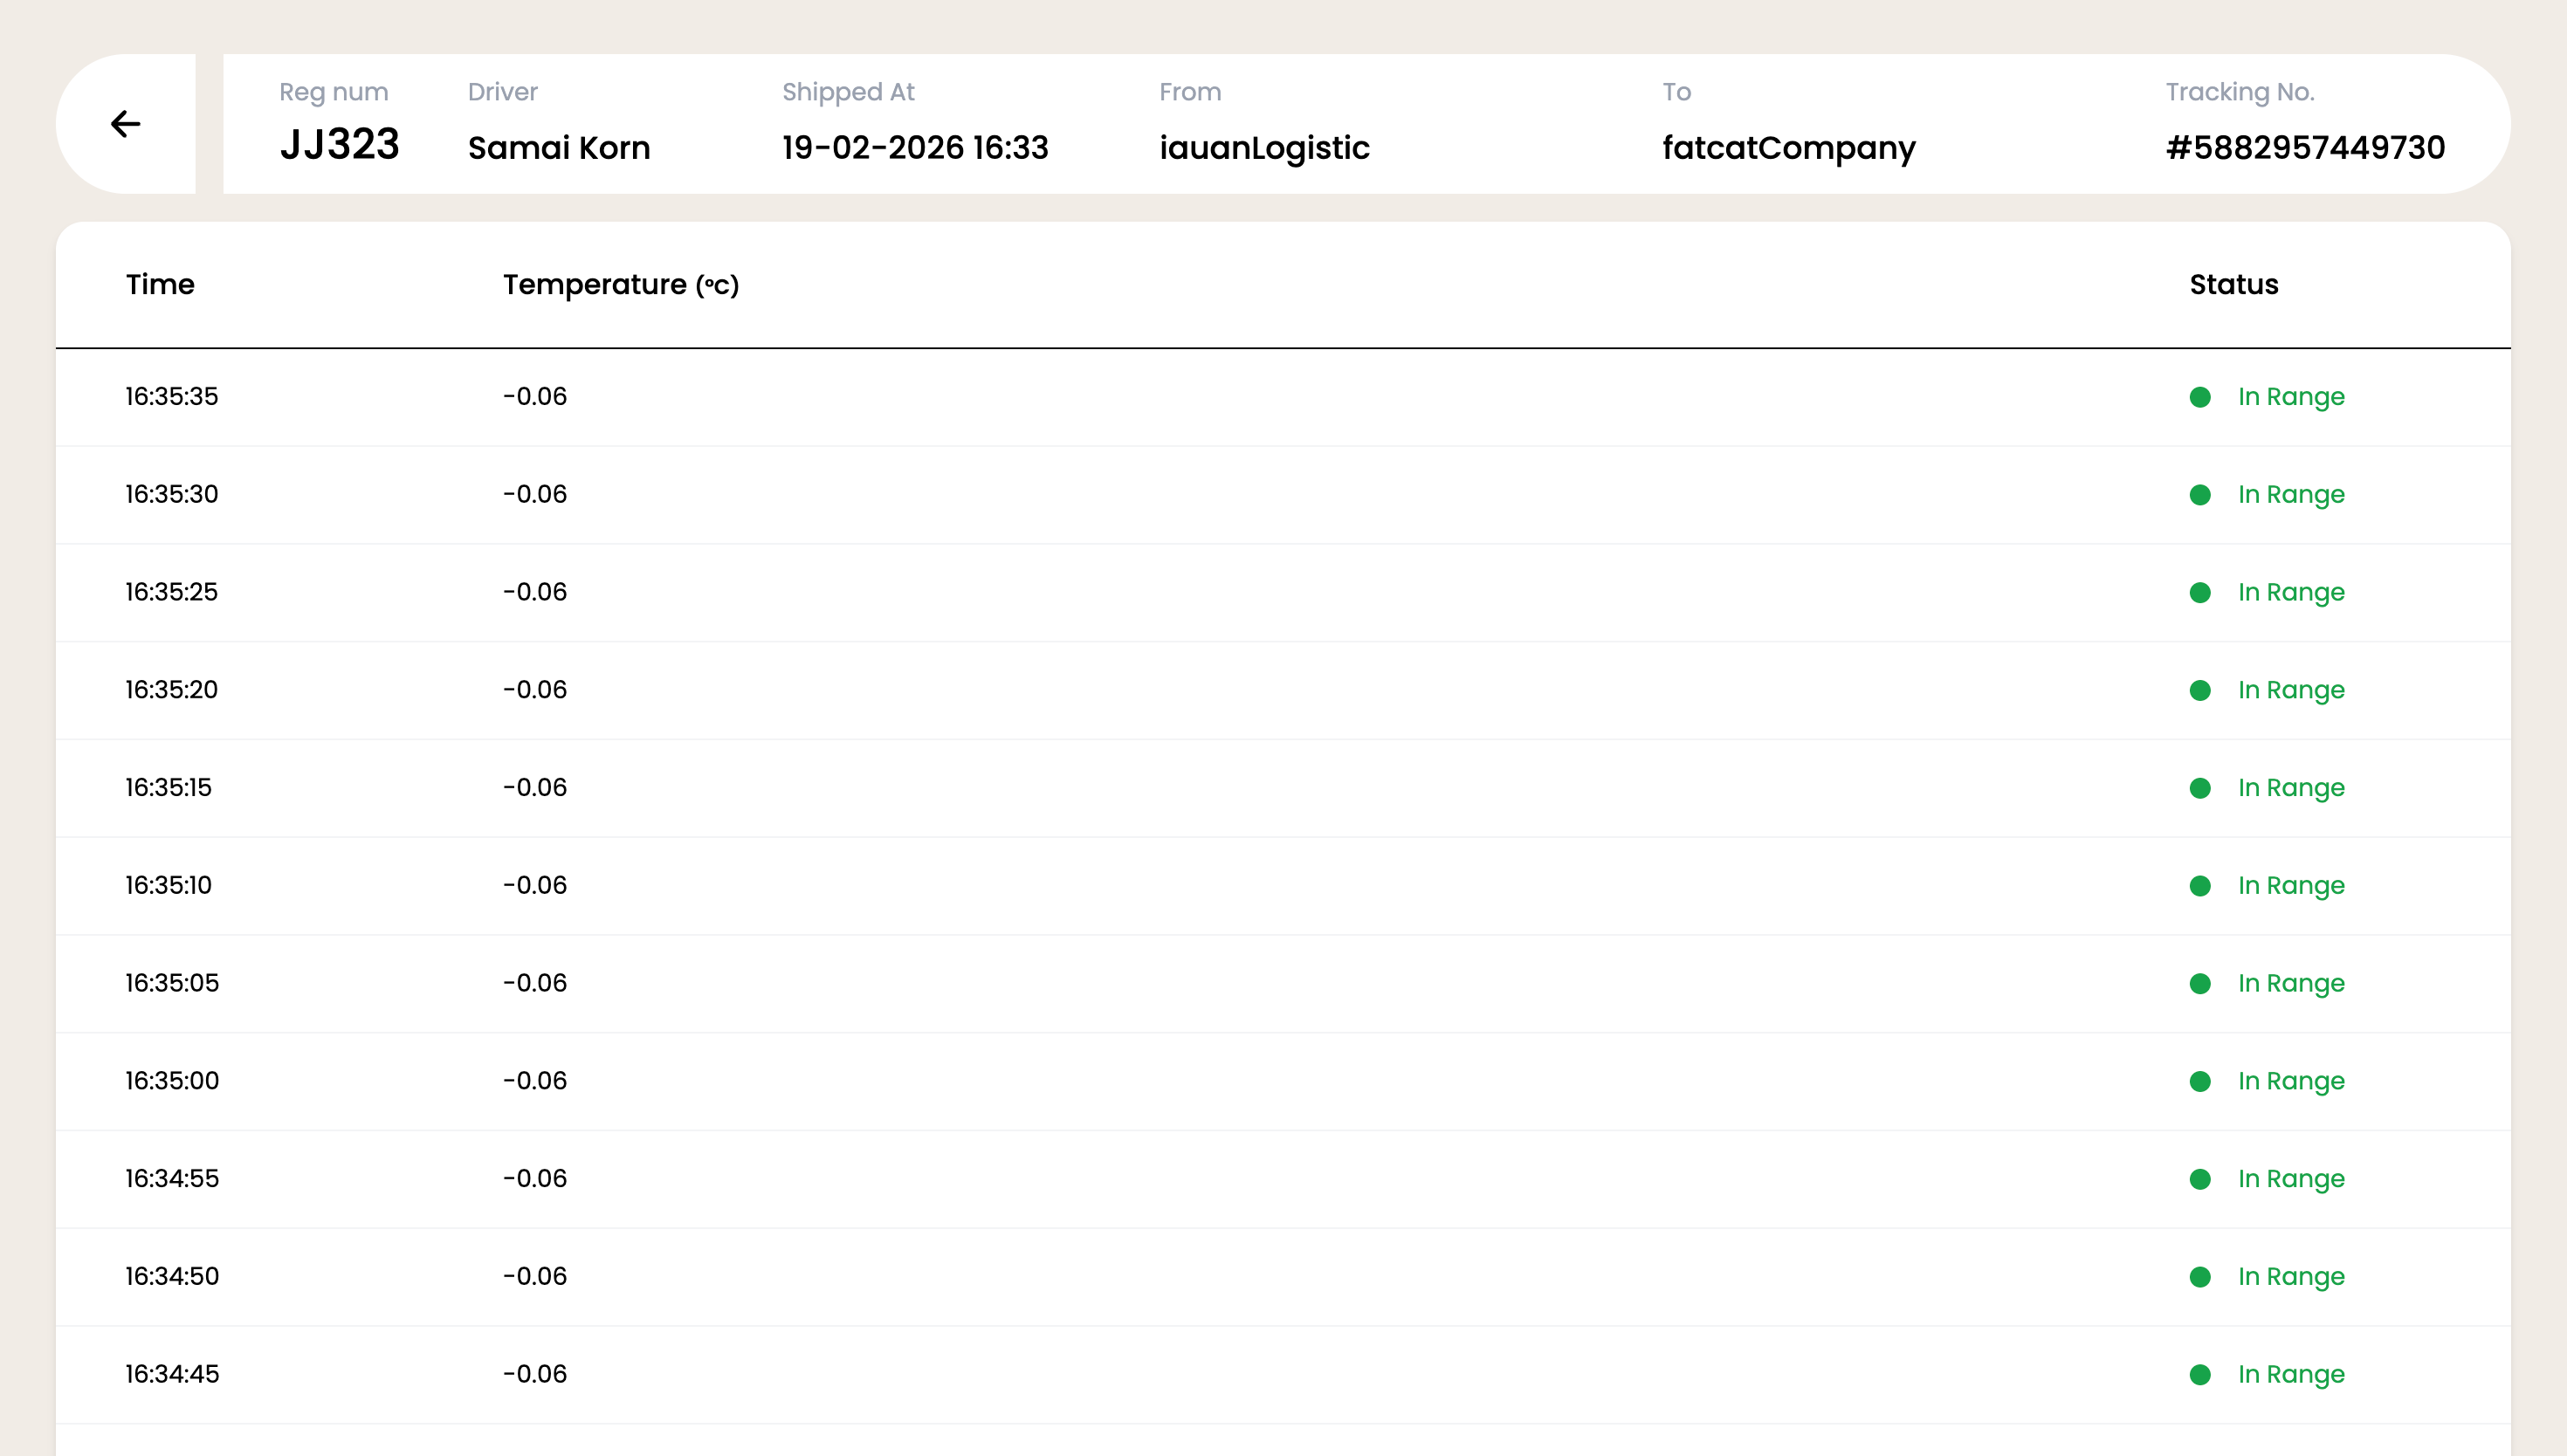
\includegraphics[width=0.8\textwidth]{log.png}
    \caption{หน้าตรวจสอบอุณหภูมิแบบเรียลไทม์}
    \label{fig:ui_user_log}
\end{figure}
\end{minipage}

\vspace{1em}
\begin{minipage}{\linewidth}
\noindent \textbf{10. หน้าการแจ้งเตือน} \\
แสดงการแจ้งเตือนสถานะความคืบหน้าของการจัดส่ง รวมถึงระบบแจ้งเตือนฉุกเฉินหากอุณหภูมิของสินค้าออกนอกเกณฑ์
\begin{figure}[H]
    \centering
    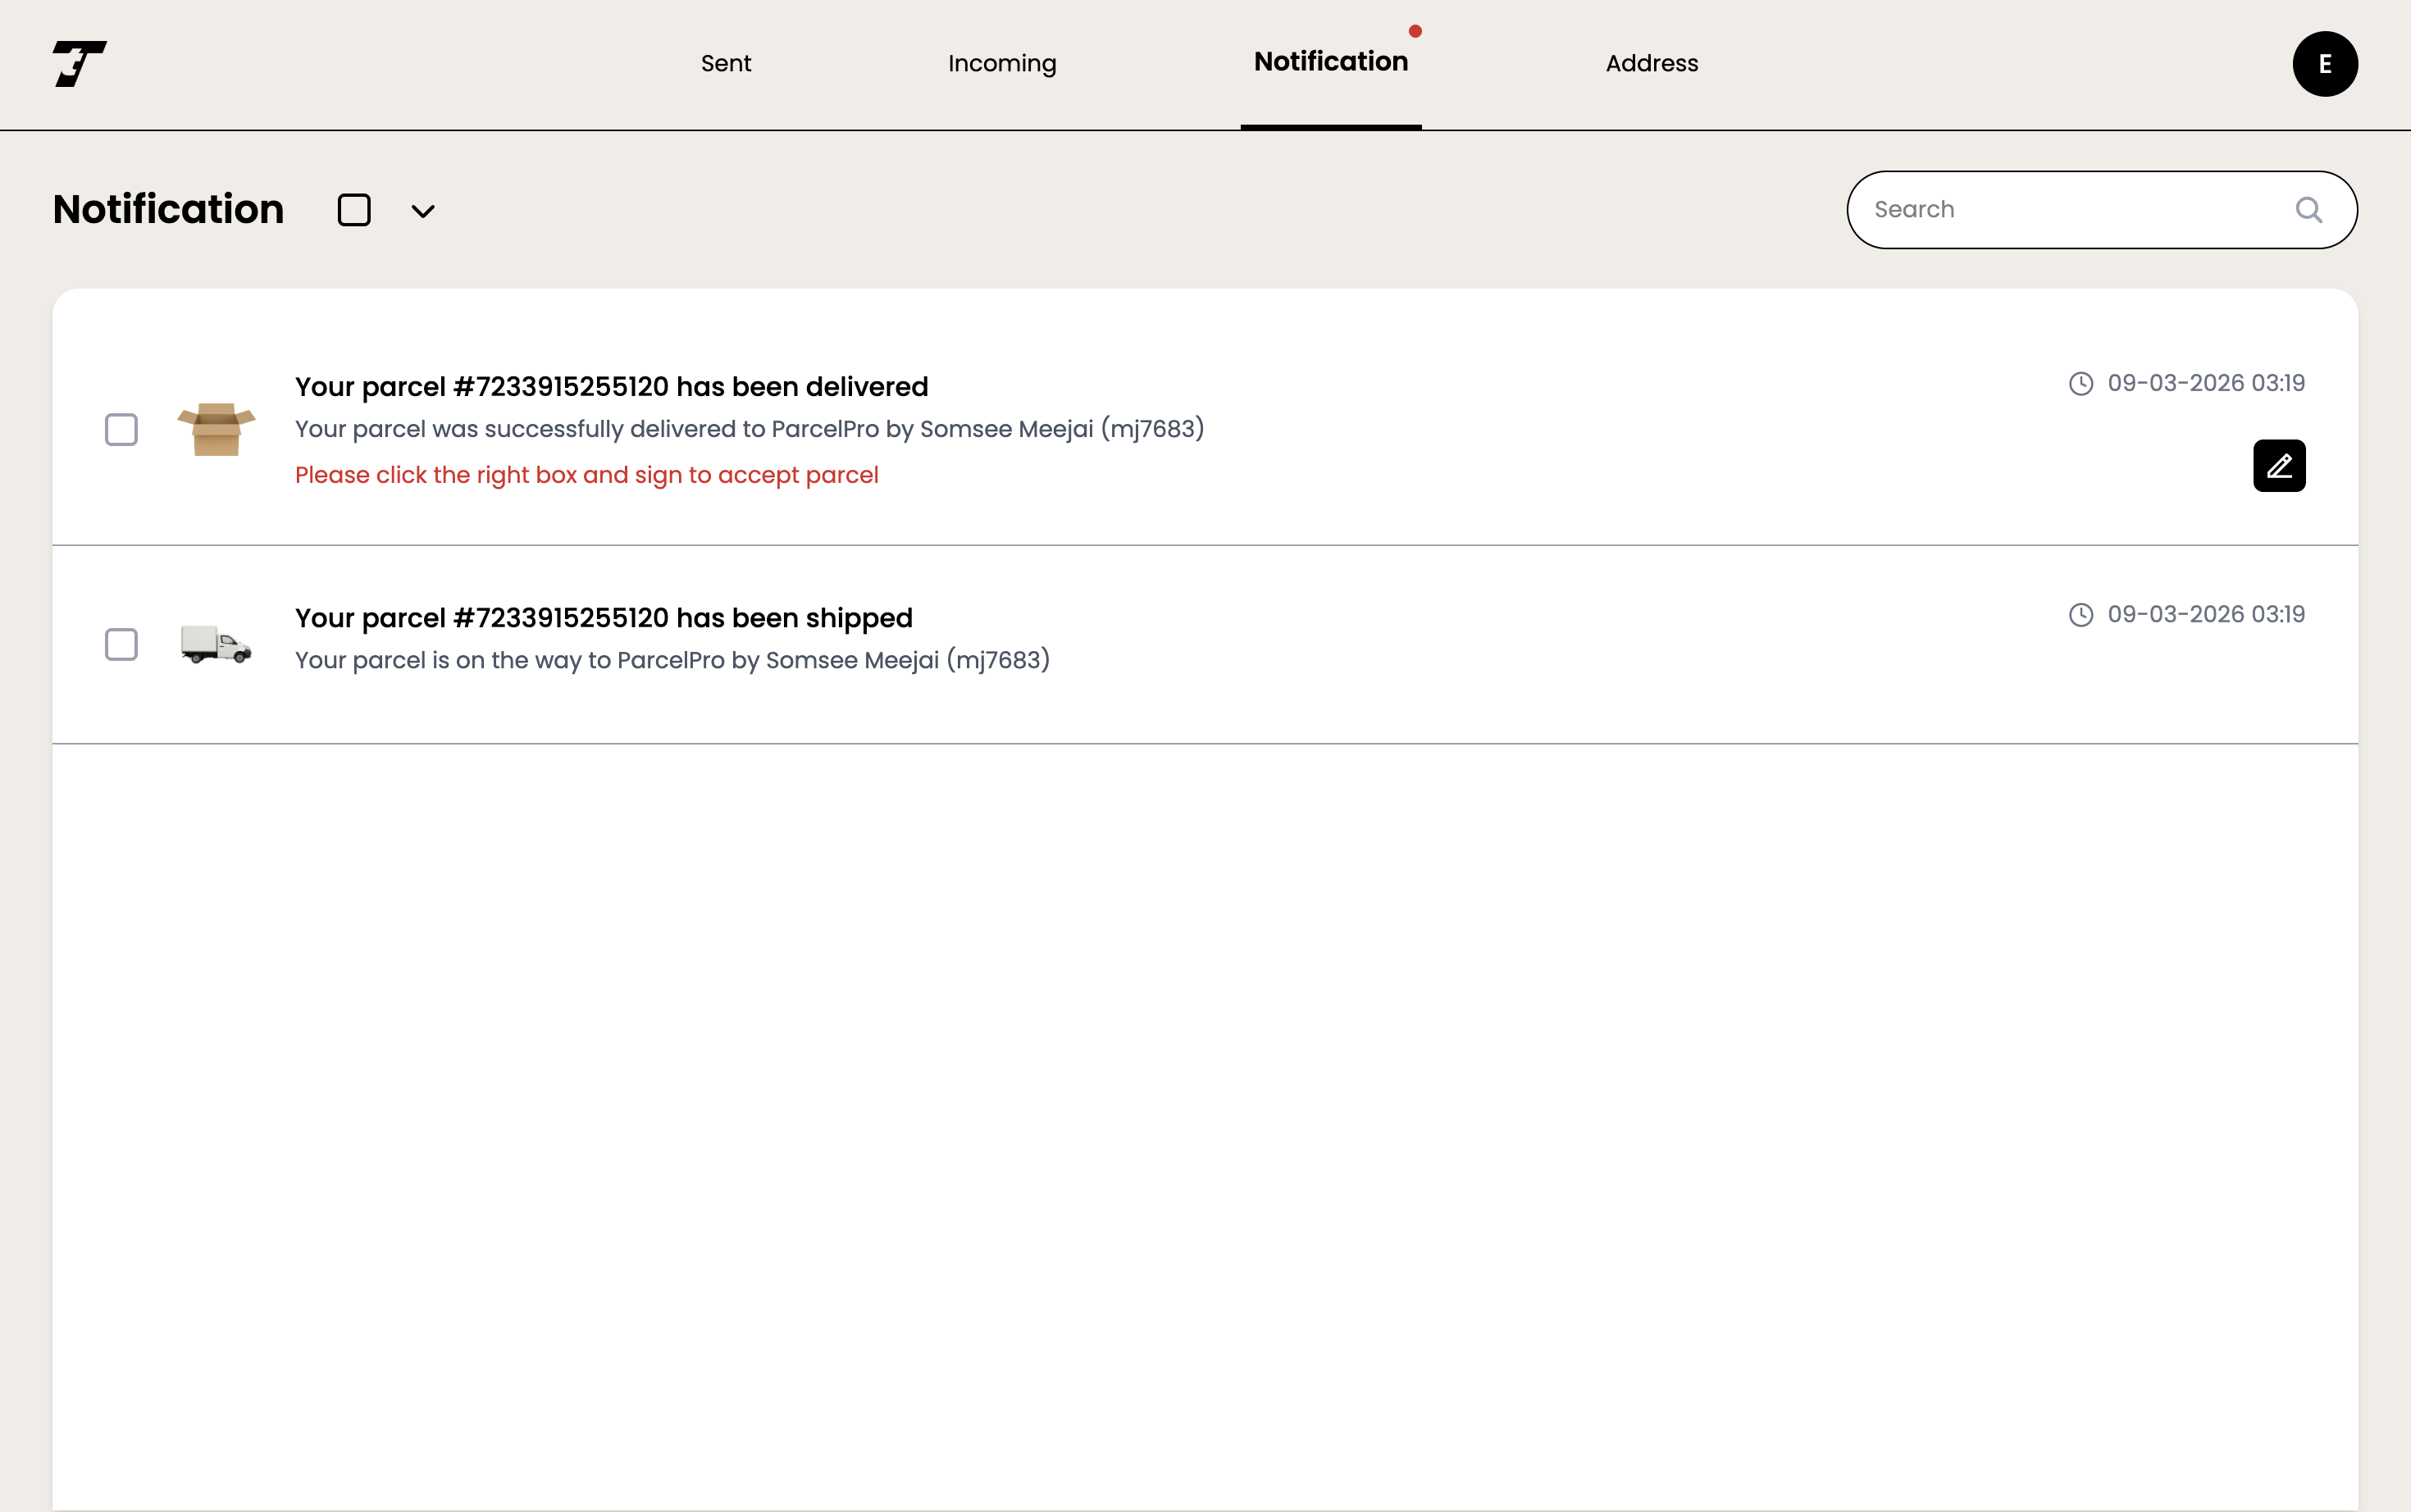
\includegraphics[width=0.8\textwidth]{notification.png}
    \caption{หน้าการแจ้งเตือนสำหรับผู้ใช้งานทั่วไป}
    \label{fig:ui_user_noti}
\end{figure}
\end{minipage}

\vspace{1em}
\begin{minipage}{\linewidth}
\noindent \textbf{11. หน้าลายมือชื่อดิจิทัล} \\
สำหรับให้ \textbf{ผู้รับพัสดุ} ทำการเซ็นชื่ออิเล็กทรอนิกส์ผ่านหน้าจอเพื่อยืนยันการรับสินค้าเมื่อพัสดุถูกส่งถึงปลายทาง
\begin{figure}[H]
    \centering
    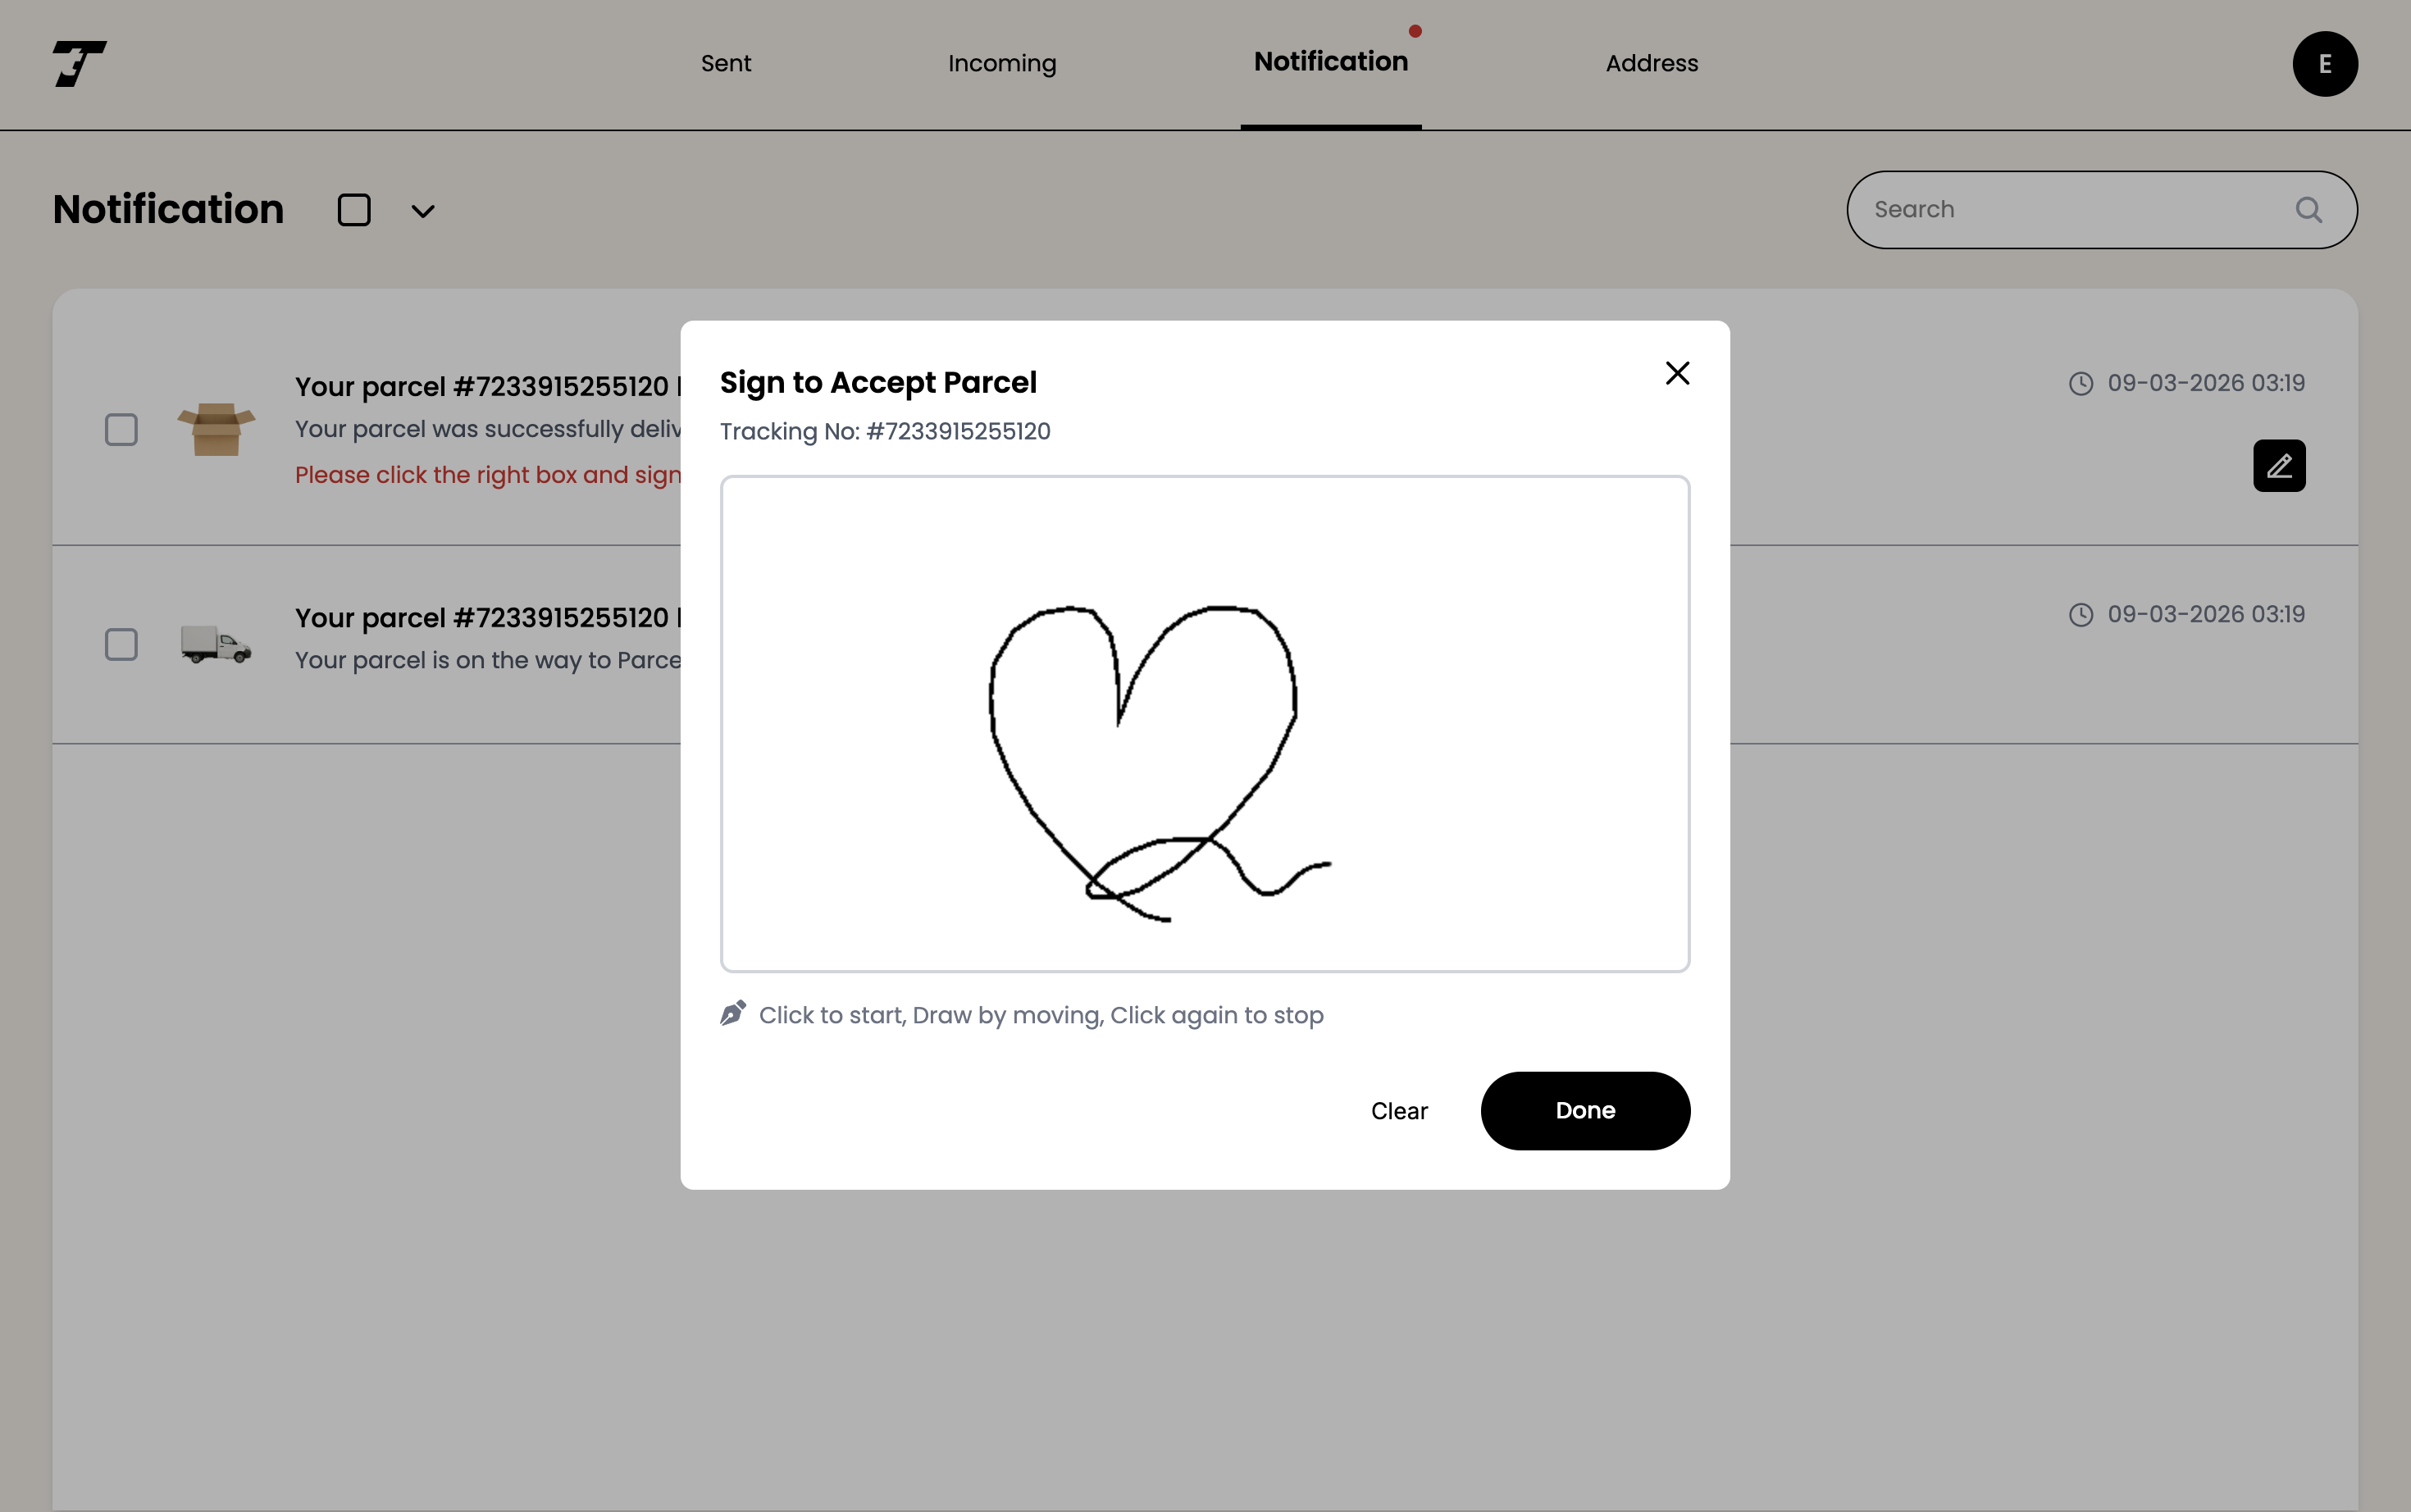
\includegraphics[width=0.8\textwidth]{digitalsignature.png}
    \caption{หน้าลายมือชื่อดิจิทัลสำหรับเซ็นรับพัสดุ}
    \label{fig:ui_user_signature}
\end{figure}
\end{minipage}

\vspace{1em}
\begin{minipage}{\linewidth}
\noindent \textbf{12. หน้าสรุปข้อมูลการขนส่ง} \\
หน้าต่างสรุปข้อมูลแบบเบ็ดเสร็จเมื่อการขนส่งเสร็จสิ้น โดยจะแสดงข้อมูลอุณหภูมิตั้งแต่เริ่มต้นจนถึงปลายทางในรูปแบบกราฟเชิงเวลา พร้อมทั้งแสดงสถานะการยืนยันความถูกต้องของข้อมูล (Verification) ผ่านบล็อกเชน
\begin{figure}[H]
    \centering
    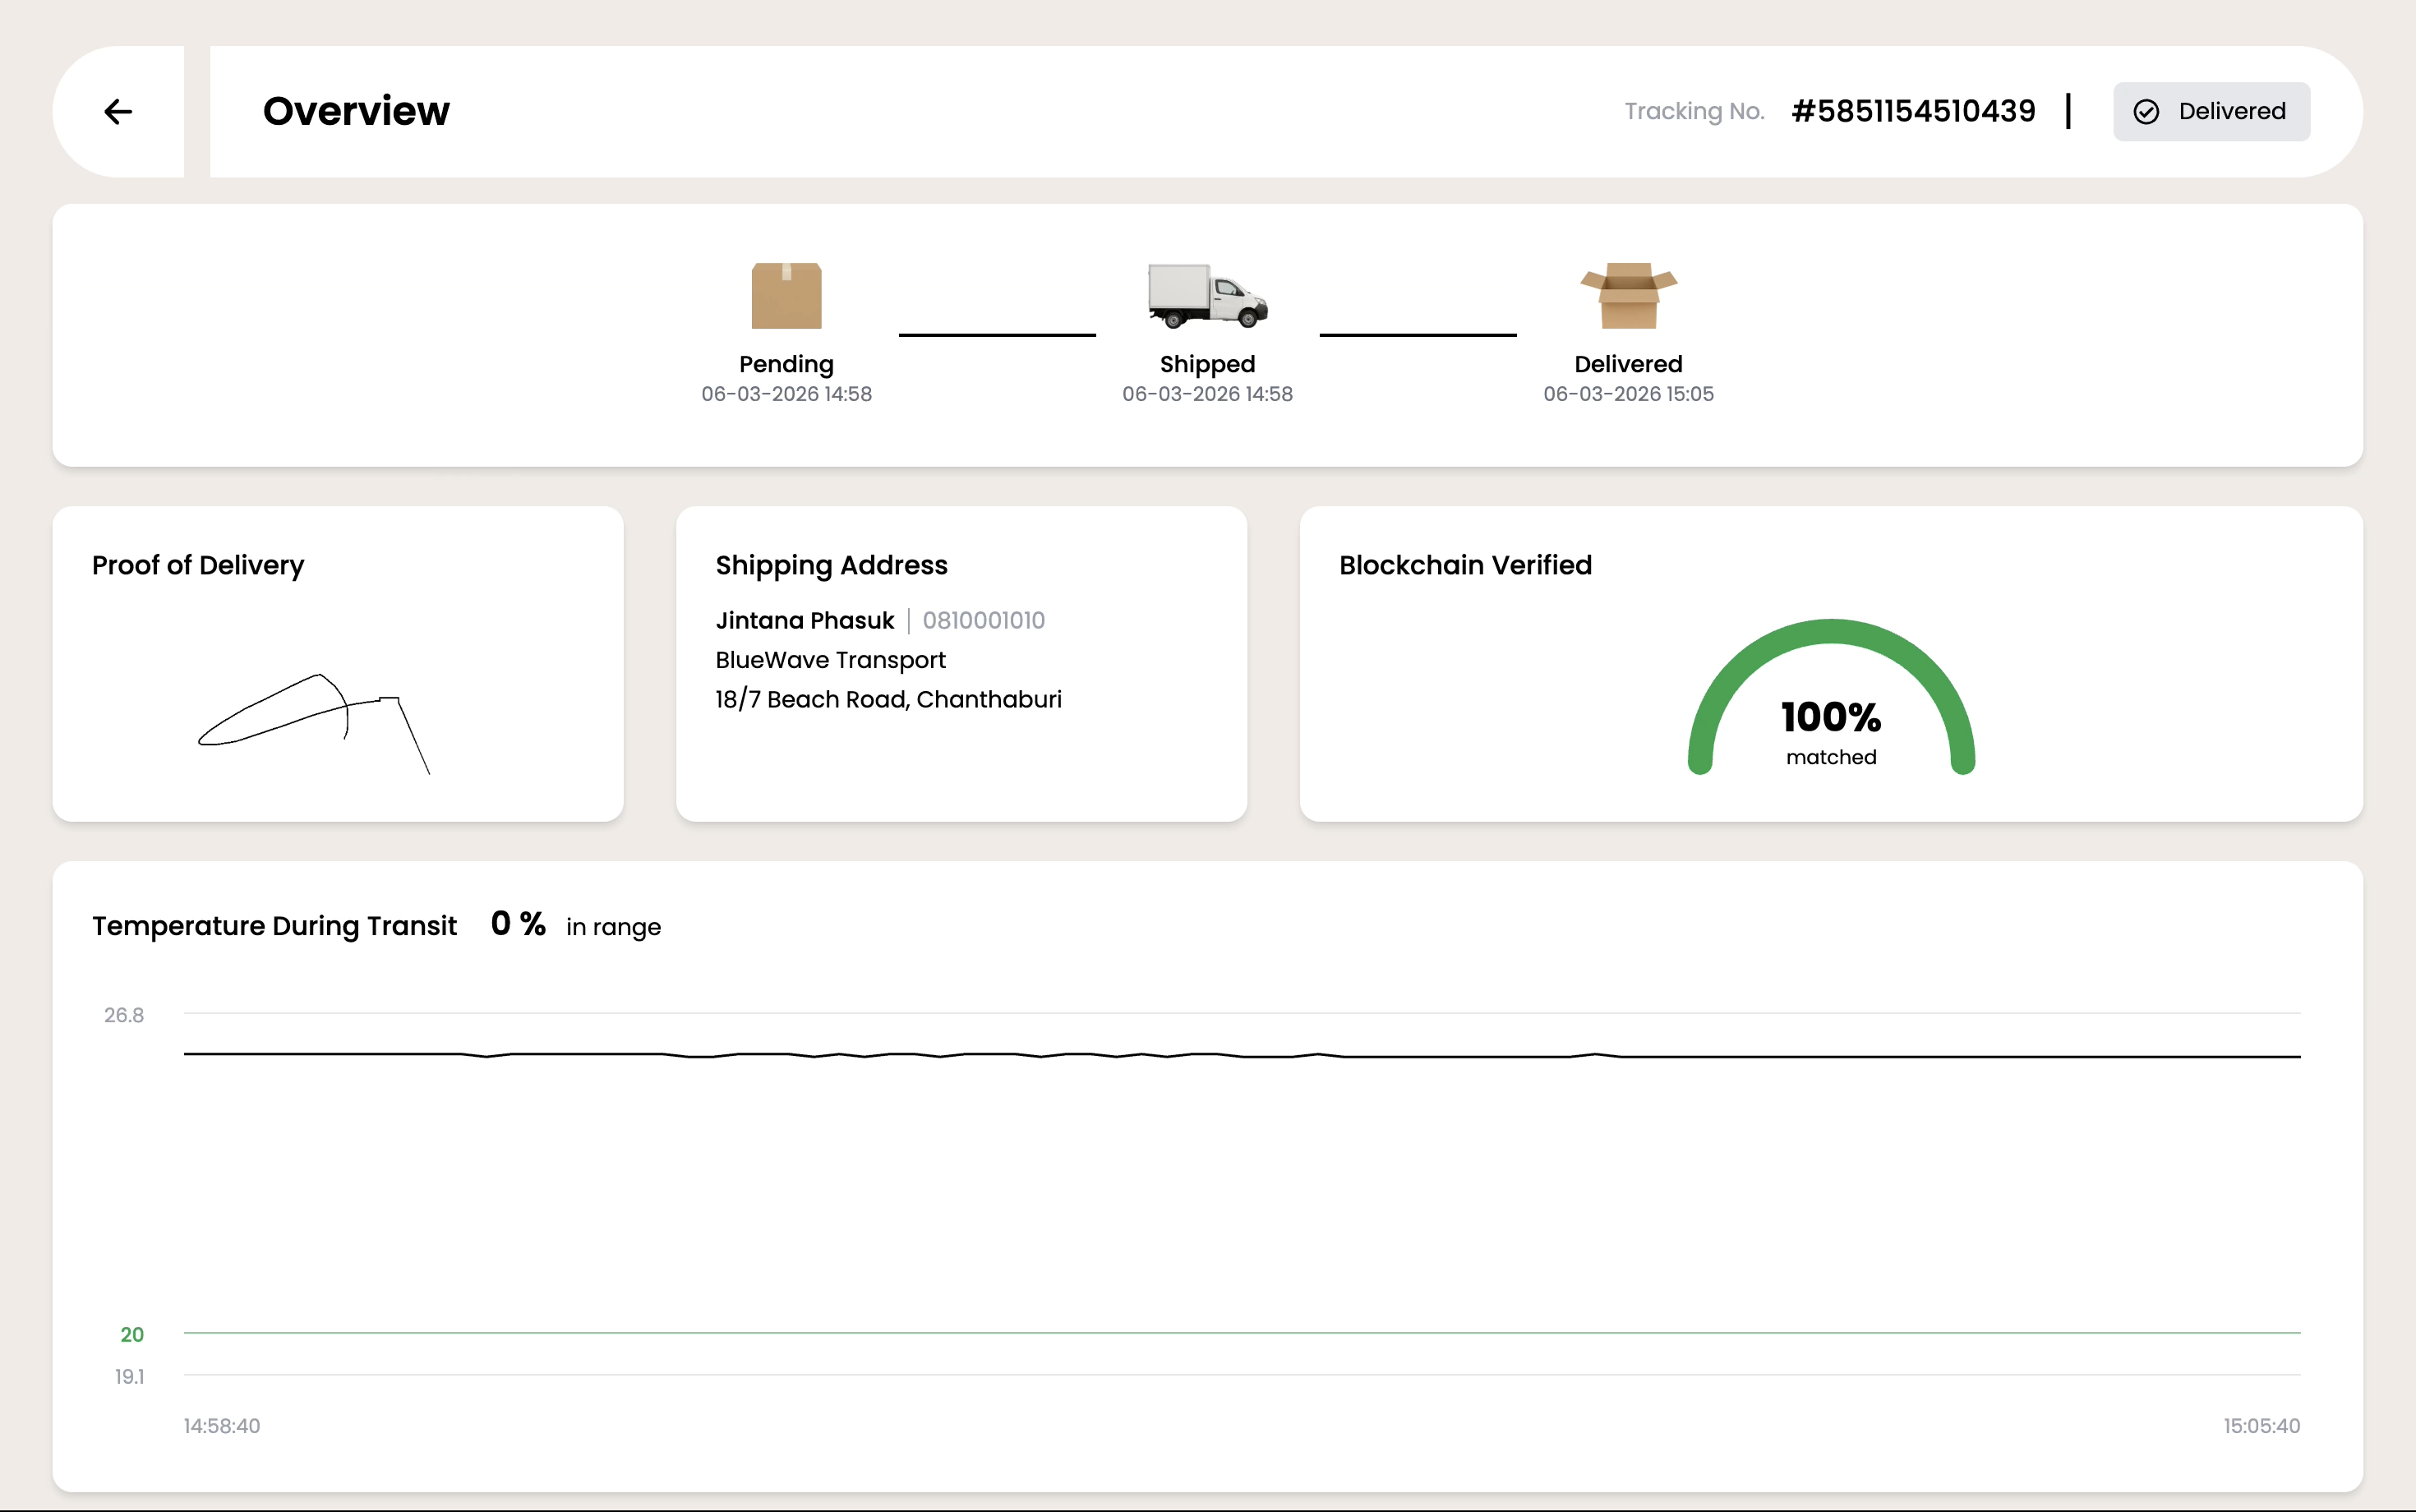
\includegraphics[width=0.8\textwidth]{overview.png}
    \caption{หน้าสรุปข้อมูลการขนส่งและการยืนยันความถูกต้องผ่านบล็อกเชน}
    \label{fig:ui_user_overview}
\end{figure}
\end{minipage}


\subsection{ส่วนของผู้ดูแลระบบ}
ส่วนนี้ถูกออกแบบมาสำหรับเจ้าหน้าที่ดูแลระบบเพื่อบริหารจัดการพนักงานขับรถและการจัดส่งพัสดุในภาพรวม ประกอบด้วยหน้าต่างการทำงานดังนี้:

\vspace{1em}
\begin{minipage}{\linewidth}
\noindent \textbf{1. หน้าเพิ่มข้อมูลคนขับรถ} \\
สำหรับเพิ่มรายชื่อและรายละเอียดของคนขับรถคนใหม่เข้าสู่ระบบ เพื่อเตรียมความพร้อมในการจัดส่งพัสดุ
\begin{figure}[H]
    \centering
    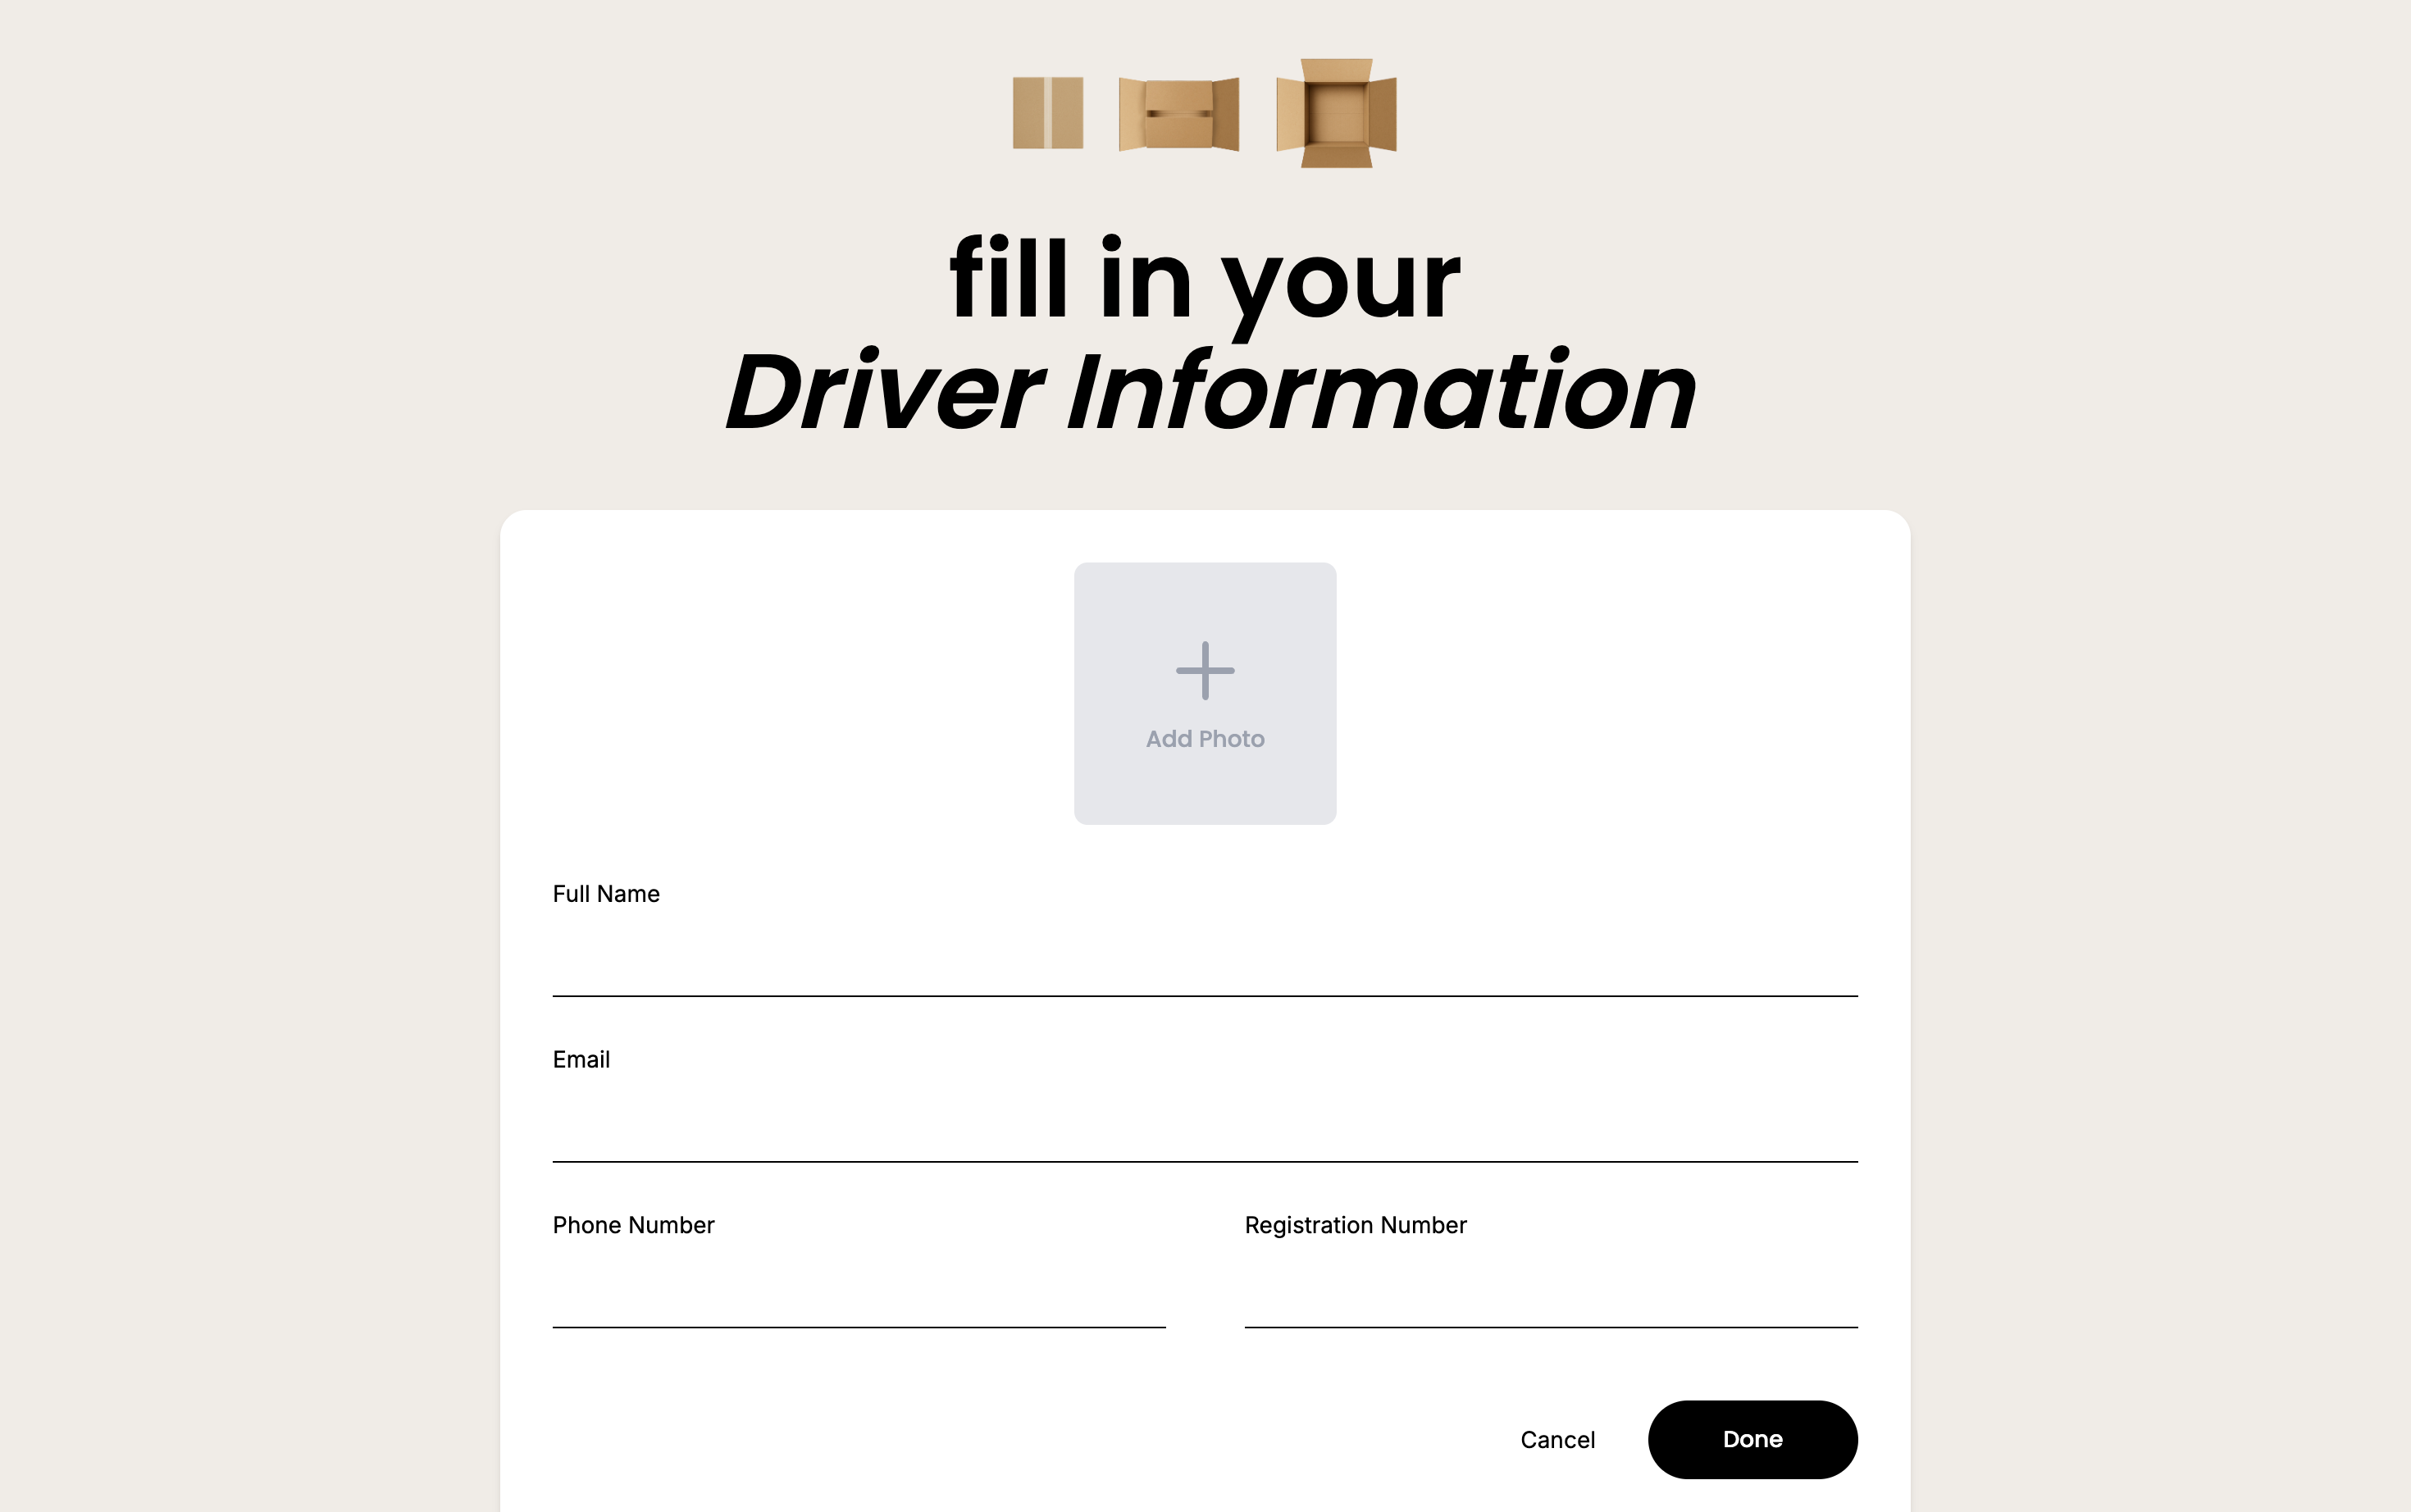
\includegraphics[width=0.8\textwidth]{admin_add_driver.png}
    \caption{หน้าเพิ่มข้อมูลคนขับรถ}
    \label{fig:ui_admin_add_driver}
\end{figure}
\end{minipage}

\vspace{1em}
\begin{minipage}{\linewidth}
\noindent \textbf{2. หน้าแสดงข้อมูลคนขับและพัสดุที่กำลังจัดส่ง} \\
สำหรับดูรายชื่อคนขับทั้งหมด พร้อมทั้งตรวจสอบพัสดุที่แต่ละคนกำลังรับผิดชอบจัดส่งอยู่ในขณะนั้น
\begin{figure}[H]
    \centering
    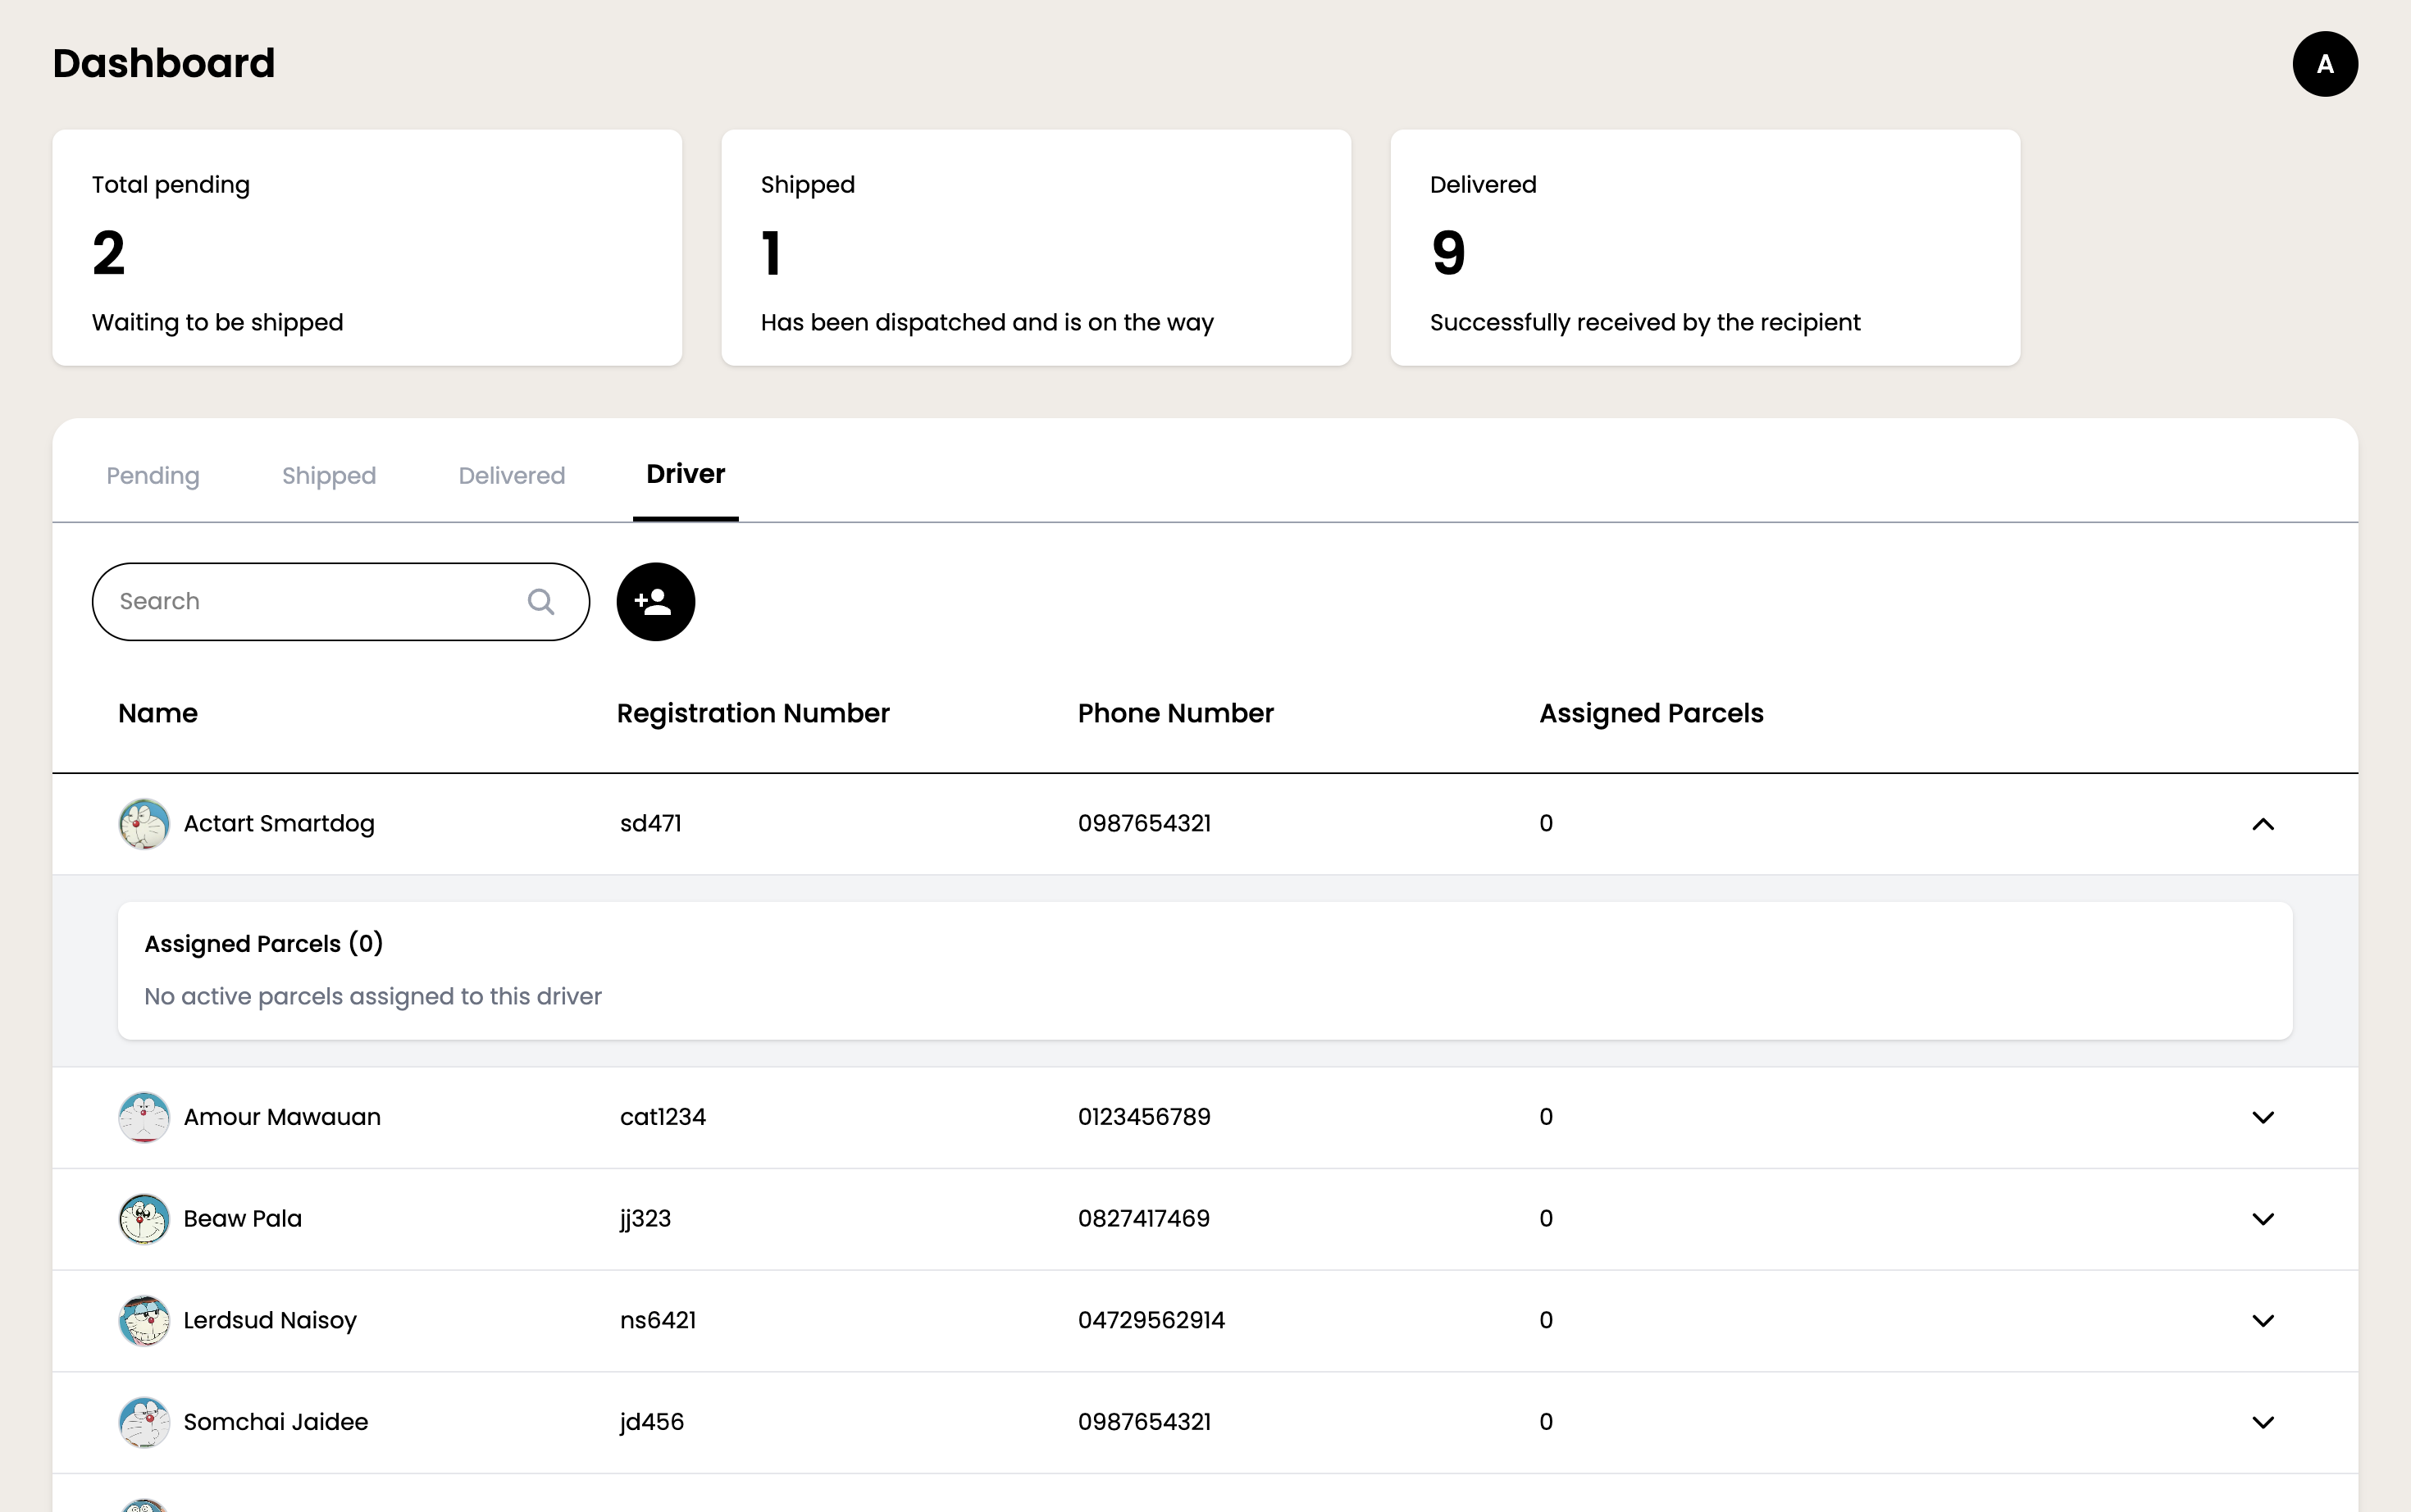
\includegraphics[width=0.8\textwidth]{admin_driver_list.png}
    \caption{หน้าแสดงข้อมูลคนขับและพัสดุที่กำลังจัดส่ง}
    \label{fig:ui_admin_driver_list}
\end{figure}
\end{minipage}

\vspace{1em}
\begin{minipage}{\linewidth}
\noindent \textbf{3. หน้าพัสดุที่รอการจัดสรรคนขับ} \\
สำหรับแสดงรายการพัสดุที่เข้าสู่ระบบ และกำลังรอให้ผู้ดูแลระบบเลือกคนขับรถที่เหมาะสมเพื่อเริ่มต้นการจัดส่ง
\begin{figure}[H]
    \centering
    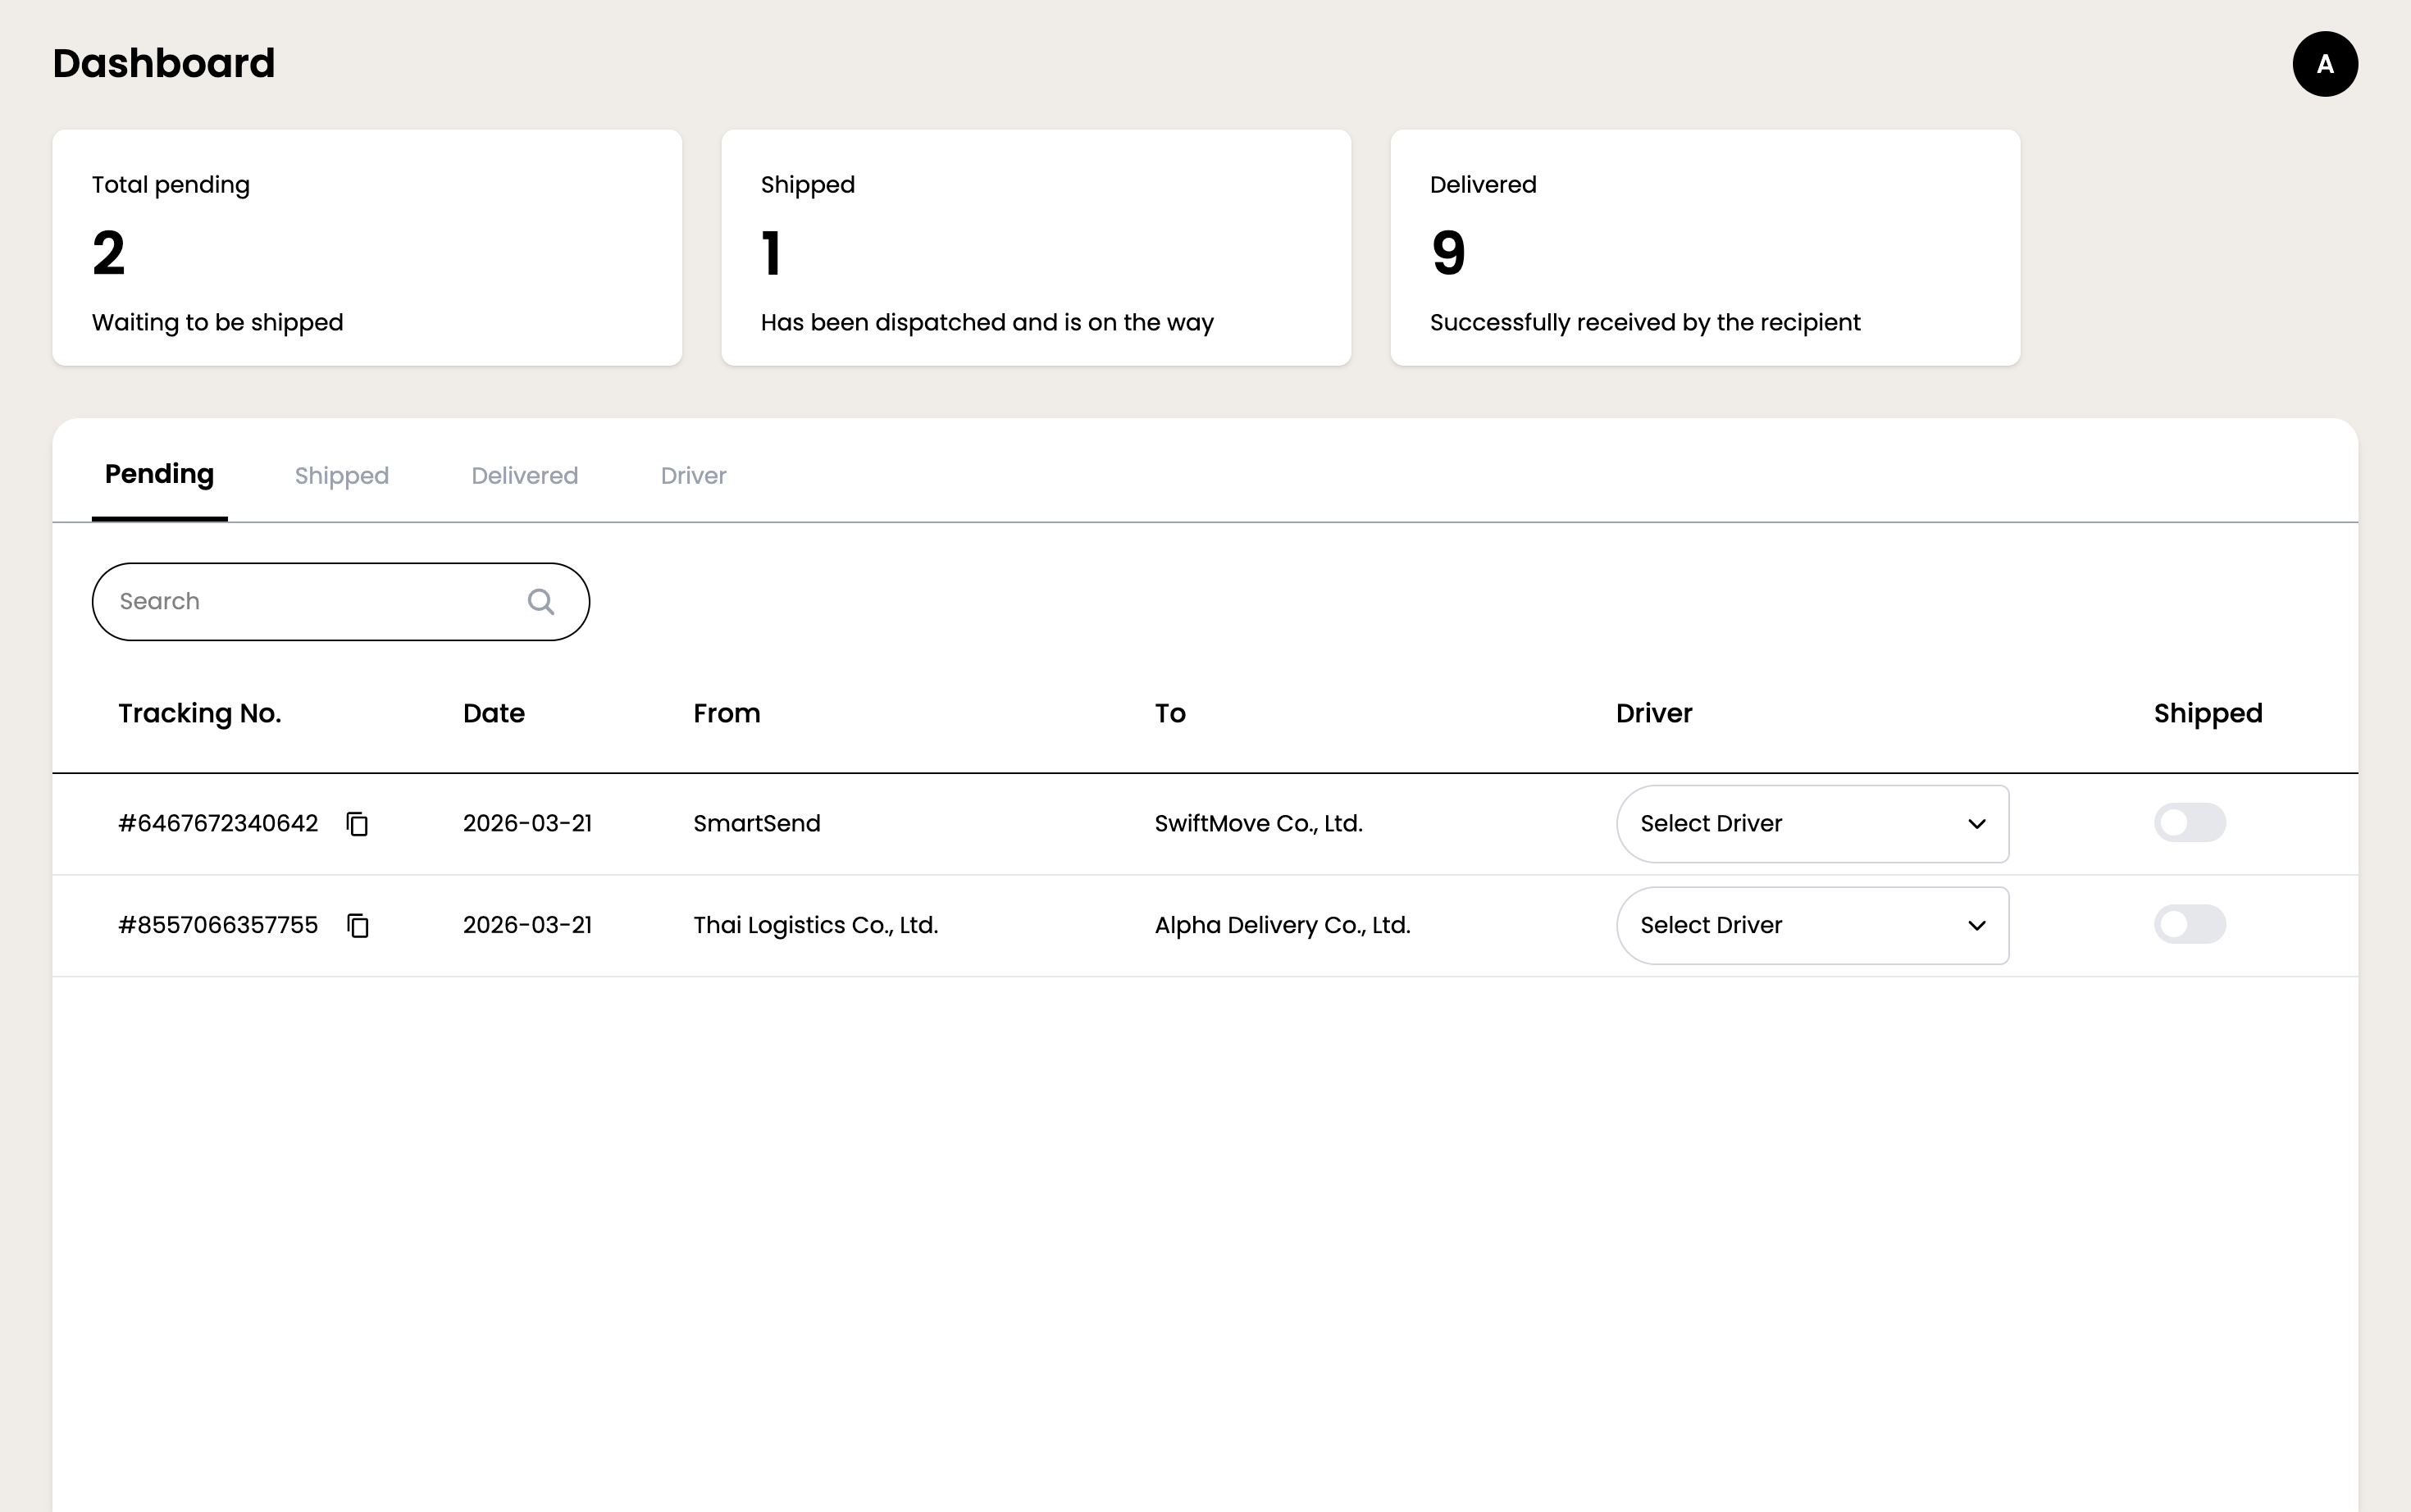
\includegraphics[width=0.8\textwidth]{admin_pending_parcels.png}
    \caption{หน้าพัสดุที่รอเลือกคนขับเพื่อเริ่มการจัดส่ง}
    \label{fig:ui_admin_pending_parcels}
\end{figure}
\end{minipage}

\vspace{1em}
\begin{minipage}{\linewidth}
\noindent \textbf{4. หน้าอัปเดตสถานะการจัดส่ง} \\
สำหรับให้ผู้ดูแลระบบเข้ามาปรับเปลี่ยนสถานะของพัสดุในระบบ เช่น เปลี่ยนจากสถานะอยู่ระหว่างการจัดส่ง (Shipped) เป็นจัดส่งสำเร็จแล้ว (Delivered)
\begin{figure}[H]
    \centering
    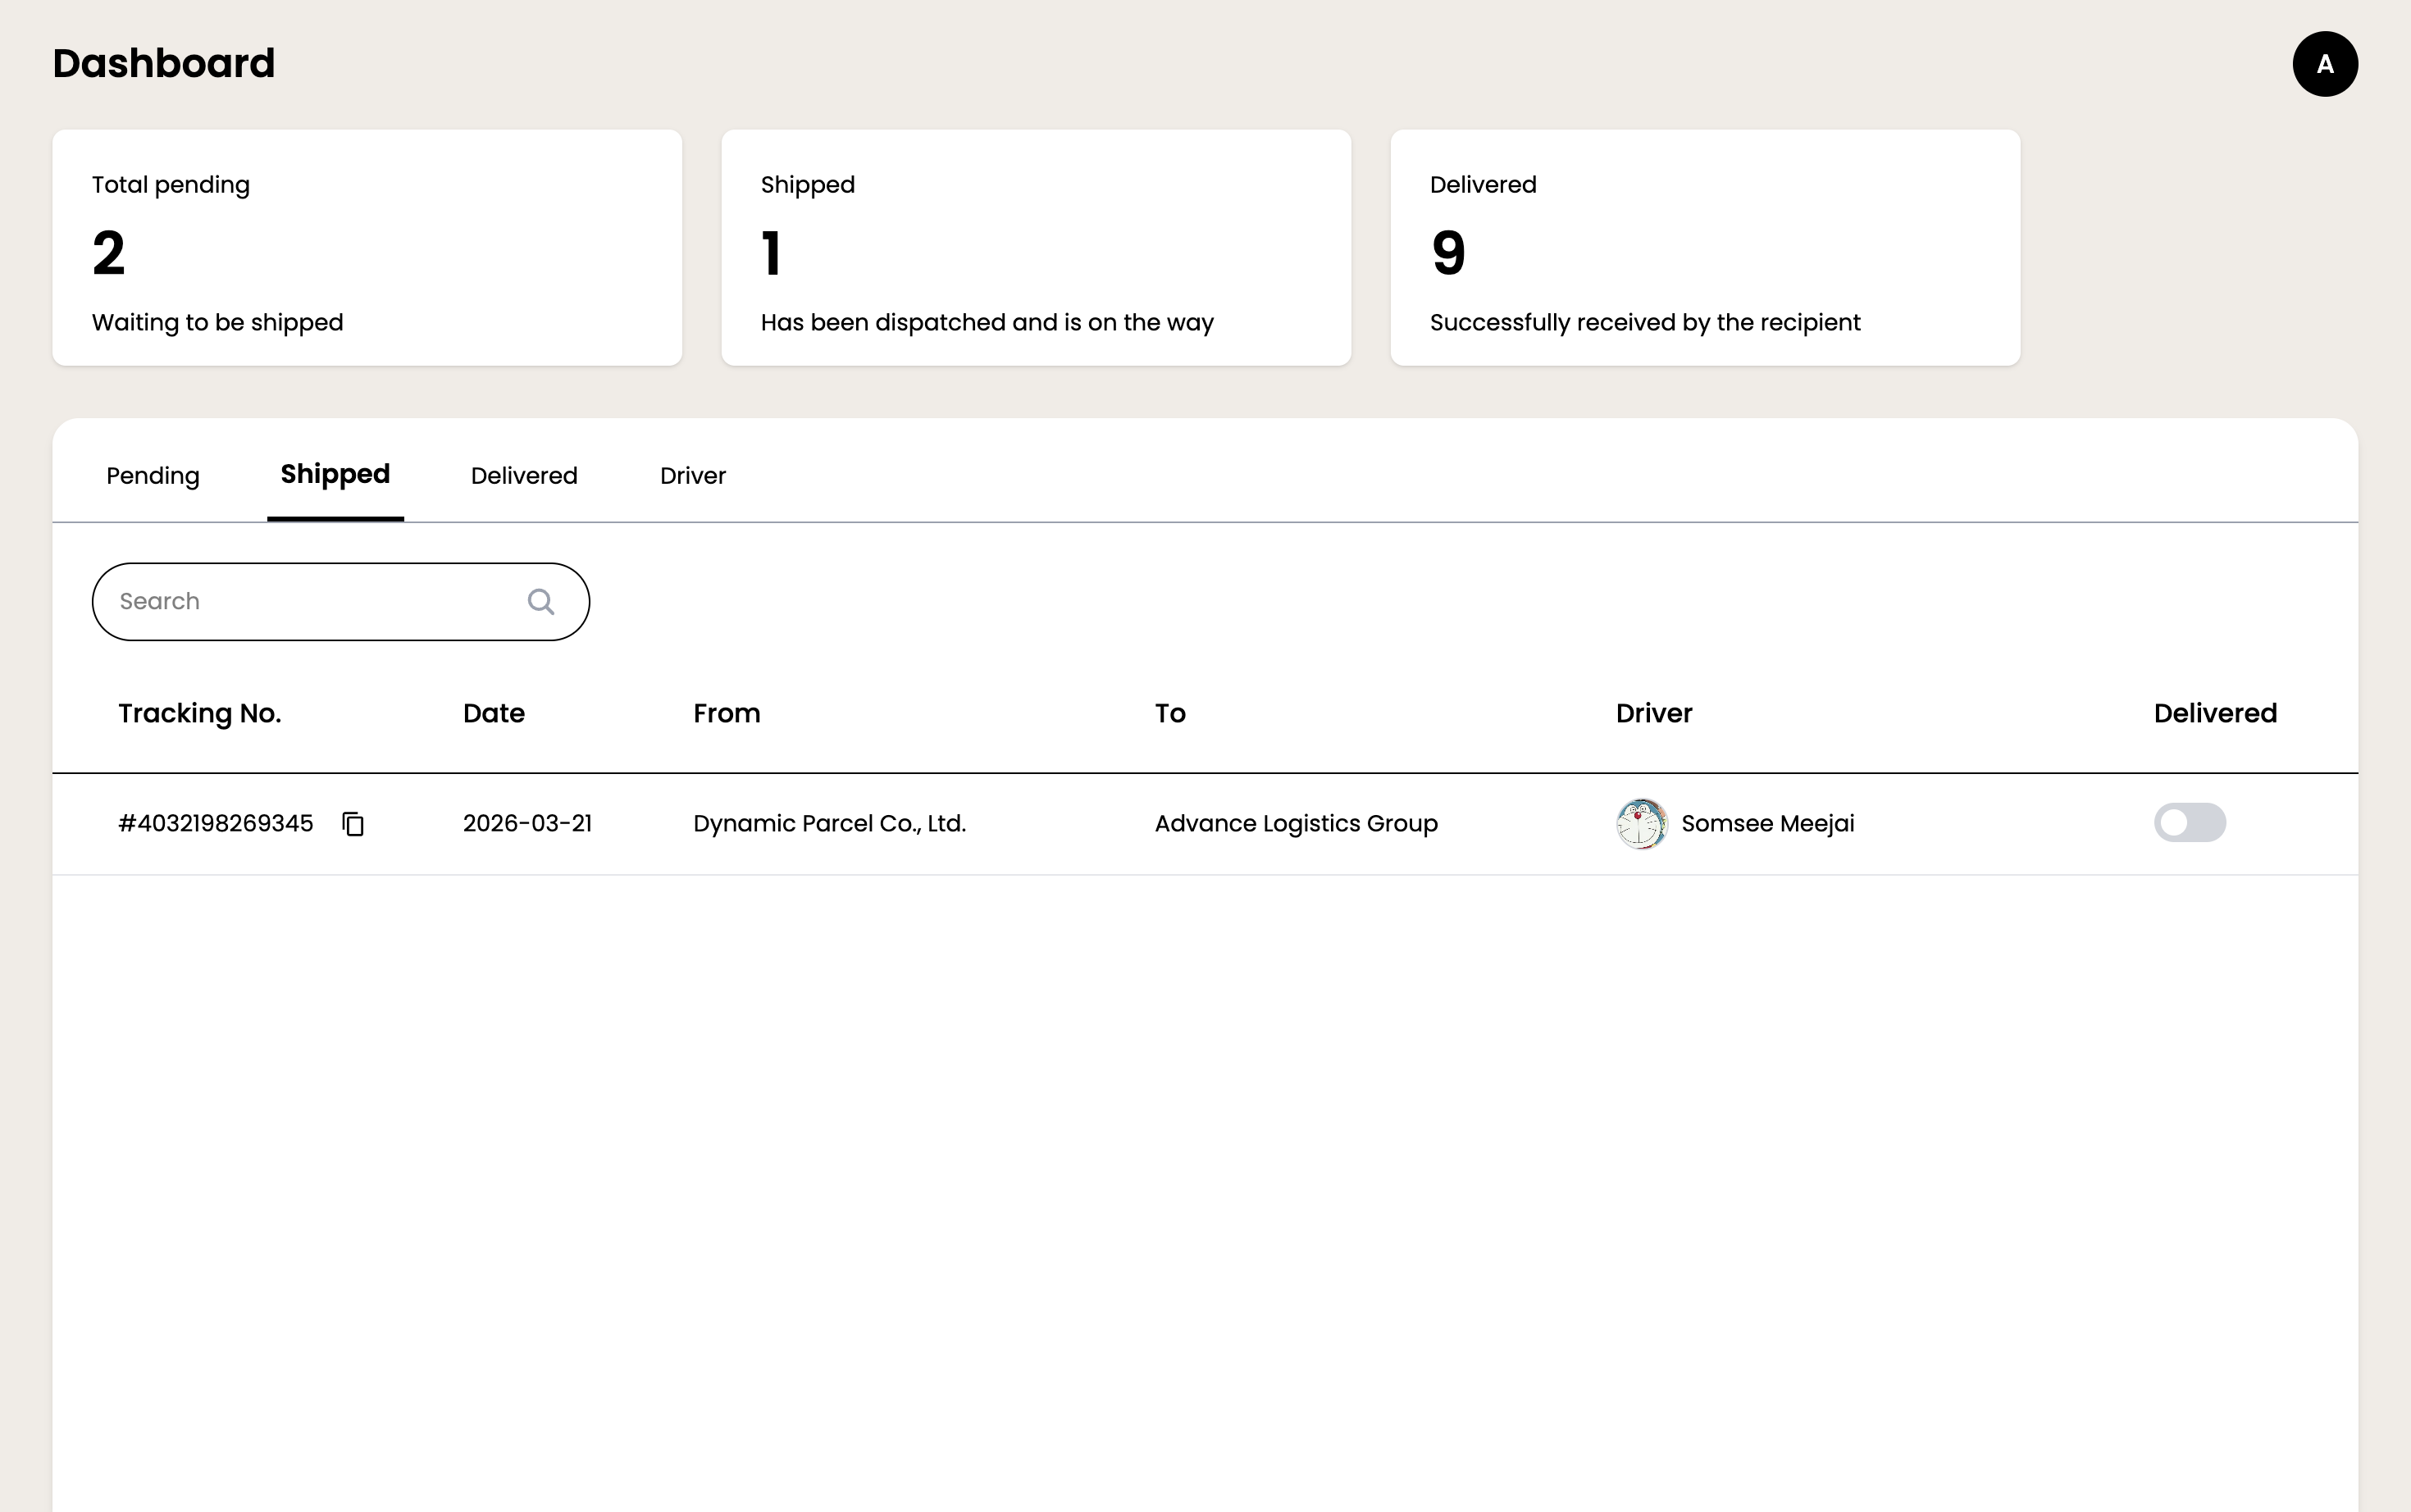
\includegraphics[width=0.8\textwidth]{admin_update_status.png}
    \caption{หน้าเปลี่ยนสถานะพัสดุ}
    \label{fig:ui_admin_update_status}
\end{figure}
\end{minipage}

\vspace{1em}
\begin{minipage}{\linewidth}
\noindent \textbf{5. หน้าประวัติพัสดุที่จัดส่งเสร็จสิ้น} \\
สำหรับดูภาพรวมและตรวจสอบข้อมูลย้อนหลังของพัสดุทั้งหมดที่มีการจัดส่งเสร็จสิ้นสมบูรณ์แล้วในระบบ
\begin{figure}[H]
    \centering
    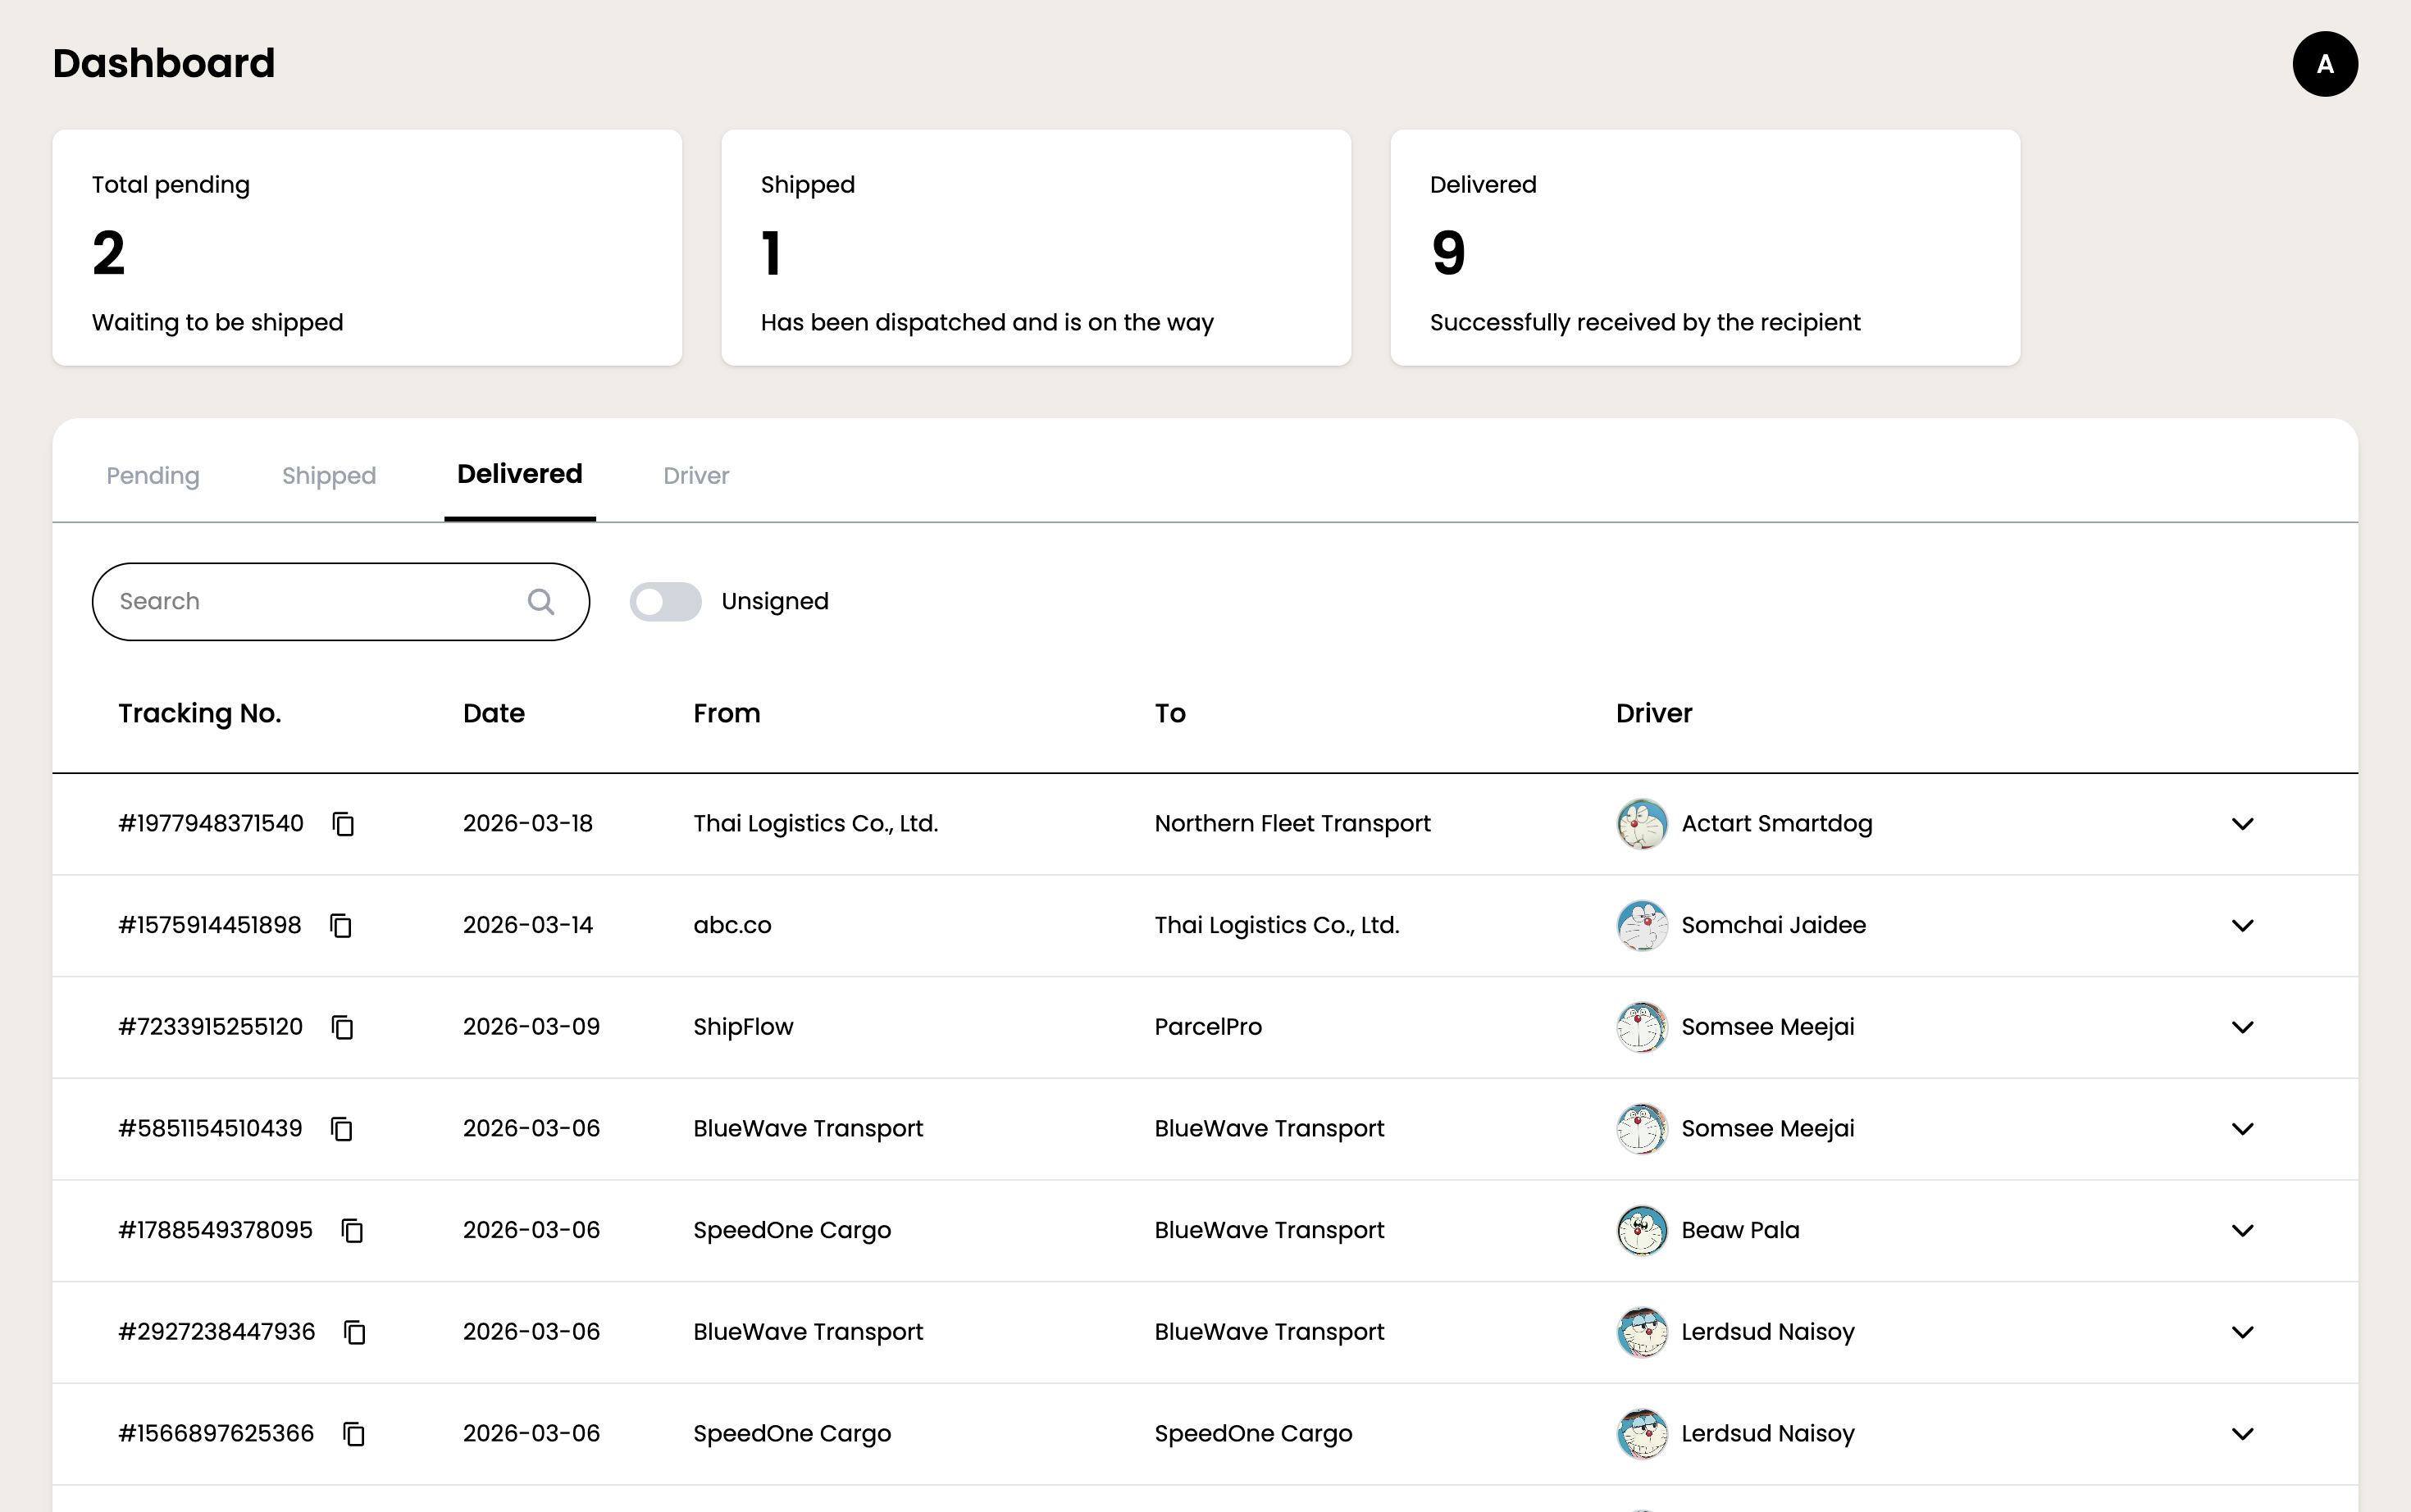
\includegraphics[width=0.8\textwidth]{admin_delivery_history.png}
    \caption{หน้าประวัติพัสดุที่เคยจัดส่งเสร็จแล้วทั้งหมด}
    \label{fig:ui_admin_delivery_history}
\end{figure}
\end{minipage}